\documentclass[11pt]{thesul}

\usepackage{graphicx}
\usepackage[french]{minitoc}
\frenchbsetup{StandardLists=true}
\usepackage{enumitem}
\usepackage[T1]{fontenc}
\usepackage{amsmath}
\usepackage{amsfonts}
\usepackage{amssymb}
\usepackage{graphicx}
\usepackage[counterclockwise]{rotating}
\usepackage{multirow}
\usepackage[usenames, dvipsnames]{xcolor}
\usepackage{tikz}
\usepackage[left=2cm,right=2cm,top=2.5cm,bottom=2.5cm]{geometry}
\usepackage{amsthm}
\usepackage{siunitx}
%\usepackage[ruled]{algorithm}
\usepackage[Algorithme]{algorithm}
\usepackage{algpseudocode}
\alglanguage{pseudocode}

\newtheorem{definition}{D\'efinition}[chapter]
\newtheorem{exemple}{Exemple}[chapter]
\newtheorem{remarque}{Remarque}[chapter]
\newtheorem{proposition}{Proposition}[section]
\newtheorem{theoreme}{Théorème}[chapter]
\newtheorem{lemme}{Lemme}[chapter]
\newtheorem{corollaire}{Corollaire}[chapter]

\def\gint{\displaystyle\int}
\def\gsum{\displaystyle\sum\limits}
\def\gprod{\displaystyle\prod\limits}
\def\longarc{\text{longarc}}
\def\rang{\text{rang}}
\def\REF{\textbf{REF}}
\def\CFL{\text{CFL}}
\def\CS{\text{CS}}
\def\VDM{\text{VDM}}
\def\Id{\text{Id}}
\def\I{\text{I}}
\def\vort{\text{vort}}
\def\rot{\text{rot}}
\def\Sp{\text{Sp}}
\def\Re{\text{Re}}
\def\RK4{\text{RK4}}
\def\dec{\text{déc}}
\def\per{\text{pér}}
\def\vec{\text{vec}}
\def\Vect{\text{Vect}}
\def\arg{\text{arg}}
\def\sech{\text{sech}}
\def\tanh{\text{tanh}}
\def\etafrak{\mathbf{\eta}}
\def\dxi{\tilde{\delta}^H_{\xi}}
\def\deta{\tilde{\delta}^H_{\eta}}
\def\fxi{\tilde{\mathcal{F}}_{\xi}}
\def\feta{\tilde{\mathcal{F}}_{\eta}}
\def\tf{\tilde{f}}
\def\tpz{\text{tpz}}
\def\sps{\text{sps}}
\def\col{\text{col}}

\graphicspath{{./Images/}}

\newcommand\upun[1]{\uppercase{\underline{\underline{#1}}}}
\FormatHeadingsWith\upun

\newcommand\itheadings[1]{\textit{#1}}
\FormatHeadingsWith{\itheadings}

\setlength{\HeadRuleWidth}{0.4pt}

\NoChapterNumberInRef
\NoChapterPrefix

\makeglossary
\makeindex

\begin{document}


      \OddHead={{\leftmark\rightmark}{\hfil\slshape\rightmark}}
      \EvenHead={{\leftmark}{{\slshape\leftmark}\hfil}}
      \OddFoot={\hfil\thepage}
      \EvenFoot={\thepage\hfil}
      \pagestyle{ThesisHeadingsII}

\FrameChaptersInToc  
\ResetChaptersAtParts 
\dominitoc

\ThesisTitle{Schémas compacts hermitiens sur la Sphère - Applications en climatologie et océanographie numérique}
\ThesisDate{3 Juillet 2018}
\ThesisAuthor{Matthieu Brachet}
\ThesisUL

\def\blanc{\hspace*{1cm}}

\President    = {Le président}
\Rapporteurs  = {Eric Blayo\\
                 Thomas Dubos}
\Examinateurs = {Didier Clamond\\
				 Jean-Pierre Croisille\\
				 Michael Ghil\\
				 Véronique Martin\\
                 Dong Ye}

\MakeThesisTitlePage

\begin{ThesisAcknowledgments}
Je remercie le jury, le labo, mon directeur de thèse et tout et tout...
\end{ThesisAcknowledgments}

\begin{ThesisDedication}
Je dédie cette thèse\\
à ma machine.\\
Oui, à Pandore,\\
qui fut la première de toutes.
\end{ThesisDedication}

\WritePartLabelInToc
\WriteChapterLabelInToc

\tableofcontents

%% ************ A COMPLETER PLUS TARD L'INTRO GENERALE
\SpecialSection{Introduction générale}
%% ************ A COMPLETER PLUS TARD L'INTRO GENERALE

%\FrameThisInToc
\DontNumberThisInToc
%\part{Rapport de Thèse}
%\NoChapterHead

\DontWriteThisInToc   
\listoffigures

\WriteThisInToc
\FrameThisInToc
\NumberThisInToc
\part*{Rapport de Thèse}
\mainmatter

%\NumberThisInToc
\chapter{Schémas aux différences}
\label{chap:1}

\section{Opérateurs aux différences en dimension 1}

\subsection{Notations}
\label{sec:notation_1D}

On considère $\Omega = [a,b]$, $a<b$, un intervalle de $\mathbb{R}$ de longueur $L=b-a$. Nous utilisons les lettres latines pour noter les fonctions continues : $f(x)$, $u(x)$, ... $x \in \Omega$ à valeur complexe. Pour $u$ et $v$, des fonctions définies sur $\Omega$, le produit scalaire $L^2 ( \Omega )$ est défini par
\begin{equation}
(u,v) = \gint_{\Omega} u(x) \bar{v}(x) dx = \gint_{a}^b u(x) \bar{v}(x) dx.
\end{equation}
Pour $u$ et $v$ à valeurs réelles, on a
\begin{equation}
(u,v) = \gint_{a}^b u(x) v(x) dx.
\end{equation}
La norme sur $L^2(\Omega)$ est donnée par :
\begin{equation}
\| u \|_{L^2(\Omega)} = \sqrt{(u,u)}.
\end{equation}
Pour $u \in \mathcal
C(\bar{\Omega}) \cap L^{\infty}(\Omega)$, on note
\begin{equation}
\| u \|_{\infty} = \sup_{x\in\Omega} |u(x)|.
\end{equation}
Une fonction $u : x \in \mathbb{R} \mapsto u(x) \in \mathbb{R}$ est \textit{périodique} de période $L$ si 
\begin{equation}
u(x+L) = u(x) \text{, } \forall x \in \mathbb{R}.
\end{equation}
En particulier, on a $u(a)=u(b)$.

On considère une grille régulière sur $\Omega$ constituée de $N + 1$ points :
\begin{equation}
a=x_0 < x_1 < \ldots < x_{N-1} < x_N = b,
\end{equation}
où les valeurs $x_j$ sont définies par :
\begin{equation}
x_j = a + j h\text{, } j = 0,1, \ldots,N \text{ et } h = \dfrac{b-a}{N} \text{ le pas d'espace}. 
\end{equation}

\begin{figure}[htbp]
\begin{center}
\begin{tikzpicture}[scale=1.8]
	\draw [>=stealth, <->] (-2,0.2) -- (-1,.2) ;
	\draw (-1.5,.3) node[above] {$h$} ;
	\draw (-3,0) -- (3,0) ;
	\draw (-3,0) node {$\times$} ;
	\draw (-3,-.2) node[below] {$x_0=a$} ;
	\draw (-2,0) node {$\bullet$} ;
	\draw (-2,-.2) node[below] {$x_1$} ;
	\draw (-1,0) node {$\bullet$} ;
	\draw (-1,-.2) node[below] {$x_2$} ;
	\draw (0,-.2) node[below] {$\ldots$} ;
	\draw (1,0) node {$\bullet$} ;
	\draw (1,-.2) node[below] {$x_{N-2}$} ;
	\draw (2,0) node {$\bullet$} ;
	\draw (2,-.2) node[below] {$x_{N-1}$} ;
	\draw (3,0) node {$\times$} ;
	\draw (3,-.2) node[below] {$x_N =b$} ;
\end{tikzpicture}
\end{center}
\caption{Grille différences finies en dimension 1. Les symboles $\times$ désignent les points de bord, les symboles $\bullet$ désignent les points intérieurs.}
\label{fig:maillage1D}
\end{figure}

Les points $x_0=a$ et $x_N = a + L = b$ sont les points de bord du domaine et les points $(x_j)_{1 \leq j \leq N-1}$ désignent les points intérieurs. 

Nous distinguons trois types de données aux points de grille $x_j$, $0 \leq j \leq N$ :
\begin{enumerate}
\item Une \textit{fonction de grille} est une fonction définie uniquement aux points $(x_j)_{0 \leq j \leq N}$. Les fonctions de grilles sont notées en fonte gothique : $\mathfrak{u}$, $\mathfrak{v}$, ... 
On note
\begin{equation}
\mathfrak{u} = (\mathfrak{u}(x_0), \mathfrak{u}(x_1), \mathfrak{u}(x_2), ... , \mathfrak{u}(x_N)).
\end{equation}
De plus, $l^2_h$ désigne l'espace des fonctions de grille, $h>0$ fixé.
On munit cet espace du produit scalaire $(\cdot, \cdot)_{h}$ et de la norme associée :
\begin{equation}
(\mathfrak{u},\mathfrak{v})_h = h \gsum_{j=0}^N \mathfrak{u}(x_j) \bar{\mathfrak{v}}(x_j) \text{,  } |\mathfrak{u}|_h^2 = h \gsum_{j=0}^N |\mathfrak{u}(x_j)|^2.
\end{equation}
On définit aussi la norme $\| \cdot \|_{\infty}$ pour les fonctions de grille :
\begin{equation}
\| \mathfrak{u} \|_{\infty} = \max_{0\leq j \leq N} |\mathfrak{u}(x_j)|.
\end{equation}
On notera 
\begin{equation}
\mathfrak{u}_j = \mathfrak{u}(x_j) \text{ pour tout } 0\leq j \leq N.  
\end{equation}

On note $l^2_{h,\per}$ l'espace des fonctions de grilles périodiques. Si $\mathfrak{u} \in l^2_{h,\per}$ alors $\mathfrak{u}(x_0) = \mathfrak{u}(x_N)$ et on a
\begin{equation}
\mathfrak{u}=(\mathfrak{u}(x_0), \mathfrak{u}(x_1), ..., \mathfrak{u}(x_{N-1})).
\end{equation}
Le produit scalaire et la norme associée dans $l^2_{h,\per}$ sont
\begin{equation}
(\mathfrak{u},\mathfrak{v})_{h,\per} = h \gsum_{j=0}^{N-1} \mathfrak{u}(x_j) \bar{\mathfrak{v}}(x_j) \text{,  } |\mathfrak{u}|_{h,\per}^2 = h \gsum_{j=0}^{N-1} |\mathfrak{u}(x_j)|^2 \text{ avec } \mathfrak{u}, \mathfrak{v} \in l^2_{h,\per}.
\end{equation}
Pour les fonctions de grille périodiques, on note :
\begin{equation}
\| \mathfrak{u} \|_{\infty} = \max_{0\leq j \leq N-1} |\mathfrak{u}(x_j)|.
\end{equation}



\item Les lettres latines capitales désignent les vecteurs de $\mathbb{R}^{N+1}$ et les matrices de $\mathbb{M}_{N+1}(\mathbb{R})$. Par exemple, le vecteur $U \in \mathbb{R}^{N+1}$ associé à la fonction de grille $\mathfrak{u} \in l^2_h$ est
\begin{equation}
U = \begin{bmatrix}
\mathfrak{u}_0 \\ \mathfrak{u}_1 \\ \vdots \\ \mathfrak{u}_N
\end{bmatrix} =
\begin{bmatrix}
\mathfrak{u}(x_0) \\ \mathfrak{u}(x_1) \\ \vdots \\ \mathfrak{u}(x_N)
\end{bmatrix}.
\end{equation}
La norme euclidienne sur $\mathbb{R}^{N+1}$ est notée $|U|$. Elle induit une norme pour les matrices $A \in \mathbb{M}_{N+1}(\mathbb{R})$ définie par
\begin{equation}
|A|_2 = \sup_{U \neq 0} \dfrac{|AU|}{|U|}.
\end{equation}
Si $A$ est symétrique, l'identité suivante est vérifiée
\begin{equation}
|A|_2 = \rho(A) := \max \left\lbrace |\lambda| \text{ tels que } \lambda \in \Sp (A) \right\rbrace.
\end{equation}
$\rho(A)$ est le \textit{rayon spectrale} de $A$.
De plus, on note également
\begin{equation}
|U|_{\infty} = \max_{1 \leq j \leq N+1} |U_j|.
\end{equation}
La norme sur $\mathbb{M}_{N+1}(\mathbb{R})$ subordonnée à $|\cdot|_{\infty}$ est définie pour $A=(a_{i,j})_{1 \leq i,j \leq N+1} \in \mathbb{M}_{N+1}(\mathbb{R})$ par
\begin{equation}
|A|_{\infty} = \sup_{U \neq 0} \dfrac{|AU|_{\infty}}{|U|_{\infty}} = \max_{1 \leq i \leq N+1} \gsum_{j=1}^{N+1} |a_{i,j}|.
\end{equation}



\item Soit $u: x \in \Omega \mapsto u(x)$, on définit la \textit{fonction de grille} $u^*$ associée à $u$ par :
\begin{equation}
u^*_j = u^*(x_j) \text{ pour } 0 \leq j \leq N,
\end{equation}
$u^*$ est donc la restriction de $u$ aux points de la grille. Si $u$ est une fonction $L-$périodique, alors $u^*$ est définie par
\begin{equation}
u^*_j = u^*(x_j) \text{ pour } 0 \leq j \leq N-1.
\end{equation}
\end{enumerate}

Nous distinguons $l^2_h$, l'espace des fonctions de grilles d'une part, et d'autres part l'espace vectoriel $\mathbb{R}^{N+1}$ même si ces deux espaces sont isomorphes.

Cette distinction permet de faire une claire différence entre :
\begin{itemize}
\item les opérateurs aux différences finies, qui agissent sur les fonctions de grille,
\item les matrices, qui agissent sur les vecteurs.
\end{itemize}
Les fonctions de grilles contiennent toutes les échelles nécessaires dans le contexte physique alors que les vecteurs sont sans dimension. De plus, le raisonnement au niveau discret est plus naturel avec les fonctions de grilles. Il s'effectue d'une façon abstraite à l'aide d'opérateurs aux différences. En revanche, le codage est effectué dans le cadre de l'espace vectoriel $\mathbb{R}^{N+1}$.

On note que trois normes infinies ont été définies :
\begin{itemize}
\item l'écriture $\| \cdot \|_{\infty}$ désigne à la fois la norme pour une fonction $u$ définie sur $\Omega$ ou une fonction de grille $\mathfrak{u}$. Le contexte permettra de distinguer les deux cas de figure.
\item La notation $| \cdot |_{\infty}$ désigne la norme d'une matrice $A$ ou d'un vecteur $U$. La distinction se fera en fonction du contexte.
\end{itemize}




















\subsection{Transformée de Fourier discrète}

Quitte à opérer une translation sur $x$, on peut supposer $a=0$ et $b=L$. Le pas du maillage est $h = \frac{L}{N}$.
Soit, pour tout $k$ vérifiant $-N/2+1 \leq k \leq N/2$, la fonction $u^k : x \mapsto u^k(x) \in \mathbb{C}$ périodique de période $L$ définie par 
\begin{equation}
u^k(x) = \dfrac{1}{\sqrt{L}} \exp \left( \dfrac{2 i \pi k x}{L} \right).
\end{equation}
Les fonctions $(u^k)_{-N/2 +1 \leq k \leq N/2}$ forment une famille libre et orthonormée de $N+1$ fonctions. C'est à dire
\begin{equation}
(u^k, u^{k'})_{L^2([a,b])} = \delta_{k,k'} \text{ avec } -N/2+1 \leq k, k' \leq N/2.
\end{equation}
On définit les \textit{fonctions de base} $\mathfrak{u}^k$ de $l^2_{h,\per}$ par
\begin{equation}
\mathfrak{u}^k = \sqrt{h} (u^k)^*
\end{equation}
donc 
\begin{equation}
\mathfrak{u}^k_j = \sqrt{h}  u^k(x_j) = \dfrac{1}{\sqrt{N}} \exp \left( \dfrac{2 i \pi j k h}{L} \right) = \dfrac{1}{\sqrt{N}} \exp \left( \dfrac{2 i \pi j k}{N} \right) \text{ avec } 0 \leq j \leq N-1.
\label{eq:base_fourier_disc}
\end{equation}


\begin{proposition}
Les fonctions $(\mathfrak{u}^k)_{-N/2+1 \leq k \leq N/2}$ forment une base orthonormée de $l^2_{h,\per}$.
\end{proposition}

\begin{proof}
On montre que $(\mathfrak{u}^k)_{-N/2+1 \leq k \leq N/2}$ satisfait
\begin{equation}
(\mathfrak{u}^k, \mathfrak{u}^{k'})_{h,\per} = \delta_{k,k'}
\end{equation}
pour tous $-N/2+1 \leq k, k' \leq N/2$.

Considérons d'abord $k$ et $k'$ sont deux entiers distincts tels que $-N/2+1 \leq k, k' \leq N/2$. $\mathfrak{u}^k, \mathfrak{u}^{k'} \in l^2_{h,\per}$ et
\begin{align*}
(\mathfrak{u}^k, \mathfrak{u}^{k'})_{h,\per} & = \dfrac{1}{N} \gsum_{j=0}^{N-1} \exp \left( \dfrac{2 i \pi j k}{N} \right) \exp \left( -\dfrac{2 i \pi j k'}{N} \right) \\
		& = \dfrac{1}{N} \gsum_{j=0}^{N-1} \exp \left( i j (k-k') \dfrac{2 \pi}{N} \right)\\
		& = \dfrac{1}{N} \dfrac{1 - \exp \left( i 2 \pi (k-k') \right)}{1 - \exp \left( i (k-k') \dfrac{2 \pi}{N}  \right)} \\
		& = 0.
\end{align*}
De plus, si $k=k'$, on a :
\begin{align*}
(\mathfrak{u}^k, \mathfrak{u}^{k'})_{h,\per} & = \dfrac{1}{N} \gsum_{j=0}^{N-1} \exp \left( \dfrac{2 i \pi j k}{N} \right) \exp \left( -\dfrac{2 i \pi j k'}{N} \right) \\
		& = \dfrac{1}{N} \gsum_{j=0}^{N-1} 1 \\
		& = 1.
\end{align*}
D'où le résultat.
\end{proof}

Pour tout $\mathfrak{v} \in l^2_{h,\per}$, on note $(\hat{\mathfrak{v}}_k )_{-N/2 \leq k \leq N/2}$ les composants de $\mathfrak{v}$ sur la base $(\mathfrak{u}^k)_{-N/2 +1 \leq k \leq N/2}$ :
\begin{equation}
\mathfrak{v} = \gsum_{-N/2+1}^{N/2} \hat{\mathfrak{v}}_k \mathfrak{u}^k.
\end{equation}
En effectuant le produit scalaire par $\mathfrak{u}^{k'}$ on obtient
\begin{align*}
(\mathfrak{v}, \mathfrak{u}^{k'})_{h,\per} & = \gsum_{k=-N/2+1}^{N/2} \hat{\mathfrak{v}}^k \underbrace{(\mathfrak{u}^k, \mathfrak{u}^{k'})_{h,\per}}_{\delta_{k,k'}} \\
		& = \hat{\mathfrak{v}}_{k'}
\end{align*}

\begin{definition}
On définit la \textit{transformée de Fourier discrète} de $\mathfrak{v}$ par $(\hat{\mathfrak{v}}_{k})_{-N/2+1 \leq k \leq N/2}$ où
\begin{equation}
\hat{\mathfrak{v}}_{k} = (\mathfrak{v}, \mathfrak{u}^{k})_{h,\per}.
\end{equation}
\end{definition}

\begin{proposition}
\textbf{(Relation de Parseval discrète)} 
Pour tout $\mathfrak{v} \in l^2_{h,\per}$, on a 
\begin{equation}
|\mathfrak{v}|_{h,\per}^2 = \gsum_{k=-N/2+1}^{N/2} |\hat{\mathfrak{v}}_k|^2
\end{equation}
\end{proposition}

\begin{proof}
On sait que 
\begin{equation}
|\mathfrak{v}|_{h,\per}^2 = \gsum_{j=0}^{N-1} \mathfrak{v}_j \bar{\mathfrak{v}}_j.
\end{equation}
Or par décomposition, on a
\begin{equation}
\begin{array}{rcl}
\mathfrak{v}_j & = & \gsum_{k = -N/2+1}^{N/2} \hat{v}_k \mathfrak{u}_j^k \\
\bar{\mathfrak{v}}_j & = & \gsum_{k' = -N/2+1}^{N/2} \bar{\hat{\mathfrak{v}}}_{k'} \bar{\mathfrak{u}}_j^{k'}.
\end{array}
\end{equation}
Alors, on obtient
\begin{align*}
|\mathfrak{v}|_{h,\per}^2 & = h \gsum_{j=0}^{N-1} \gsum_{k=-N/2+1}^{N/2} \gsum_{k'=-N/2+1}^{N/2} \hat{\mathfrak{v}}_j \mathfrak{u}_j^k \bar{\hat{\mathfrak{v}}}_j \bar{\mathfrak{u}}_j^{k'} \\
	& = h \gsum_{k=-N/2+1}^{N/2} \gsum_{k'=-N/2+1}^{N/2} \hat{\mathfrak{v}}_k \bar{\hat{\mathfrak{v}}}_{k'} \gsum_{j=0}^{N-1} \mathfrak{u}_j^k \bar{\mathfrak{u}}_j^{k'} \\
	& = \gsum_{k=-N/2+1}^{N/2} \gsum_{k'=-N/2+1}^{N/2} \hat{\mathfrak{v}}_k \bar{\hat{\mathfrak{v}}}_{k'} (\mathfrak{u}^k, \mathfrak{u}^{k'})_{h,\per}.
\end{align*}
Or on sait que $(\mathfrak{u}^k, \mathfrak{u}^{k'})_{h,\per} = \delta_{k,k'}$ donc
\begin{align*}
|\mathfrak{v}|_{h,\per}^2 & = \gsum_{k=-N/2+1}^{N/2} \gsum_{k'=-N/2+1}^{N/2} \hat{\mathfrak{v}}_k \bar{\hat{\mathfrak{v}}}_{k'} \delta_{k,k'}\\
	& = \gsum_{k=-N/2+1}^{N/2} \hat{\mathfrak{v}}_k \bar{\hat{\mathfrak{v}}}_k \\
	& = \gsum_{k=-N/2+1}^{N/2} |\hat{\mathfrak{v}}_k|^2.
\end{align*}
Ce qui conclut la démonstration.
\end{proof}

















\subsection{Opérateur de translation périodique}
On se donne $\mathfrak{u} \in l^2_{h,\per}$ une fonction de grille périodique.
\begin{definition}
L'opérateur $\tau_p$, $p \in \mathbb{Z}$, est défini, pour $\mathfrak{u}$ fonction de grille périodique, par
\begin{equation}
(\tau_p \mathfrak{u})_j = \mathfrak{u}_{j+p} \text{ avec } 0 \leq j \leq N-1.
\end{equation}
\end{definition}
L'opérateur linéaire $\tau_p$ agit sur les fonctions périodiques $u : \mathbb{R} \mapsto u(x) \in \mathbb{R}$ par :
\begin{equation}
(\tau_p u)^*_j = \tau_p u(x_j) = u(x_{j+p}) = u^*_{j+p}.
\end{equation}
En particulier, lorsque $p=1$, on note $\tau$ l'\textit{opérateur de translation à droite} :
\begin{equation}
\tau = \tau_{1}.
\end{equation}
De plus, il est clair que l'on a
\begin{equation}
\begin{array}{rcl}
\text{i)   }\tau^0 & = & \Id\\
\text{ii)  }\tau^p & = & \underbrace{\tau \circ \tau \circ \tau \circ \cdots \circ \tau}_{p \text{ fois.}} = \tau_p.
\end{array}
\end{equation}
En particulier, $\tau^N = \tau_N = \Id$, donc $\tau$ est inversible et
\begin{equation}
\tau^{-1} = \tau^{N-1}.
\end{equation}
L'analyse des opérateurs périodiques repose sur la diagonalisation de $\tau$. C'est l'objet de la proposition suivante. On note
\begin{equation}
\omega = \exp \left[ \dfrac{2 i \pi}{N} \right]
\end{equation}
ainsi que
\begin{equation}
\omega^k = \exp \left[ \dfrac{2 i k \pi}{N} \right]
\end{equation}
pour $-N/+1 \leq k \leq N/2$, les racines $N-$ièmes de l'unité.
\begin{proposition}
\begin{itemize}
\item Les valeurs propres de $\tau$ sont $\omega^k \in \mathbb{C}$, $-N/2 + 1 \leq k \leq N/2$,

\item L'espace propre associé à $\omega^k$ est $\Vect (\mathfrak{u}^k)$. En particulier, $\tau$ est diagonalisable et sa décomposition spectrale est
\begin{equation}
\tau = \gsum_{k = -N/2+1}^{N/2} \omega^k p_k
\end{equation}
où $p_k$ est le projecteur orthogonale sur $\Vect (\mathfrak{u}^k)$, pour tout $\mathfrak{v} \in l^2_{h,\per}$ et $-N/2+1 \leq k \leq N/2$
\begin{equation}
p_k \mathfrak{v} = (\mathfrak{v},\mathfrak{u}^k)_{h,\per}\mathfrak{u}^k.
\label{eq:projecteurspectrale}
\end{equation}
\end{itemize}
\label{prop:eigenvaluevector_tau}
\end{proposition}

\begin{proof}
Soient $j, k$ tels que $0 \leq j \leq N-1$ et $-\frac{N}{2}+1 \leq k \leq \frac{N}{2}$. On a
\begin{equation}
(\tau \mathfrak{u}^k)_j = \mathfrak{u}^k_{j+1}= \dfrac{1}{\sqrt{N}}\exp \left[ \dfrac{2 i (j+1)  \pi k}{N} \right] = \dfrac{1}{\sqrt{N}} \exp \left[ \dfrac{2 i j \pi k}{N} \right] \exp \left[ \dfrac{2 i \pi k}{N} \right] = \omega^k \mathfrak{u}_j^k.
\end{equation}
L'opérateur $\tau$ possède $N$ valeurs propres distinctes, il est diagonalisable et sa décomposition spectrale s'obtient par la formule
\begin{equation*}
\tau = \gsum_{k = -N/2+1}^{N/2} \omega^k p_k.
\end{equation*}
\end{proof}

Soit $P \in \mathbb{C}[X]$ un polynôme. Les valeurs propres et les fonctions propres de $P(\tau)$ sont données par la proposition suivante:
\begin{proposition}
\begin{itemize}
\item Les valeurs propres de $P(\tau)$ sont $P(\omega^k) \in \mathbb{C}$, $-N/2 + 1 \leq k \leq N/2$,

\item L'espace propre associé à $P(\omega^k)$ est $\Vect (\mathfrak{u}^k)$. $P(\tau)$ est diagonalisable, sa décomposition spectrale est
\begin{equation}
P(\tau) = \gsum_{k=-N/2+1}^{N/2} P(\omega^k) p_k
\label{eq:formule_diagPtau}
\end{equation}
où $p_k$ est le projecteur donné par \eqref{eq:projecteurspectrale}.
\end{itemize}
\label{prop:eigen_Ptau}
\end{proposition}

\begin{proof}
$P$ est un polynôme de $\mathbb{C}[X]$ donc il existe un nombre fini d'éléments de $\mathbb{C}$ notés $a_0$, $a_1$, $a_2$, ... tels que
\begin{equation}
P(X) = \gsum_{n} a_n X^n.
\end{equation}
Soient $j, k$ tels que $0 \leq j \leq N-1$ et $-\frac{N}{2}+1 \leq k \leq \frac{N}{2}$. On a
\begin{align*}
(P(\tau)\mathfrak{u}^k)_j = & \left( \gsum_{n} a_n \tau^n \mathfrak{u}^k  \right)_j\\
	& = \gsum_n a_n \mathfrak{u}^k_{j+n}.
	\end{align*}
Or par construction de $\mathfrak{u}^k$, on a
\begin{align*}	
(P(\tau)\mathfrak{u}^k)_j & = \gsum_{n} a_n (\omega^k)^n \mathfrak{u}_j^k \\
	& = P(\omega^k) \mathfrak{u}_j^k,
\end{align*}
donc $P(\omega^k)$ est valeur propre de $P(\tau)$.
De plus, les espaces vectoriels $\Vect (\mathfrak{u}^k)$ sont en somme directe, donc $P(\tau)$ est diagonalisable et la formule  est \eqref{eq:formule_diagPtau} vérifiée.
\end{proof}

\begin{remarque}
Noter que cette proposition est vraie non seulement pour $\tau$ mais aussi pour tout opérateur diagonalisable.
\end{remarque}

On définit $\vec_1$ l'opérateur appliquant un élément de $l_{h,\per}^2$ sur un vecteur de $\mathbb{R}^N$ :

\begin{definition}
Soient $\mathfrak{u} \in l^2_{h,\per}$ une fonction de grille et $(\mathbf{e}_j)_{1 \leq j \leq N}$ la base canonique de $\mathbb{R}^N$. On définit l'opérateur $\vec_1$ par :
\begin{equation}
\begin{array}{rcl}
\vec_1 : l^2_{h,\per} & \rightarrow & \mathbb{R}^N \\
         \mathfrak{u} & \mapsto & \vec_1 ( \mathfrak{u} )
\end{array}
\end{equation}
avec 
\begin{equation}
\vec_1 (\mathfrak{u} ) = \gsum_{j=1}^N \mathfrak{u}_{j-1} \mathbf{e}_j
\end{equation}
\end{definition}
Lorsque cela ne porte à aucune confusion, nous noterons $\vec$ au lieu de $\vec_1$. La distinction se fera aisément en fonction du contexte.

Pour toute fonction de grille $\mathfrak{u} \in l^2_{h,\per}$ on note
\begin{equation}
U = \vec( \mathfrak{u} ) = \vec_1( \mathfrak{u} ) = \begin{bmatrix}
\mathfrak{u}_0\\
\mathfrak{u}_1\\
\vdots\\
\mathfrak{u}_{N-1}\\
\end{bmatrix} \in \mathbb{R}^N
\end{equation}

On s'intéresse à présent à l'interprétation matricielle de $\tau$. On note $T \in \mathbb{M}_N (\mathbb{R})$ la matrice donnée par
\begin{equation}
T = \begin{bmatrix}
0 & 1 &   &   &   \\ 
  & 0 & 1 & (0) &   \\ 
  &   & \ddots & \ddots &   \\ 
  & (0) &   & 0 & 1 \\ 
1 &   &   &   & 0
\end{bmatrix} 
\label{eq:matrice_translation}
\end{equation}

La matrice $T$ agit sur un vecteur $U = \begin{bmatrix}
U_1 & U_2 & \cdots & U_{N} 
\end{bmatrix}^T \in \mathbb{R}^N $ par
\begin{equation}
(TU)_j = U_{j+1} \text{ avec } 1 \leq j \leq N.
\end{equation}
C'est à dire
\begin{equation}
\vec ( \tau \mathfrak{u} ) = T ( \vec ( \mathfrak{u} ) ). 
\end{equation}
Les propriétés spectrales de $T$ se déduisent de celles de $\tau$ :
\begin{corollaire}
\label{cor:eigen_P(T)}
\begin{itemize}
\item Les valeurs propres de $T$ sont les valeurs $(\omega^k)_{-N/2+1 \leq k \leq N/2}$. 
L'espace vectoriel associé est $\Vect ( U^k )$ avec
\begin{equation}
U^k = \vec (\mathfrak{u}^k ).
\label{eq:eigenvectorT}
\end{equation}
$\mathfrak{u}^k$ et $\omega$ sont donnés par la proposition \ref{prop:eigenvaluevector_tau}.

\item Si $P \in \mathbb{R}[X]$ alors les valeurs propres de $P(T)$ sont $P(\omega^k)$ avec $-N/2 + 1 \leq k \leq N/2$ et l'espace propre associé est \eqref{eq:eigenvectorT}.
\end{itemize}
\end{corollaire}

Les vecteurs $(U^k)_{-N/2+1 \leq k \leq N/2}$ forment une base orthonormée de $\mathbb{R}^N$ pour le produit scalaire usuel.



















\subsection{Opérateurs aux différences discrets}

Dans cette section on s'intéresse à une approximation symétrique de $\partial_x : u \in \mathcal{C}^1 \mapsto \partial_x u \in \mathcal{C}^0$ de la forme
\begin{equation}
\delta_{2J,x} = \gsum_{p=1}^J a_p \dfrac{\tau_p - \tau_{-p}}{2 p h}
\label{eq:explicite_dx}
\end{equation}
C'est le type d'opérateur dont nous aurons besoin dans la suite pour la calcul approché d'opérateurs sphériques.

Cette question est classique en analyse numérique. Elle est abordée dans des références classiques telles que \cite{Ames2014, Collatz2012, Kopal1955}. En mathématiques, on cite en particulier \cite{Collatz2012, Kopal1955} ou en mécanique des fluides numériques \cite{Hirsch2007}.

Nous commençons par rappeler la \textit{consistance} d'un opérateur différentiel \cite{Strikwerda2004}. On s’intéresse à l'équation aux dérivées partielles
\begin{equation}
\mathcal{L}u = f
\end{equation}
où $f$ est une fonction donnée. L'équation est discrétisée en
\begin{equation}
L_h \mathbf{u} = f^* .
\end{equation}
La consistance est définie par
\begin{definition}
le couple $(L_h, R_h)$ est consistant avec $\mathcal{L}$ à l'ordre $\alpha$ si pour toute fonction $u$ régulière, on a
\begin{equation}
L_h (u^*) -R_h \left( \mathcal{L}u \right) = \mathcal{O}(h^{\alpha})
\end{equation}
avec $R_h$ un opérateur d'interpolation approchant l'identité. $L_h (u^*) -R_h \left( \mathcal{L}u \right)$ est \textit{l'erreur de troncature}.
\label{def:consistance}
\end{definition}


\begin{itemize}
\item \textbf{Exemple 1 : }L'opérateur aux différences centré usuel est
\begin{equation}
\delta_x = \dfrac{\tau_1 - \tau_{-1}}{2h}.
\label{eq:deltax2}
\end{equation}
Appliqué à la fonction de grille $\mathfrak{u}$, cet opérateur s'exprime par 
\begin{equation}
\delta_x \mathfrak{u}_j = \dfrac{\mathfrak{u}_{j+1} - \mathfrak{u}_{j-1}}{2h} \text{ pour } 0 \leq j \leq N-1.
\end{equation}
Il s'agit d'un opérateur qui approche la dérivée première. On a :
\begin{proposition}
Soit $u: x \in \Omega \mapsto u(x) \in \mathbb{R}$ et $u^*$ la fonction de grille correspondante. Si $u \in \mathcal{C}^3 (\Omega)$ alors 
\begin{equation}
\delta_x u^*_j - \partial_x u(x_j) = \dfrac{h^2}{6} \partial_x^{(3)}u(\alpha) \text{ avec } \alpha \in ]x_{j-1}, x_{j+1}[,
\end{equation}
\label{prop:eq_deltax2}
\end{proposition}

\begin{proof}
Pour $u$ de classe $\mathcal{C}^3$, on considère les développements de Taylor-Lagrange :
\begin{equation}
u(x_j+h) = u(x_j) + h \partial_x u(x_j) + \dfrac{h^2}{2} \partial_x^{(2)} u(x_j) + \dfrac{h^3}{6} \partial_x^{(3)}u (\eta) \text{ avec } \eta \in ]x_j, x_{j+1}[
\end{equation}
et également :
\begin{equation}
u(x_j-h) = u(x_j) - h \partial_x u(x_j) + \dfrac{h^2}{2} \partial_x^{(2)} u(x_j) - \dfrac{h^3}{6} \partial_x^{(3)} u(\xi) \text{ avec } \xi \in ]x_{j-1}, x_{j}[.
\end{equation}
Alors par différence, on obtiens : 
\begin{equation}
\delta_x u^*_j = \partial_x u(x_j) + \dfrac{h^2}{12} \left[ \partial_x^{(3)} u(\xi) + \partial_x^{(3)} u (\eta) \right]  \text{ avec } \xi, \eta \in ]x_{j-1}, x_{j+1}[.
\end{equation}
Comme $u$ est de classe $\mathcal{C}^{3}$, $\partial_x^{(3)}u$ est continue. Donc il existe $\alpha \in ]\xi, \eta[ \subset ]x_{j-1}, x_{j+1}[$ tel que
\begin{equation}
2 \partial_x^{(3)}u(\alpha) = \partial_x^{(3)} u(\xi) + \partial_x^{(3)} u (\eta)
\end{equation}
d'où on obtient 
\begin{equation}
\delta_x u^*_j - \partial_x u(x_j) = \dfrac{h^2}{6} \partial_x^{(3)}u(\alpha) \text{ avec } \alpha \in ]x_{j-1}, x_{j+1}[.
\end{equation}
\end{proof}
Il résulte de la proposition \ref{prop:eq_deltax2} que \eqref{eq:deltax2} est consistant à l'ordre 2 au sens de la définition \ref{def:consistance} avec $R_h = \Id$.



\item \textbf{Exemple 2 :} Une manière d'augmenter la consistance de l'exemple 1 est de modifier l'opérateur $R_h$ \cite{Collatz2012}. Pour cela on introduit $\sigma_x$ l'opérateur de Simpson
\begin{equation}
\sigma_x = \dfrac{1}{6} \tau + \dfrac{4}{6} \Id + \dfrac{1}{6} \tau^{-1}.
\end{equation}
Si $\mathfrak{u} \in l^2_{h,\per}$ est une fonction de grille alors
\begin{equation}
\sigma_x \mathfrak{u}_j = \dfrac{1}{6} \mathfrak{u}_{j+1} + \dfrac{4}{6} \mathfrak{u}_j + \dfrac{1}{6} \mathfrak{u}_{j-1} .
\end{equation}
La proposition suivante est alors vérifiée :
\begin{proposition}
Soit $u : x \in \Omega \mapsto u(x) \in \mathbb{R}$ et $u^*$ la fonction de grille associée. Si $u \in \mathcal{C}^5(\Omega)$ alors 
\begin{equation}
\| \sigma_x \partial_x u^*_j - \delta_x u^*_j \|_{\infty} \leq \dfrac{h^4}{45} \| \partial_x^{(5)} u \|_{\infty}.
\end{equation}
\label{prop:eq_deltax2_sigmax}
\end{proposition}

\begin{proof}
Soit $f$ une fonction régulière de $\Omega$ dans $\mathbb{R}$. Pour $0 \leq j \leq N-1$, on pose
\begin{equation}
\mathfrak{e}_j = \dfrac{h}{3} \left[ f(x_{j-1}) + 4 f(x_j) + f(x_{j+1}) \right] - \gint_{x_{j-1}}^{x_{j-1}} f(x) dx = 2h \sigma_x f^*_j - \gint_{x_{j-1}}^{x_{j-1}} f(x) dx.
\end{equation}
Il s'agit de l'erreur de quadrature de la formule de Simpson.
D'une part, par développement de Taylor, on a
\begin{equation}
2h \sigma_x f^*_j = 2h f(x_j) + \dfrac{h}{3}\partial_x^{(2)}f(x_j) + \dfrac{h^5}{72} \left( \partial_x^{(4)}f(\xi) + \partial_x^{(4)}f(\eta) \right) 
\end{equation}
avec $\xi \in ]x_{j-1}, x_j[$ et $\eta \in ]x_j, x_{j+1}[$.
D'autres part, au voisinage $]x_{j-1}, x_{j+1}[$ de $x_j$ et en posant $t=x-x_j$, on a 
\begin{equation}
f(x) = f(x_j) + t \partial_x f(x_j) + \dfrac{t^2}{2} \partial_x^{(2)} f(x_j) + \dfrac{t^3}{6} \partial_x^{(3)} f(x_j) + \dfrac{t^4}{24} \partial_x^{(4)} f(\omega)
\end{equation}
avec $\omega \in ]x_{j-1}, x_{j+1}[$. On intègre cette dernière équation d'où
\begin{align*}
\gint_{x_{i-1}}^{x_{i+1}} f(x) dx & = \gint_{-h}^h \left( f(x_j) + t \partial_x f(x_j) + \dfrac{t^2}{2} \partial_x^{(2)} f(x_j) + \dfrac{t^3}{6} \partial_x^{(3)} f(x_j) + \dfrac{t^4}{24} \partial_x^{(4)} f(\omega) \right) dt \\
	& = 2h f(x_j) + \dfrac{h}{3}\partial_x^{(2)}f(x_j) + \dfrac{h^5}{60}\partial_x^{(4)} f(\omega).
\end{align*}
Alors, par comparaison, on trouve
\begin{align*}
|\mathfrak{e}_j| & = |\dfrac{h^5}{72} \left( \partial_x^{(4)}f(\xi) + \partial_x^{(4)}f(\eta) \right)  - \dfrac{h^5}{60}\partial_x^{(4)} f(\omega)|  \\
	& \leq \dfrac{2 h^5}{45} \max_{x} |\partial_x^{(4)} f(x)|.
\end{align*}
Pour conclure, on applique la formule précédente avec $f = \partial_x u$. On note que 
\begin{equation}
\gint_{x_{i-1}}^{x_{i+1}}f(x) dx = u(x_{i+1}) - u(x_{i-1}),
\end{equation}
de là, on obtient
\begin{equation}
|\sigma \left( \partial_x u^* \right)_j - \delta_x u^*_j | \leq \dfrac{h^5}{45}\max_{x} |\partial_x^{(4)} f(x)|
\end{equation}
et on peut conclure directement.
\end{proof}
De la proposition \ref{prop:eq_deltax2_sigmax}, il découle que le couple $(L_h, R_h) = (\delta_x, \sigma_x)$ est consistant avec la dérivée première à l'ordre $4$.
\end{itemize}

On s'intéresse à présent aux opérateurs centré et antisymétriques dont le stencil est composé de $2J+1$ points de la forme \eqref{eq:explicite_dx}. L'intérêt de cette famille d'opérateur réside en l'absence de dissipation numérique. On choisi dans ce travail de maximiser l'ordre de consistance de ces opérateurs mais d'autres options sont possibles. On citera en particulier les schémas peu dispersifs \cite{Bogey2004} ou les schémas du type "dispersion relation preserving" \cite{Tam1993}.

\begin{theoreme}
Soit $f : \Omega \rightarrow \mathbb{R}$ alors l'identité discrète
\begin{equation}
\delta_{2J,x} \mathfrak{u} = f^*
\end{equation}
est consistante à l'ordre $2J$ avec 
\begin{equation}
\partial_x u = f
\end{equation}
(avec $R_h = \Id$ et $L_h = \delta_{2J,x}$) si et seulement si les coefficients $(a_p)_{1 \leq p \leq J}$ sont solution du système
\begin{equation}
\left\lbrace
\begin{array}{rcll}
\gsum_{p=1}^J a_p & = & 1 & \\
\gsum_{p=1}^J p^{2k} a_p & = & 0 \text{ pour tous } 1 \leq k \leq J-1.
\end{array}
\right.
\label{eq:syst_opexplicite_P}
\end{equation}
L'erreur de troncature est de la forme :
\begin{equation}
\left(\partial_x u \right)_j^* - \delta_{2J,x} u^*_j = h^{2J}  \dfrac{2J}{2(2J+1)!}   \left(  \sum_{p=1}^J a_p p^{2J} \partial^{(2J+1)}_x u(\alpha_p) \right)
\end{equation} 
avec $\alpha_p \in ]x_{j-p}, x_{j+p}[$ et $u \in \mathcal{C}^{2J+1}$.
\label{th:consistance_delta_x_explicite}
\end{theoreme}


\begin{proof}
Soit $u : x \in \Omega \mapsto u(x) \in \mathbb{R}$ une fonction de classe $\mathcal{C}^{2P+1}( \Omega)$ et $u^*$ la fonction de grille correspondante.

On considère les développements de Taylor :
\begin{equation}
\begin{array}{rcl}
u(x_j + ph) & = & u(x_j) + p h \partial_x u(x_j) + \cdots + \dfrac{(ph)^k}{k!}\partial_x^{(k)}u(x_j) + \cdots +\dfrac{(ph)^{2J+1}}{(2J+1)!} \partial_x^{(2J+1)}u (\xi_j)\\
u(x_j - ph) & = & u(x_j) - p h \partial_x u(x_j) + \cdots + \dfrac{(-ph)^k}{k!}\partial_x^{(k)}u(x_j) + \cdots +\dfrac{(-ph)^{2J+1}}{(2J+1)!} \partial_x^{(2J+1)}u(\eta_j)
\end{array}
\end{equation}
avec $\xi_j \in ]x_j, x_j+ph[$ et $\eta_j \in ]x_j-ph, x_j[$. En combinant ces deux égalités, on obtient
\begin{equation}
\dfrac{\tau_p u^*_j - \tau_{-p} u^*_j}{2ph} = \partial_x u(x_j) + \cdots + \dfrac{(ph)^{k-1}(1 - (-1)^k)}{2 \cdot k!} \partial_x^{(k)}(x_j) + \cdots +\dfrac{(ph)^{2J}}{2(2J+1)!} \left( \partial^{(2J+1)}_x u(\xi_j) + \partial_x^{(2J+1)}u(\eta_j) \right)
\end{equation}
Donc la combinaison linéaire de ces termes pondérée par les coefficients $(a_p)_{1 \leq p \leq J}$ est consistante avec la dérivée première à l'ordre $2J$ si et seulement si :
\begin{equation}
\left\lbrace
\begin{array}{rcll}
\gsum_{p=1}^J a_p & = & 1 & \\
\gsum_{p=1}^J p^{k-1} \dfrac{(1 - (-1)^k)}{k!} a_p & = & 0 \text{ pour tous } 1 \leq k \leq 2J-1.
\end{array}
\right.
\end{equation}
La seconde égalité est vérifiée pour tout $k$ pair. Ce système se simplifie en :
\begin{equation}
\left\lbrace
\begin{array}{rcll}
\gsum_{p=1}^J a_p & = & 1 & \\
\gsum_{p=1}^P p^{2k} a_p & = & 0 \text{ pour tout } 1 \leq k \leq J-1.
\end{array}
\right.
\end{equation}
L'erreur de troncature prend la forme
\begin{equation}
\partial_x u(x_j) - \delta_{2J,x} u^*_j = h^{2J} \sum_{p=1}^J a_p \dfrac{p^{2J}}{2(2J+1)!} \left( \partial_x^{(2J+1)}(\xi_j) + \partial_x^{(2J+1)}u(\eta_j) \right).
\end{equation}
pour conclure, on utilise le théorème des valeurs intermédiaires. Comme $u \in \mathcal{C}^{2J+1}$, il existe $\alpha_p \in ]x_{j-p}, x_{j+p}[$ tel que
\begin{equation}
\partial_x^{(2J+1)}(\xi_j) + \partial_x^{(2J+1)}u(\eta_j) = 2 \partial_x^{(2J+1)}u(\alpha_p).
\end{equation}
Ce qui conclut la preuve.
\end{proof}

\begin{corollaire}
Si les coefficients $(a_p)_{1 \leq p \leq J}$ sont solutions du système \eqref{eq:syst_opexplicite_P} alors il existe $C>0$ indépendant de $h$ et de $u$ tel que pour toute fonction $u$ régulière on a 
\begin{equation}
\| (\partial_x u)^* - \delta_{2J,x}(u^*) \|_{\infty} \leq C h^{2J} \| (\partial^{(2J+1)}_x u)^* \|_{\infty}
\end{equation} 
\end{corollaire}

\begin{proposition}
Le système \eqref{eq:syst_opexplicite_P} admet une unique solution. De plus, pour tout $1 \leq p \leq J$, on a
\begin{equation}
a_p = (-1)^{p-1} \dfrac{\gprod_{1 \leq i <j \leq J-1}(\beta_j^p - \beta_i^p)}{\gprod_{1 \leq i <j \leq J}(j^2 - i^2)},
\end{equation}
avec 
\begin{equation}
\beta^p_j = \left\lbrace
\begin{array}{ccl}
j^2 & \text{ si } & j<p \\
(j+1)^2 & \text{ si } & j \geq p.
\end{array}
\right.
\end{equation}
Enfin, les coefficients sont de signes alternés, c'est à dire $a_p a_{p+1} \leq 0$ pour tout $p$.
\end{proposition}

\begin{proof}
Le système \eqref{eq:syst_opexplicite_P} s'écrit matriciellement
\begin{equation}
\underbrace{\begin{bmatrix}
(1^2)^0 & (2^2)^0 & (3^2)^0 & (4^2)^0 & \cdots & (J^2)^0\\
(1^2)^1 & (2^2)^1 & (3^2)^1 & (4^2)^1 & \cdots & (J^2)^1\\
(1^2)^2 & (2^2)^2 & (3^2)^2 & (4^2)^2 & \cdots & (J^2)^2\\
\vdots  &         &         & \vdots  &        &  \vdots\\
(1^2)^{J-1} & (2^2)^{J-1} & (3^2)^{J-1} & (4^2)^{J-1} & \cdots & (J^2)^{J-1}
\end{bmatrix}}_{= A}
\underbrace{\begin{bmatrix}
a_1 \\ a_2 \\ a_3 \\ \vdots \\ a_J
\end{bmatrix}
}_{=a} = \underbrace{\begin{bmatrix}
1 \\ 0 \\ 0 \\ \vdots \\ 0
\end{bmatrix}
}_{= e_1}.
\end{equation}
Ce système admet une solution si $\det (A) \neq 0$. Or on reconnaît un déterminant de Vandermonde. Donc
\begin{align*}
\det (A) & = \VDM(\alpha_1 , \cdots, \alpha_J) \text{ où } \VDM \text{ désigne un déterminant de Vandermonde \cite{Evans1976}} \\
	& = \gprod_{1\leq i < j \leq J} (\alpha_j - \alpha_i) \text{ avec } \alpha_l = l^2 \\
	& = \gprod_{1\leq i < j \leq J} (j^2 - i^2)\\
	& > 0 \text{ car } j^2 > i^2 \text{ lorsque } j>i.
\end{align*}
Le système \eqref{eq:syst_opexplicite_P} admet donc une unique solution. Calculons cette solution.

D'après la formule de Cramer, on a 
\begin{equation}
a_p = \dfrac{\det (A_p)}{\det (A)}
\end{equation}
avec
\begin{equation}
A_p = \begin{bmatrix}
(1^2)^0 & (2^2)^0 & \cdots & ((p-1)^2)^0 & 1 & ((p+1)^2)^0 & \cdots & (J^2)^0 \\ 
(1^2)^1 & (2^2)^1 & \cdots & ((p-1)^2)^1 & 0 & ((p+1)^2)^1 & \cdots & (J^2)^1 \\
(1^2)^2 & (2^2)^2 & \cdots & ((p-1)^2)^2 & 0 & ((p+1)^2)^2 & \cdots & (J^2)^2 \\
\vdots & \vdots &  &  & \vdots & \vdots &  & \vdots \\
(1^2)^{J-1} & (2^2)^{J-1} & \cdots & ((p-1)^2)^{J-1} & 0 & ((p+1)^2)^{J-1} & \cdots & (J^2)^{J-1} \\
\end{bmatrix} .
\end{equation}
En développant le déterminant de $A_p$ par rapport à la $p-$ième colonne, on trouve
\begin{align*}
\det (A_p) & = (-1)^{p-1}  \begin{vmatrix}
(1^2)^1 & (2^2)^1 & \cdots & ((p-1)^2)^1 & ((p+1)^2)^1 & \cdots & (J^2)^1 \\
(1^2)^2 & (2^2)^2 & \cdots & ((p-1)^2)^2 & ((p+1)^2)^2 & \cdots & (J^2)^2 \\
\vdots & \vdots &  &  & \vdots & & \vdots \\
(1^2)^{J-1} & (2^2)^{J-1} & \cdots & ((p-1)^2)^{J-1} & ((p+1)^2)^{J-1} & \cdots & (J^2)^{J-1} \\
\end{vmatrix} \\
	& = (-1)^{p-1} \left( \dfrac{J!}{p!} \right)^2 \begin{vmatrix}
(1^2)^0 & (2^2)^0 & \cdots & ((p-1)^2)^0 & ((p+1)^2)^0 & \cdots & (J^2)^0 \\ 
(1^2)^1 & (2^2)^1 & \cdots & ((p-1)^2)^1 & ((p+1)^2)^1 & \cdots & (J^2)^1 \\
(1^2)^2 & (2^2)^2 & \cdots & ((p-1)^2)^2 & ((p+1)^2)^2 & \cdots & (J^2)^2 \\
\vdots & \vdots &  &  & \vdots & & \vdots \\
(1^2)^{J-2} & (2^2)^{J-2} & \cdots & ((p-1)^2)^{J-2} & ((p+1)^2)^{J-2} & \cdots & (J^2)^{J-2} \\
\end{vmatrix} \\
	& = (-1)^{p-1} \left( \dfrac{J!}{p!} \right)^2 \VDM(1, 2^2, 3^2, \cdots , (p-1)^2, (p+1)^2, \cdots J^2 ) \\
	& = (-1)^{p-1} \left( \dfrac{J!}{p!} \right)^2 \gprod_{1 \leq i <j \leq J-1}(\beta_j - \beta_i)
\end{align*}
avec
\begin{equation}
\beta_j = \left\lbrace
\begin{array}{cl}
j^2 & \text{ si } j < p \\
(j+1)^2 & \text{ si } p \geq j
\end{array}
\right.
\end{equation}
$\VDM$ désigne le déterminant de Vandermonde \cite{Evans1976} déterminé par 
\begin{equation}
\VDM(\beta_1, \cdots, \beta_n) = \gprod_{1\leq i < j \leq n} (\beta_j - \beta_i).
\end{equation}

On note que $\beta_j > \beta_i$ lorsque $j>i$, donc $\det (A_p)$ est du signe de $(-1)^{p-1}$.
On trouve donc 
\begin{equation}
a_p = (-1)^{p-1} \dfrac{\gprod_{1 \leq i <j \leq J-1}(\beta_j^p - \beta_i^p)}{\gprod_{1 \leq i <j \leq J}(j^2 - i^2)},
\end{equation}
ainsi que l'alternance des signes car
\begin{equation}
\dfrac{\gprod_{1 \leq i <j \leq J-1}(\beta_j^p - \beta_i^p)}{\gprod_{1 \leq i <j \leq J}(j^2 - i^2)} > 0,
\end{equation}
donc $a_p a_{p+1} < 0$. Ce qui conclut la preuve.
\end{proof}
A présent, dans cette section, nous supposons que les coefficients $(a_p)_{1 \leq p \leq J}$ sont issus de la résolution du système \eqref{eq:syst_opexplicite_P}. On a déjà vu que $\tau^{-1} = \tau_{-1} = \tau^{N-1}$, donc à partir des coefficients $(a_p)_{1 \leq p \leq J}$ on construit le polynôme $Q_{2J}$ tel que
\begin{align*}
\delta_{2J,x} & = \gsum_{p=1}^J a_p \dfrac{\tau_p - \tau_{-p}}{2ph}\\
	& = \gsum_{p=1}^J \dfrac{a_p}{2ph} \left( \tau^p - \tau^{N-p} \right)\\
	& = \dfrac{1}{h} Q_{2J}(\tau),
\end{align*}
où le polynôme $Q_{2J}$ de $\mathbb{R}_{N-1}[X]$ est donné par
\begin{equation}
Q_{2J}(X) = \gsum_{p=1}^J \dfrac{a_p}{2p} \left( X^p - X^{N-p} \right).
\end{equation}

\textbf{Exemples :}
on donne quelques exemples d'opérateurs d'approximation de la dérivée première. Soit $u :  x \in \Omega \mapsto u(x) \in \mathbb{R}$ une fonction régulière. 
\begin{itemize}
\item Si $u \in \mathcal{C}^3 (\Omega)$ alors l'opérateur :
\begin{equation}
\delta_{2,x} = \delta_x = \dfrac{\tau_1 - \tau_{-1}}{2h} = \dfrac{1}{h}Q_2(\tau)
\label{eq:derprem_order2}
\end{equation}
est un opérateur d'approximation de la dérivée première à l'ordre 2 ($J=1$) avec 
\begin{equation}
Q_2(X) = \dfrac{1}{2}(X-X^{N-1}).
\end{equation}
\item Si $u \in \mathcal{C}^5 (\Omega)$ alors l'opérateur :
\begin{equation}
\delta_{4,x} = \dfrac{4}{3} \dfrac{\tau_1 - \tau_{-1}}{2h} - \dfrac{1}{3} \dfrac{\tau_2 - \tau_{-2}}{4h} = \dfrac{1}{h}Q_4(X)
\label{eq:derprem_order4}
\end{equation}
est un opérateur d'approximation de la dérivée première à l'ordre 4 ($J=2$), avec
\begin{equation}
Q_4(X) = \dfrac{2}{3} (X-X^{N-1}) - \dfrac{1}{12} (X^2-X^{N-2}).
\end{equation}
\item Si $u \in \mathcal{C}^7 (\Omega)$ alors l'opérateur :
\begin{equation}
\delta_{6,x} = \dfrac{3}{2} \dfrac{\tau_1 - \tau_{-1}}{2h} - \dfrac{3}{5} \dfrac{\tau_2 - \tau_{-2}}{4h} + \dfrac{1}{10} \dfrac{\tau_3 - \tau_{-3}}{6h} = \dfrac{1}{h} Q_6(X)
\label{eq:derprem_order6}
\end{equation}
est un opérateur d'approximation de la dérivée première à l'ordre 6 ($J=3$), avec
\begin{equation}
Q_6(X) = \dfrac{3}{4} (X-X^{N-1}) - \dfrac{3}{20} (X^2-X^{N-2}) + \dfrac{1}{60} (X^3-X^{N-3}).
\end{equation}
\item Si $u \in \mathcal{C}^9 (\Omega)$ alors l'opérateur :
\begin{equation}
\delta_{8,x} = \dfrac{8}{5} \dfrac{\tau_1 - \tau_{-1}}{2h} - \dfrac{4}{5} \dfrac{\tau_2 - \tau_{-2}}{4h} + \dfrac{8}{35} \dfrac{\tau_3 - \tau_{-3}}{6h} - \dfrac{1}{35} \dfrac{\tau_4 - \tau_{-4}}{8h} = \dfrac{1}{h}Q_8(X)
\label{eq:derprem_order8}
\end{equation}
est un opérateur d'approximation de la dérivée première à l'ordre 8 ($J=4$), avec
\begin{equation}
Q_8(X) = \dfrac{4}{5} (X-X^{N-1}) - \dfrac{1}{5} (X^2-X^{N-2}) + \dfrac{4}{105} (X^3-X^{N-3}) - \dfrac{1}{180} (X^4-X^{N-4}).
\end{equation}
\end{itemize}


L'opérateur $\delta_{2J,x}$ agit sur $l^2_{h,\per}$. On s'intéresse à présent aux propriétés spectrales de cet opérateur.
\begin{proposition}
Les valeurs propres de $\delta_{2J,x}$ sont
\begin{equation}
\dfrac{1}{h}Q_{2J}(\omega^k)
\end{equation}
où $\omega^k$ est la $k-$ième racine de l'unité, avec $-N/2+1 \leq k \leq N/2$. L'espace propre associé à chaque valeur propre $\dfrac{1}{h}Q_{2J}(\omega^k)$ est $\Vect ( \mathfrak{u}^k )$.
\label{prop:delta_x_spectre}
\end{proposition}

\begin{proof}
Ce résultat se déduit immédiatement de la proposition \ref{prop:eigen_Ptau} avec le polynôme $Q_{2J}(X)$.
\end{proof}

\begin{proposition}
Pour $-N/2+1 \leq k \leq N/2$, on a 
\begin{equation}
\dfrac{2 i \pi k}{N} - Q_{2J} \left( \exp \left( \dfrac{2 i \pi k}{N} \right) \right) = \mathcal{O}(h^{2J+1})
\end{equation}
avec $h=L/N$.
De plus, si on pose $\theta= 2 k \pi / N$ alors 
\begin{equation}
-i Q_{2J} \left( \exp ( i \theta ) \right) = \sin \theta \gsum_{p=1}^J \dfrac{a_p}{p} U_p (\cos \theta)\in \mathbb{R},
\end{equation}
où $U_p$ est un polynôme de Tchebychev de seconde espèce. De plus 
\begin{equation}
Q_{2J} \left( \exp ( i 0 ) \right) = Q_{2J} \left( \exp ( i \pi ) \right) = 0.
\end{equation}
\label{prop:freq_pol_classique1}
\end{proposition}

\begin{proof}
D'une part, d'après le théorème \ref{th:consistance_delta_x_explicite} on a
\begin{equation}
(\partial_x u^k)^* - \delta_{2J,x}(u^k)^* = \mathcal{O}(h^{2J}).
\end{equation}
D'autres part, on rappelle que la fonction $u^k$ et la fonction de grille $\mathfrak{u}^k$ sont liées par
\begin{equation}
u^k = \sqrt{h} \mathfrak{u}^k.
\end{equation}
donc on a directement 
\begin{align*}
(\partial_x u^k)^* - \delta_{2J,x}(u^k)^* & = \dfrac{2 i \pi k}{L}(u^k)^* - \dfrac{1}{h}Q_{2J}(\omega^k) (u^k)^* \\
	& = \dfrac{1}{h} \left( \dfrac{2 i \pi h k}{L} - Q_{2J}(\omega^k) \right) (u^k)^*\\
	& = \dfrac{1}{h} \left( \dfrac{2 i \pi k}{N} - Q_{2J} \left( \exp \left( \dfrac{2 i \pi k}{N} \right) \right) \right) (u^k)^* .
\end{align*}
La fonction $u^k$ est bornée, donc
\begin{equation}
\dfrac{2 i \pi k}{N} - Q_{2J} \left( \exp \left( \dfrac{2 i \pi k}{N} \right) \right) = \mathcal{O}(h^{2J+1}).
\end{equation}
De plus par construction on a
\begin{align*}
Q_{2J} \left( \exp ( i \theta ) \right) & = \gsum_{p=1}^J a_p \dfrac{\exp ( i p \theta ) - \exp ( i (N-p) \theta )}{2 p} \text{par périodicité des opérateurs.} \\
	& = \gsum_{p=1}^J a_p \dfrac{\exp ( i p \theta ) - \exp ( -i p \theta )}{2 p} \\
	& = \gsum_{p=1}^J a_p \dfrac{i \sin (p \theta )}{p} \cos ( p \theta) \\
	& = i \sin \theta \gsum_{p=1}^J \dfrac{a_p}{p} U_p (\cos \theta) \in i \mathbb{R}
\end{align*}
où $U_p$ désigne un polynôme de Tchebychev de seconde espèce.
Enfin, on a
\begin{align*}
Q_{2J} \left( \exp ( i 0 ) \right) & = \gsum_{p=1}^J a_p \dfrac{\exp ( i p 0 ) - \exp ( i (N-p) 0 )}{2 p}\\
& = \gsum_{p=1}^J a_p \dfrac{1 - 1}{2 p}\\
& = 0,
\end{align*}
ainsi que 
\begin{align*}
Q_{2J} \left( \exp ( i \pi ) \right)& = i \sin \pi \gsum_{p=1}^J \dfrac{a_p}{p} U_p (\cos \pi) \\
	& = i 0 \gsum_{p=1}^J \dfrac{a_p}{p} U_p (1) \\
	& = 0.
\end{align*}
Ainsi, on a bien prouvé la proposition.
\end{proof}
La fonction
\begin{equation}
\theta \in \mathbb{R} \mapsto - i Q_{2J}(\exp(i \theta)) \in \mathbb{R}
\end{equation}
est $2 \pi -$périodique et impaire. De plus, en tenant compte de la proposition \ref{prop:freq_pol_classique1} on compare $\theta \mapsto \theta$  et $\theta \mapsto - i Q_{2J}(\exp(i \theta))$ sur l'intervalle $[0,\pi]$. On représente quelques exemples de ces fonctions pour différentes valeurs de $2J$ sur la figure \ref{fig:freq_classic}. On constate que plus l'ordre $2J$ est élevé, mieux $- i Q_{2J}(\exp(i \theta))$ approche $\theta$ pour $\theta$ proche de $0$. De plus, les courbes coïncident en $\theta = 0$.

\begin{figure}[htbp]
\begin{center}
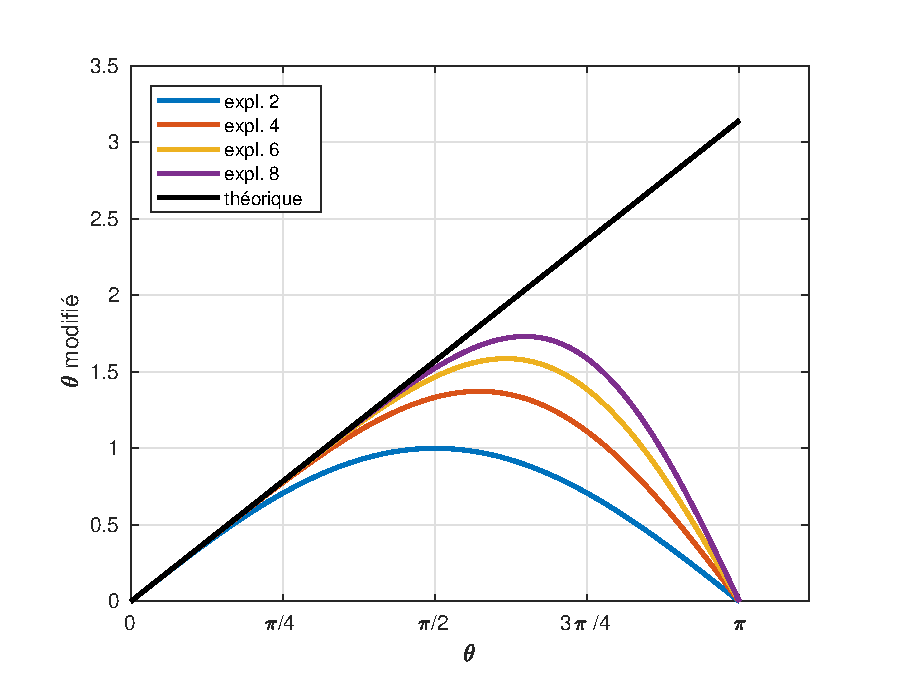
\includegraphics[scale=.6]{freq_classic.eps}
\end{center}
\caption{Représentation de $-i Q_{2J}\left( \exp(i \theta) \right)$ en fonction de $\theta$ pour les schémas d'approximation explicites $\delta_{x,2J}$ d'ordres $2J = 2$, $4$, $6$ et $8$.}
\label{fig:freq_classic}
\end{figure}

On s'intéresse à présent à la version matricielle de l'opérateur $\delta_{2J,x}$. On définit $D_{2J} \in \mathbb{M}_N(\mathbb{R})$ la matrice associée à l'opérateur $\delta_{2J,x}$ :
\begin{equation}
D_{2J} = \dfrac{1}{h} Q_{2J}(T).
\label{eq:matrice_explicite}
\end{equation}
pour toute fonction de grille $\mathfrak{u} \in l^2_{h,\per}$, la relation suivante est vérifiée
\begin{equation}
\vec(\delta_{2J,x} \mathfrak{u}) = D_{2J} \cdot \vec ( \mathfrak{u} ).
\end{equation}

\begin{itemize}
\item \textbf{Exemple 1 :} A l'ordre $2J=2$,  le schéma centré d'ordre 2 $\delta_x = \delta_{2,x}$ est associée à la matrice
\begin{equation}
D_2 = \dfrac{1}{2h}
\begin{bmatrix}
0 & 1 &   &   &   & -1 \\ 
-1 & 0 & 1 &   & (0) &   \\ 
  & -1 & 0 & 1 &   &   \\ 
  &   & \ddots & \ddots & \ddots &   \\ 
  & (0) &   & -1 & 0 & 1 \\ 
1 &   &   &   & -1 & 0
\end{bmatrix} 
\label{eq:matrice_D2}
\end{equation}

\item \textbf{Exemple 2 :} A l'ordre $2J=4$,  le schéma centré d'ordre 4 $\delta_{4,x}$ est associée à la matrice
\begin{equation}
D_4 = \dfrac{1}{2h}
\begin{bmatrix}
0 & 4/3 & -1/6 &   &   &   & 1/6 & -4/3 \\ 
-4/3 & 0 & 4/3 & -1/6 &   &   &   & 1/6 \\ 
1/6 & -4/3 & 0 & 4/3 & -1/6 &  & (0) &   \\ 
  & 1/6 & -4/3 & 0 & 4/3 & -1/6 &   &   \\ 
  &   & \ddots & \ddots & \ddots & \ddots & \ddots &   \\ 
  &  (0)& & 1/6 & -4/3 & 0 & 4/3 & -1/6 \\ 
-1/6 &   &   &   & 1/6 & -4/3 & 0 & 4/3 \\ 
4/3 & -1/6 &   &   &   & 1/6 & -4/3 & 0
\end{bmatrix}.
\end{equation}
\end{itemize}

Les propriétés spectrales de $D_{2J}$ se déduisent de celles de $\delta_{2J,x}$ vues dans la proposition \ref{prop:delta_x_spectre}.
\begin{proposition}
Les valeurs propres de $D_{2J}$ sont les valeurs 
\begin{equation}
\dfrac{1}{h}Q_{2J}(\omega^k) \text{ avec }-N/2 +1 \leq k \leq N/2,
\end{equation}
l'espace propre associé est $\Vect (U^k)$ avec $U^k = \vec (\mathfrak{u}^k)$.
\end{proposition}
De plus, on note la propriété de symétrie de $D_{2J}$ :
\begin{proposition}
La matrice $D_{2J}$ est antisymétrique.
\end{proposition}

\begin{proof}
Montrons que $D_{2J}^T = - D_{2J}$ :
\begin{align*}
D_{2J}^T & = \dfrac{1}{h} Q_{2J}(T)^T \\
	& = \dfrac{1}{h} \left( \gsum_{p=1}^J \dfrac{a_j}{2p} (T^p - T^{N-p}) \right)^T\\
	& = \dfrac{1}{h}\gsum_{p=1}^P \dfrac{a_p}{2p} ((T^p)^T - (T^{N-p})^T) \\
	& = \dfrac{1}{h}\gsum_{p=1}^J \dfrac{a_p}{2p} (T^{N-p} - T^{p}) \\
	& = - \dfrac{1}{h} \gsum_{p=1}^J \dfrac{a_p}{2p} (T^p - T^{N-p}) \\
	& = - D_{2J}
\end{align*}
d'où le résultat.
\end{proof}




























\subsection{Opérateurs Hermitiens périodiques 1D}

Dans ce travail, nous n'utilisons pas de schémas de la forme \eqref{eq:explicite_dx}. Les schémas hermitiens \cite{Lele1991} donnent de meilleurs résultats en ce qui concerne l'analyse fréquentielle. Ils sont couramment utilisés sur la résolution d'équations hyperboliques \cite{Chu1998} et permettent de bons résultats pour la capture des chocs \cite{Jiang2001}. De bons résultats ont aussi été donnés pour l'approximation de la dérivée seconde \cite{Abbas2011, Keller1971} ou en mécanique des fluides \cite{BenArtzi2005, BenArtzi2013}. Dans ce travail, nous ne considérons que les schémas à 3 points implicites pour lesquels nous souhaitons optimiser l'ordre de convergence. D'autres travaux vise à minimiser d'autres formes d'erreurs \cite{Kim1996, Kim2007}. Nous définissons l'opérateur $\sigma_{x}$ par :

\begin{equation}
(\sigma_{x} \mathfrak{u})_j = (1-2\beta) \mathfrak{u}_j + \beta \left( \mathfrak{u}_{j+1} + \mathfrak{u}_{j-1} \right) \text{ avec } 0 \leq j \leq N-1.
\end{equation}
On considère que l'opérateur $\delta_x$ est de la forme \eqref{eq:explicite_dx}, c'est à dire
\begin{equation}
\delta_x = \gsum_{p=1}^J a_p \dfrac{\tau^p - \tau^{-p}}{2ph}.
\end{equation}

\begin{theoreme}
Soit $f : \Omega \rightarrow \mathbb{R}$ alors l'identité discrète
\begin{equation}
\delta_{x} \mathfrak{u} = f^*
\end{equation}
est consistante à l'ordre $2J+2$ avec 
\begin{equation}
\partial_x u = f
\end{equation}
(avec $R_h = \sigma_x$ et $L_h = \delta_{x}$) si et seulement si les coefficients $(a_p)_{1 \leq p \leq J}$ et $\beta$ sont solution du système
\begin{equation}
\left\lbrace
\begin{array}{rcl}
\gsum_{p=1}^J a_p & = & 1 \\
\gsum_{p=1}^J a_p \dfrac{p^{2n}}{2n+1} & = & 2 \beta  \text{ pour } n=1,2,...J
\end{array}
\right.
\label{eq:hermitian_system}
\end{equation}
si $u$ est une fonction de $\mathcal{C}^{2J+3}$, alors pour tout $0 \leq j \leq N-1$, on a 
\begin{equation}
(\delta_{x} u^*)_j - (\sigma_{x} (\partial_x u)^*)_j = h^{2J+2} \left[ \dfrac{1}{(2J+3)!}  \left( \gsum_{p=1}^J a_p  p^{2J+2} \partial_x^{(2J+3)}u(\theta_p)\right)  - \left( \dfrac{2\beta}{(2J+2)!}    \partial_x^{(2J+3)}u(\rho_p)\right) \right]
\label{eq:eq_cons}
\end{equation} 
avec $\rho_p, \theta_p \in ]x_{j-p}, x_{j+p}[$.
\label{th:consistance_delta_x_implicite}
\end{theoreme}


\begin{proof}
Soit $u : x \in \Omega \mapsto u(x) \in \mathbb{R}$ une fonction de classe $\mathcal{C}^{2J+3}( \Omega)$ et $u^*$ la fonction de grille correspondante.
On considère les développements de Taylor :
\begin{equation}
\begin{array}{rcl}
u(x_j + ph) & = & u(x_j) + p h \partial_x u(x_j) + \cdots + \dfrac{(ph)^k}{k!}\partial_x^{(k)}u(x_j) + \cdots +\dfrac{(ph)^{2J+3}}{(2J+3)!} \partial_x^{(2J+3)}u(\xi)\\
u(x_j - ph) & = & u(x_j) - p h \partial_x u(x_j) + \cdots + \dfrac{(-ph)^k}{k!}\partial_x^{(k)} u(x_j) + \cdots +\dfrac{(-ph)^{2J+3}}{(2J+3)!} \partial_x^{(2J+3)}u(\eta)
\end{array}
\end{equation}
avec $\xi \in ]x_j, x_j+ph[$ et $\eta \in ]x_j-ph, x_j[$. En combinant ces deux égalités, on a
\begin{equation}
\dfrac{\tau_p u^*_j - \tau_{-p} u^*_j}{2ph} = \partial_x u(x_j) + \cdots + \dfrac{(ph)^{k-1}(1 - (-1)^k)}{2 \cdot k!} \partial_x^{(k)}u(x_j) + \cdots +\dfrac{(ph)^{2J+2}}{2(2J+3)!} \left( \partial_x^{(2J+3)}u(\xi) + \partial_x^{(2J+3)}u(\eta) \right)
\label{eq:preuve_herm1}
\end{equation}
D'autres part, on a 
\begin{multline}
(1-2\beta) \partial_x u^*_j + \beta \left( \tau_1 \partial_xu^*_{j} + \tau_{-1} \partial_xu^*_{j} \right) = \\
 \partial_x u^*_j +  \gsum_{k=1}^{2J+1} \beta \dfrac{h^{k}}{k!} \left( 1 + (-1)^k \right) \partial_x^{(k+1)}u(x_j)+ \beta \dfrac{h^{2J+2}}{(2J+2)!} \left(\partial_x^{(2J+3)}u(\varrho_p) + \partial_x^{(2J+3)}u(\sigma_p) \right) 
\label{eq:preuve_herm2}
\end{multline}
avec $\varrho_p \in ]x_j, x_j + ph[$ et $\sigma_p \in ]x_j - _h , x_j[$. 

On remarque directement que \eqref{eq:preuve_herm2} et $\gsum_{p=0}^J a_p  \eqref{eq:preuve_herm1}$ coïncident pour les puissances de $h$ impaires. 
Pour les autres valeurs, l'égalité est vrai si les coefficients $(a_p)_{1 \leq p \leq J}$ et $\beta$ sont solutions de \eqref{eq:hermitian_system}. L'erreur de troncature prend directement la forme 
\begin{multline}
(\delta_{x} u^*)_j - (\sigma_{x} \partial_x u^*)_j = \\
h^{2J+2} \left( \gsum_{p=1}^J a_p  \dfrac{p^{2J+2}}{2(2J+3)!} \left( \partial_x^{(2J+3)}u(\xi_p) + \partial_x^{(2J+3)}u(\eta_p) \right) - \dfrac{\beta}{(2J+2)!} \left(\partial_x^{(2J+3)}u(\varrho_p) + \partial_x^{(2J+3)}(\sigma_p) \right) \right).
\end{multline}
On conclut en utilisant le théorème des valeurs intermédiaires.
\end{proof}

Dans cette section, nous supposons que le système \eqref{eq:hermitian_system} admet une solution. Ce sera le cas pour tous les exemples considérés.

\begin{proposition}
Les valeurs propres de $\sigma_x$ sont
\begin{equation}
R(\omega^k) \text{ avec } R(X) = (1-2 \beta) + \beta(X+X^{N-1}) \in \mathbb{R}_{N-1}[X] \text{ et } -N/2+1 \leq k \leq N/2.
\end{equation}
avec $-N/2+1 \leq k \leq N/2$. L'espace propre associé est $\Vect ( \mathfrak{u}^k )$.
\end{proposition}

\begin{proof}
Il s'agit d'une conséquence de la proposition \ref{prop:eigen_Ptau} appliqué au polynôme $R$.
\end{proof}
Dans la suit, nous aurons besoin d'inverser l'opérateur $\sigma_x$. La propriété suivante permet de s'assurer de son inversibilité.
\begin{corollaire}
L'opérateur $\sigma_x$ est inversible si
\begin{equation}
| \beta | < \dfrac{1}{2}.
\end{equation}
\end{corollaire}

\begin{definition}
On suppose que $\beta$ et $(a_p)_{1 \leq p \leq J}$ sont solutions de \eqref{eq:hermitian_system} et que $|\beta| < 1/2$, on définit l'\textit{opérateur hermitien} d'approximation de la dérivée première $\delta_{2J+2,x}^H$ par 
\begin{equation}
\delta_{2J+2,x}^H = \sigma_x^{-1} \circ \delta_{x}.
\end{equation}
\label{def:herder}
\end{definition}

\begin{theoreme}
Si $u : x \in \Omega \mapsto u(x) \in \mathbb{R}$ est une fonction de classe $\mathcal{C}^{(2J+3)}$.
Alors 
\begin{equation}
\| (\partial_x u)^* - \delta_{2J+2,x}^H (u^*) \|_{\infty} \leq C h^{2J+2} \| \partial_x^{(2J+3)} u \|_{\infty}
\end{equation}
où $C$ est une constante indépendante de $u$ et de $h$.
\label{th:consistence_herm2}
\end{theoreme}

\begin{proof}
Par calcul immédiat, on a :
\begin{equation}
\begin{array}{rcl}
\|  (\partial_x u)^* - \delta_{2J+2,x}^H (u^*) \|_{\infty} &=& \| \sigma_{x}^{-1} \circ \left( \sigma_{x} u'^*  - \delta_{x}u^*\right) \|_{\infty}\\
                                      &\leq& \| \sigma_{x}^{-1} \|_{\infty} \| \sigma_{x} u'^*  - \delta_{x}u^*\|_{\infty}\\
                                      &\leq& C h^{2J+2}  \| \partial_x^{(2J+3)} u \|_{\infty}
\end{array}
\end{equation}
en utilisant $\sigma_{x}$ inversible et l'équation \eqref{eq:eq_cons}.
\end{proof}
Quelques exemples de schémas hermitiens sont donnés dans le corollaire suivant.

\textbf{Exemples : }
Soit $u : x \in \Omega \mapsto u(x) \in \mathbb{R}$ périodique alors 
\begin{itemize}
\item Si $u \in \mathcal{C}^{5}(\Omega)$ alors 
\begin{equation}
\left\lbrace
\begin{array}{rcl}
\sigma_{x} &=& \dfrac{4}{6} \Id + \dfrac{1}{6} \left( \tau_1 + \tau_{-1} \right)\\
\delta_{x} &=& \dfrac{\tau_1 - \tau_{-1}}{2h} \\ 
\end{array}
\right.
\label{eq:comp4}
\end{equation}
et $\delta^H_{4,x} = \sigma_x^{-1} \circ \delta_{x}$ définit un opérateur d'approximation de la dérivée première à l'ordre 4. En particulier, comme $\| \sigma_x^{-1} \|_{\infty} \leq 3$, on montre à partir de la proposition \ref{prop:eq_deltax2_sigmax} que :
\begin{equation}
\| (\partial_x u )^* - \delta_{4,x}^H (u^*) \|_{\infty} \leq \dfrac{h^4}{15} \| \partial_x^{(4)} i \|_{\infty}.
\label{eq:constante_err_derherm4}
\end{equation}

\item Si $u \in \mathcal{C}^{7}(\Omega)$ alors 
\begin{equation}
\left\lbrace
\begin{array}{rcl}
\sigma_{x} &=& \dfrac{1}{2} \Id + \dfrac{1}{4}\left( \tau_1 + \tau_{-1} \right) \\
\delta_{x} &=& \dfrac{5}{6} \dfrac{\tau_1 - \tau_{-1}}{2h} + \dfrac{1}{6} \dfrac{\tau_2 - \tau_{-2}}{4h}\\ 
\end{array}
\right.
\label{eq:comp6}
\end{equation}
et $\delta^H_{x} = \sigma_{x}^{-1} \circ \delta_{4,x}$ définit un opérateur d'approximation de la dérivée première à l'ordre 6,


\item Si $u \in \mathcal{C}^{9}(\Omega)$ alors 
\begin{equation}
\left\lbrace
\begin{array}{rcl}
\sigma_{x} &=& \dfrac{4}{7} \Id + \dfrac{3}{14}\left( \tau_1 + \tau_{-1} \right) \\
\delta_{x} &=& \dfrac{25}{28} \dfrac{\tau_1 - \tau_{-1}}{2h} + \dfrac{4}{35} \dfrac{\tau_2 - \tau_{-2}}{4h} - \dfrac{1}{140} \dfrac{\tau_3 - \tau_{-3}}{6h} \\ 
\end{array}
\right.
\label{eq:comp8}
\end{equation}
et $\delta^H_{8,x} = \sigma_{x}^{-1} \circ \delta_{x}$ définit un opérateur d'approximation de la dérivée première à l'ordre 8.
\end{itemize}


Les opérateurs $\sigma_x$ et $\delta_{x}$ s’expriment en fonction de $\tau$ donc ils commutent, tout comme $\sigma_x^{-1}$ et $\delta_{x}$:
\begin{equation}
\delta_{2J+2,x}^H = \sigma_x^{-1} \circ \delta_{x} = \delta_{x} \circ \sigma_x^{-1}.
\end{equation}
Notons la fraction rationnele $Q_{2J+2}^H \in \mathbb{R}(X)$ telle que 
\begin{equation}
Q_{2J+2}^H(X) = \dfrac{Q_{2J}(X)}{R(X)} = \dfrac{\gsum_{p=1}^J \dfrac{a_p}{2p} (X^p - X^{N-p})}{(1-2\beta) + \beta ( X + X^{N-1})}.
\label{eq:pol_hermitien}
\end{equation}
\begin{itemize}
\item \textbf{Exemple 1 :} $Q_4^H(X)$ est donné par
\begin{equation}
Q_4^H(X) = \dfrac{X-X^{N-1}}{\dfrac{4}{3} + \dfrac{1}{3}(X+X^{N-1})},
\label{eq:polhermi4}
\end{equation}
\item \textbf{Exemple 2 :} $Q_6^H(X)$ est donné par
\begin{equation}
Q_6^H(X) = \dfrac{\dfrac{5}{12}(X-X^{N-1}) + \dfrac{1}{24}(X^2-X^{N-2})}{\dfrac{1}{2} + \dfrac{1}{4}(X+X^{N-1})},
\end{equation}
\item \textbf{Exemple 3 :} $Q_8^H(X)$ est donné par
\begin{equation}
Q_8^H(X) = \dfrac{\dfrac{25}{56}(X-X^{N-1}) + \dfrac{4}{140}(X^2-X^{N-2}) - \dfrac{1}{840}(X^3-X^{N-3})}{\dfrac{4}{7} + \dfrac{3}{14}(X+X^{N-1})}.
\end{equation}
\end{itemize}

La fraction rationnelle $Q_{2J+2}^H$ permet d'exprimer $\delta_{2J+2,x}^H$ en fonction de $\tau$
\begin{equation}
\delta_{2J+2,x}^H = \dfrac{1}{h} Q_{2J+2}^H(\tau).
\end{equation}
L'opérateur $\delta_{2J+2,x}^H$ agit sur les fonctions de $l^2_{h,\per}$. Les propriétés spectrales de $\delta_{2J,x}^H$ s'expriment à l'aide de la fraction rationnelle $Q_{2J+2}^H$.

\begin{proposition}
Les valeurs propres de $\delta_{2J+2,x}^H$ sont 
\begin{equation}
\dfrac{1}{h} Q_{2J+2}^H (\omega^k)
\end{equation}
où $-N/2+1 \leq k \leq N/2$. L'espace propre associé à $\dfrac{1}{h} Q_{2J+2}^H (\omega^k)$ est donné par $\Vect( \mathfrak{u}^k )$.
\label{prop:eigen_mat_hermitien}
\end{proposition}

\begin{proposition}
Si les coefficient $(a_p)_{1 \leq p \leq J}$ et $\beta$ sont solutions du système \eqref{eq:hermitian_system}. Alors pour $-N/2+1  \leq k \leq N/2$ et $h=L/N$ on a
\begin{equation}
\dfrac{2 i \pi k}{N} - Q_{2J+2}^H \left( \exp \left( \dfrac{2 i \pi k}{N} \right) \right) = \mathcal{O}(h^{2J+3}).
\end{equation}
De plus, en posant $\theta = 2 k \pi / N$, on a
\begin{equation}
- i Q_{2J+2}^H(\exp (i \theta) ) = \dfrac{\sin(\theta)}{1 +2 \beta (\cos (\theta) -1)} \gsum_{p=1}^J \dfrac{a_p}{p} U_p (\cos \theta ) 
\end{equation}
où $(U_p)_{1 \leq p \leq J}$ désigne des polynômes de Tchebychev de seconde espèce.
\label{prop:hermitien_polynome}
\end{proposition}

\begin{proof}
D'une part, d'après le théorème \ref{th:consistance_delta_x_implicite} on a
\begin{equation}
\sigma_x (\partial_x u^k)^* - \delta_{x}(u^k)^* = \mathcal{O}(h^{2J+2}),
\end{equation}
donc en inversant l'opérateur $\sigma_x$, on a
\begin{equation}
(\partial_x u^k)^* - \delta_{2J+2,x}^H(u^k)^* = \mathcal{O}(h^{2J+2}).
\end{equation}
D'autres part, on rappelle que la fonction $u^k$ et la fonction de grille $\mathfrak{u}^k$ sont liées par
\begin{equation}
u^k = \sqrt{h} \mathfrak{u}^k,
\end{equation}
donc on a directement 
\begin{align*}
(\partial_x u^k)^* - \delta_{2J+2,x}^H (u^k)^* & = \dfrac{2 i \pi k}{L}(u^k)^* - \dfrac{1}{h}Q_{2J+2}^H(\omega^k) (u^k)^* \\
	& = \dfrac{1}{h} \left( \dfrac{2 i \pi h k}{L} - Q_{2J+2}^H(\omega^k) \right) (u^k)^*\\
	& = \dfrac{1}{h} \left( \dfrac{2 i \pi k}{N} - Q_{2J+2}^H \left( \exp \left( \dfrac{2 i \pi k}{N} \right) \right) \right) (u^k)^* .
\end{align*}
La fonction $u^k$ est bornée, donc
\begin{equation}
\dfrac{2 i \pi k}{N} - Q_{2J+2}^H \left( \exp \left( \dfrac{2 i \pi k}{N} \right) \right) = \mathcal{O}(h^{2J+1}).
\end{equation}
De plus par construction on a
\begin{align*}
Q_{2J} \left( \exp ( i \theta ) \right) & = \gsum_{p=1}^J a_p \dfrac{\exp ( i p \theta ) - \exp ( i (N-p) \theta )}{2 p} \text{par périodicité des opérateurs.} \\
	& = \gsum_{p=1}^J a_p \dfrac{\exp ( i p \theta ) - \exp ( -i p \theta )}{2 p} \\
	& = \gsum_{p=1}^J a_p \dfrac{i \sin (p \theta )}{p} \cos ( p \theta)\\
	& = i \dfrac{\sin(\theta)}{1 +2 \beta (\cos (\theta) -1)} \gsum_{p=1}^J \dfrac{a_p}{p} U_p (\cos \theta) \in i \mathbb{R}
\end{align*}
où $U_p$ désigne un polynôme de Tchebychev de seconde espèce.
De plus, on a $\sin (0 ) = \sin (\pi) = 0$, donc 
\begin{equation}
Q_{2J} \left( \exp ( i 0 ) \right) = Q_{2J} \left( \exp ( i \pi ) \right) = 0,
\end{equation}
ce qui conclut la proposition.
\end{proof}

Par $2 \pi$-périodicité et imparité de $\theta \in \mathbb{R} \mapsto - i Q_{2J+2}^H(e^{i \theta})$, et d'après la proposition \ref{prop:hermitien_polynome}, on souhaite comparer $\theta \in \mathbb{R} \mapsto - i Q_{2J+2}^H(e^{i \theta})$ et $\theta \in \mathbb{R} \mapsto \theta$. Quelques exemples, pour les valeurs de $2J+2 = 4$, $6$ et $8$, sont tracés dans la figure \ref{fig:freq_herm}. On compare ces fonctions avec celles obtenues pour les schémas $\delta_{2J,x}$ aux ordre 2, 4, 6 et 8. On constate que les schémas hermitiens $\delta_{2J+2,x}^H$ représentent mieux $\theta$ que les schémas $\delta_{2J,x}$. La représentation spectrale de la dérivée est meilleure en utilisant le schéma $\delta_{2J+2,x}^H$ que le schéma $\delta_{2J,x}$. De plus, plus l'ordre du schéma est élevé, mieux la fonction $\theta \in \mathbb{R} \mapsto \theta$ est approchée.

\begin{figure}[htbp]
\begin{center}
\includegraphics[scale=.6]{compact_freq.png}
\end{center}
\caption{Représentation de $-i Q_{2J+2}^H \left( e^{i \theta} \right)$ en fonction de $\theta$ pour les schémas d'approximation hermitien $\delta_{2J+2,x}^H$ d'ordres 2, 4, 6 et 8. Les courbes en pointillés représentent les fonctions $-i Q_{2J}\left( e^{i \theta} \right)$ associées aux opérateurs d'approximations $\delta_{2J,x}$.}
\label{fig:freq_herm}
\end{figure}


Considérons à présent la version matricielle de l'opérateur $\delta_{2J+2,x}^H$. On pose $P_{\sigma} \in \mathbb{M}_N(\mathbb{R})$ la matrice associée à l'opérateur $\sigma_x$. Cette matrice s'exprime par
\begin{align}
P_{\sigma} & = R(T) \\
  & = \begin{bmatrix}
  1 - 2 \beta & \beta &   &   & \beta \\ 
  \beta & 1 - 2 \beta & \beta & (0) &   \\ 
    & \ddots & \ddots & \ddots &   \\ 
    & (0) & \beta & 1 - 2 \beta & \beta \\ 
  \beta &   &   & \beta & 1 - 2 \beta
  \end{bmatrix} \in \mathbb{M}_{N}(\mathbb{R}).
\label{eq:matrice_implicitpart}
\end{align}
La relation suivante est immédiate
\begin{equation}
\vec (\sigma_x \mathfrak{u}) = P_{\sigma} \cdot \vec (\mathfrak{u}).
\end{equation}
Les valeurs propres de $P_{\sigma}$ sont connues et données par le corollaire \ref{cor:eigen_P(T)}.
\begin{proposition}
Les valeurs propres de $P_{\sigma}$ sont 
\begin{equation}
R(\omega^k)
\end{equation}
avec $-N/2+1 \leq k \leq N/2$. L'espace propre associé à $R(\omega^k)$ est $\Vect(U^k)$ avec $U^k = \vec( \mathfrak{u}^k )$.
\end{proposition}

$P_{\sigma}$ est inversible si $|\beta |<1/4$ et trivialement symétrique. 
De la même manière, on a déjà vu que 
\begin{equation}
D_{2J} = \dfrac{1}{h} Q_{2J}(T) \in \mathbb{M}_{N}(\mathbb{R})
\end{equation}
donc 
\begin{equation}
\vec (\delta_{x} \mathfrak{u}) = D_{2J} \cdot \vec (\mathfrak{u}).
\label{eq:systhermitien}
\end{equation}
Le calcul de $\delta^H_{2J+2,x} \mathfrak{u}$ se fait par la résolution du système
\begin{equation}
P_{\sigma} \cdot \vec (\delta_{2J+2,x}^H \mathfrak{u}) = D_{2J} \cdot \vec (\mathfrak{u})
\end{equation}
et on a 
\begin{equation}
\vec (\delta_{2J+2,x} \mathfrak{u} ) =P_{\sigma}^{-1} D_{2J} \cdot \vec (\mathfrak{u}).
\end{equation}

\begin{proposition}
Les matrices $D_{2J}$, $P_{\sigma}$ et $P^{-1}_{\sigma}$ commutent.
\end{proposition}

\begin{proof}
Les matrices $D_{2J}$ et $P_{\sigma}$ s'expriment en fonction de $T$ d'où la propriété.
\end{proof}

\begin{proposition}
La matrice $P^{-1}_{\sigma}D_{2J}$ est antisymétrique.
\label{prop:derhermi_antisym}
\end{proposition}

\begin{proof}
Par calcul immédiat, on a :
\begin{equation}
(P^{-1}_{\sigma}D_{2J})^T = D_{2J}^T P_{\sigma}^{-T} = - D_{2J} P_{\sigma}^{-1} = - P_{\sigma}^{-1} D_{2J}.
\end{equation}
car $D_{2J}$ est antisymétrique et $P_{\sigma}$ est symétrique (donc $P^{-1}_{\sigma}$ aussi). 
\end{proof}

Le calcul de $\delta_{2J+2,x}^H \mathfrak{u}$ se fait par résolution d'un système linéaire. Ce système peut être résolu grâce à la formule de Shermann-Morisson-Woodbury couplé à un solveur tridiagonal comme l'algorithme de Thomas ou grâce à un solveur basé sur la transformée de Fourier rapide.

\begin{proposition}
\textbf{(Formule de Shermann-Morisson-Woodbury)} Soient $A, B \in \mathbb{M}_N \left(\mathbb{R} \right)$ deux matrices inversibles telles que 
\begin{equation}
A = B + R S^T,
\end{equation}
avec $R$ et $S$ deux matrices de $\mathbb{M}_{N,n} \left(\mathbb{R} \right)$ avec $n \leq N$.
Alors l'inverse de $A$ peut s'écrire
\begin{equation}
A^{-1} = B^{-1} - B^{-1} R \left( Id + S^T B^{-1} R  \right)^{-1} S^T B^{-1}.
\label{eq:SMW}
\end{equation}
\end{proposition}

\begin{proof}
Il suffit de vérifier que 
\begin{equation}
\left( B + R S^T \right) \left( B^{-1} - B^{-1} R \left( Id + S^T B^{-1} R  \right)^{-1} S^T B^{-1} \right) = Id.
\end{equation}
\end{proof}

Dans le cas où $n \lll N$, $A$ est une petite perturbation de la matrice $B$ de la forme 
\begin{equation}
A = B + \delta B
\end{equation}
avec $\rang  (\delta B) $ "petit". Si on peut facilement calculer l'inverse de $B$ la formule de Shermann-Morisson-Woodbury \eqref{eq:SMW} donne un algorithme efficace de résolution du système
\begin{equation}
A X = b.
\end{equation} 

\begin{center}
\begin{minipage}[H]{12cm}
  \begin{algorithm}[H]
    \caption{: Algorithme de Shermann-Morisson-Woodbury}\label{alg:SMW}
    \begin{algorithmic}[1]
	\State Calcul de $V_1 = B^{-1} b$,
	\State Calcul de $V_2 = S^T V_1$,
	\State Calcul de $V_3 = (Id + S^T B^{-1}R)^{-1} V_2$ (résolution d'un système de petite taille),
	\State Calcul de $V_4 = R V_3$,
	\State Calcul de $V_5 = B^{-1} V_4$,
	\State Calcul de $X = V_1 - V_5$.
    \end{algorithmic}
    \end{algorithm}
\end{minipage}
\end{center}

\begin{proposition}
Soit $P_{\sigma}$ et $\tilde{P}_{\sigma}$ les matrice donnée par 
\begin{equation}
P_{\sigma} = \begin{bmatrix}
  1 - 2 \beta & \beta &   &   & \beta \\ 
  \beta & 1 - 2 \beta & \beta & (0) &   \\ 
    & \ddots & \ddots & \ddots &   \\ 
    & (0) & \beta & 1 - 2 \beta & \beta \\ 
  \beta &   &   & \beta & 1 - 2 \beta
  \end{bmatrix}  \text{ et }
\tilde{P}_{\sigma} = 
\begin{bmatrix}
  1 - 2 \beta & \beta &   &   &  \\ 
  \beta & 1 - 2 \beta & \beta & (0) &   \\ 
    & \ddots & \ddots & \ddots &   \\ 
    & (0) & \beta & 1 - 2 \beta & \beta \\ 
   &   &   & \beta & 1 - 2 \beta
  \end{bmatrix} .
\end{equation}
Alors 
\begin{equation}
P_{\sigma} = \tilde{P}_{\sigma} + R S^T
\end{equation} 
avec 
\begin{equation}
R = \dfrac{1}{6}\begin{bmatrix}
1 & 0 \\ 
0 & \vdots \\ 
\vdots & \vdots \\ 
\vdots & 0 \\ 
0 & 1
\end{bmatrix} \text{ et } 
S = \begin{bmatrix}
0 & 1 \\ 
\vdots & 0 \\ 
\vdots & \vdots \\ 
0 & \vdots \\ 
1 & 0
\end{bmatrix} 
\end{equation}
\end{proposition}

Il découle l'algorithme le calcul de $\vec (\delta_{2J+2,x}^H \mathfrak{u}) = P^{-1}_{\sigma} D_{2J} \cdot \vec (\mathfrak{u})$ donné par

\begin{center}
\begin{minipage}[H]{12cm}
  \begin{algorithm}[H]
    \caption{: Calcul Hermitien}\label{alg:SH}
    \begin{algorithmic}[1]
    \State Calcul de $b = D_{2J} \vec (\mathfrak{u})$,
	\State Calcul de $V_1 = \tilde{P}_{\sigma}^{-1} b$,
	\State Calcul de $V_2 = S^T V_1$,
	\State Calcul de $V_3 = (Id + S^T \tilde{P}_{\sigma}^{-1}R)^{-1} V_2$ (résolution d'un système de taille $2 \times 2$),
	\State Calcul de $V_4 = R V_3$,
	\State Calcul de $V_5 = \tilde{P}_{\sigma}^{-1} V_4$,
	\State Calcul de $\vec (\delta_{2J+2,x}^H \mathfrak{u}) = V_1 - V_5$.
    \end{algorithmic}
    \end{algorithm}
\end{minipage}
\end{center}

L'utilisation de l'algorithme \ref{alg:SH} pour la résolution du système \eqref{eq:systhermitien} permet de se ramener à la résolution d'un système tridiagonal. La résolution se fait en utilisant l'algorithme de Thomas \cite{Conte2017,Quarteroni2010}. Le coût global de l'algorithme de résolution est alors $\mathcal{O}(N)$. On aurait aussi pu utiliser un solveur rapide de type transformée de Fourier rapide \cite{VanLoan1992}. Mais le coût en calcul d'un tel algorithme est de l'ordre de $\mathcal{O}(N \log (N))$, ce qui est plus élevé.























\subsection{Opérateur de filtrage}

Pour améliorer les propriétés de stabilité d'un schéma centré en espace, il est connu que l'utilisation d'un opérateur de type "filtrage", à chaque pas de temps, est bénéfique. Un opérateur de type filtrage est un opérateur de la forme
\begin{equation}
\mathcal{F}_{2J,x} = \gsum_{p=0}^J a_p \dfrac{\tau^p + \tau^{-p}}{2}
\label{eq:ftr}
\end{equation}
pour $\mathfrak{u} \in l^2_{h,\per}$ fonction de grille périodique, on a
\begin{equation}
\mathcal{F}_{2J,x} (\mathfrak{u} )_j = \gsum_{p=0}^J a_p \dfrac{\mathfrak{u}_{j+p} + \mathfrak{u}_{j-p}}{2} \text{ avec } 0  \leq j \leq N-1.
\end{equation}
Soit $S_{2J} \in \mathbb{R}_{N-1}[X]$ définit par 
\begin{equation}
S_{2J}(X) = \gsum_{p=0}^J a_p \dfrac{X^p + X^{N-p}}{2},
\label{eq:pol_filtrage}
\end{equation}
on a $\mathcal{F}_{2J,x}(\mathfrak{u})_j = S_{2J}(\tau)(\mathfrak{u})_j$ pour tout $0 \leq j \leq N-1$.

L'opérateur $\mathcal{F}_{2J,x}$ est un opérateur d'interpolation au sens de la définition \ref{def:consistance}. C'est à dire qu'il est consistant avec l'identité.
D'autres part, il joue le rôle d'une dissipation numérique. Cette contrainte se traduit par le fait que $\mathfrak{u}^{N/2}$, qui vérifie
\begin{equation}
\mathfrak{u}^{N/2}_j = (-1)^j \text{ pour } 0 \leq j \leq N-1,
\end{equation}
est inclus dans le noyaux de $\mathcal{F}_{2J,x}$ : $\mathcal{F}_{2J,x}(\mathfrak{u}^{N/2}) = \mathfrak{0}$. On note que l'on a alors
\begin{equation}
\ker (\mathcal{F}_{2J,x} ) \subset \ker (\delta_{2J,x} ) \text{ et } \ker (\mathcal{F}_{2J,x} ) \subset \ker (\delta_{2J,x}^H ).
\end{equation}
En pratique, cela correspond au mode oscillant à la fréquence du maillage. A chaque itération en temps, on souhaite supprimer ce mode en projetant la solution sur l'orthogonal du mode oscillant :
\begin{equation}
\Vect (\mathfrak{u}^{N/2})^{\perp}.
\end{equation}
De plus, un opérateur de filtrage doit laisser $\mathfrak{u}^0$ inchangé, c'est à dire
\begin{equation}
\mathcal{F}_{2J,x}(\mathfrak{u}^{0}) = \mathfrak{u}^{0}.
\end{equation}
Comme $\mathfrak{u}^0_j = 1$ pour $0 \leq j \leq N-1$, cette condition correspond à avoir
\begin{equation}
\mathcal{F}_{2J,x}(\mathfrak{u}^{0}) = \gsum_{p=0}^J a_p = 1.
\end{equation}
Nous nous concentrons sur les filtres maximisant l'ordre de précision \cite{Redonnet2001} et perturbant les données le moins possible. D'autres filtres visent à minimiser la perturbation \cite{Bogey2004}. Dans ce cadre, nous définissons l'opérateur de filtrage par 

\begin{definition}
L'opérateur $\mathcal{F}_{2J,x}$ est appelé filtre centré s'il s'agit d'un opérateur aux différences finies de la forme \eqref{eq:ftr} et si les coefficients $(a_p)_{1 \leq p \leq J}$ vérifient :
\begin{itemize}
\item Consistance du filtrage :
\begin{equation}
\gsum_{p=0}^J a_p = 1,
\label{eq:ftr_consistance}
\end{equation}
\item Suppression du mode $\mathfrak{u}^{N/2}$ :
\begin{equation}
\gsum_{p=0}^J a_p (-1)^p = 0,
\label{eq:ftr_filtrage}
\end{equation}
\item Précision de l'opérateur
\begin{equation}
\gsum_{p=0}^J a_p p^{2k} = 0 \text{ pour } 1 \leq k \leq J-1.
\label{eq:ftr_precision}
\end{equation}
\end{itemize}
\end{definition}

\begin{figure}[htbp]
\begin{center}
\begin{tikzpicture}[scale=1.4]
	\draw (-4,1) -- (-3,-1) ;
	\draw (-3,-1) -- (-2,1) ;
	\draw (-2,1) -- (-1,-1) ;
	\draw (-1,-1) -- (0,1) ;
	\draw (0,1) -- (1,-1) ;
	\draw (1,-1) -- (2,1) ;
	\draw (2,1) -- (3,-1) ;
	\draw (3,-1) -- (4,1) ;
	
	\draw (4,0) -- (-4,0) ;
	\foreach \k in {-3,...,3}
		{\draw  (\k,0) node[color=blue] {$\bullet$} ;
	   	\draw (\k,0) node {$\circ$} ;
	   	}
\end{tikzpicture}
\end{center}
\caption{Représentation graphique du monde $\mathfrak{u}^{N/2} \in l^2_{h,\per}$.}
\label{fig:hf_waves}
\end{figure}

\begin{proposition}
Si les $J$ coefficients $(a_p)_{1 \leq p \leq J}$ vérifient \eqref{eq:ftr_consistance}, \eqref{eq:ftr_filtrage} et \eqref{eq:ftr_precision}, c'est a dire
\begin{equation}
\left\lbrace
\begin{array}{rcl}
\gsum_{p=0}^J a_p & = & 1 \\
\gsum_{p=0}^J a_p (-1)^p & = & 0 \\
\gsum_{p=0}^J a_p p^{2k} & = & 0 \text{ avec } 1 \leq k \leq J-1,
\end{array}
\right.
\label{eq:system_ftr}
\end{equation}
alors l'opérateur de filtrage $\mathcal{F}_{x,2J}$ est consistant avec l'identité.

Soit $u$ une fonction régulière et $u^*$ la fonction de grille associée. L'erreur de troncature de l'opérateur de filtrage $\mathcal{F}_{x,2J}$ est donnée par
\begin{equation}
\mathcal{F}_{x,2J}(u^*)_j - u^*_j = \dfrac{h^{2J}}{(2J)!} \left( \gsum_{p=1}^J a_p p^{2J} \partial_x^{(2J)}u(\alpha_p) \right)
\end{equation}
avec $\alpha_p \in ]x_{j-p}, x_{j+p}[$.
\label{prop:filter_def}
\end{proposition}

\begin{proof}
$u$ est une fonction régulière, donc d'après la formule de Taylor-Lagrange il existe $\xi \in ]x,x+h[$ tel que
\begin{equation}
u(x+h) = \gsum_{k=0}^{2J-1} \dfrac{h^k}{k!} \partial_x^{(k)} u(x) +\dfrac{1}{(2J)!} \partial_x^{(2J)}u(\xi).
\end{equation}
D'après cette formule et le théorème des valeurs intermédiaires, on a
\begin{align*}
\dfrac{\tau_p \mathfrak{u}_j + \tau_{-p} \mathfrak{u}_j}{2} & = \dfrac{u(x_j + ph) - u(x_j-ph)}{2} \\
& = \gsum_{k=0}^{2J-1} \dfrac{h^k + (-h)^k}{2k!} \partial_x^{(k)}u(x_j) + \dfrac{h^{2J}}{(2J)!} \partial_x^{(2J)} u(\alpha_p)
\end{align*}
avec $\alpha_p \in ]x_j - ph, x_j + ph[$. Alors en multipliant cette relation par $a_p$ et en sommant sur $p$, on obtient :
\begin{align*}
\gsum_{p=1}^J a_p \dfrac{\tau_p \mathfrak{u}_j + \tau_{-p} \mathfrak{u}_j}{2} & = \gsum_{p=1}^J \gsum_{k=0}^{2J-1} a_p \dfrac{(ph)^k + (-ph)^k}{2k!} \partial_x^{(k)}u(x_j) + \gsum_{p=1}^J a_p \dfrac{(ph)^{2J}}{(2J)!} \partial_x^{(2J)}u(\alpha_p) \\
& = \gsum_{k=0}^{2J-1} \dfrac{h^k}{2 (k!)} \left( \gsum_{p=0}^J (p^k + (-p)^k) \right) \partial_x^{(k)} u(x) + \gsum_{p=0}^J a_p \dfrac{(ph)^{2J}}{(2J)!} \partial_x^{(2J)}u(\alpha_p) \\
& = \underbrace{ \left( \gsum_{p=0}^J a_p \right)}_{=1}u(x_j) + 
\gsum_{k=1}^{2J-1} \dfrac{h^k}{2(k!)} \underbrace{\left( \gsum_{p=0}^J (p^k + (-p)^k)  \right)}_{=0 \text{ si } k \text{ impair.}} \partial_x^{(k)}u(x_j) + \dfrac{h^{2J}}{(2J)!} \gsum_{p=0}^Ja_p p^{2J} \partial_x^{(2J)}u(\alpha_p)  \\
& = u(x_j) + \gsum_{k=1}^J \dfrac{h^{2k}}{k!} \underbrace{\left( \gsum_{p=0}^J a_p p^{2k} \right)}_{ = 0 \text{ d'après \eqref{eq:ftr_precision}}}
+ \dfrac{h^{2J}}{(2J)!} \left( \gsum_{p=0}^J a_p p^{2J} \partial_x^{(2J)}u(\alpha_p) \right) \\
& = u(x_j) + \dfrac{h^{2J}}{(2J)!} \left( \gsum_{p=0}^J a_p p^{2J} \partial_x^{(2J)}u(\alpha_p) \right).
\end{align*}
On retrouve ainsi l'erreur de consistance souhaitée et le résultat est prouvé.
\end{proof}

\begin{corollaire}
Si les coefficients $(a_p)_{1 \leq p \leq J}$ sont solution de \eqref{eq:system_ftr} alors pour toute fonction $u$ régulière il existe $C>0$ indépendant de $h$ et de $u$ tel que  on a 
\begin{equation}
\| u^* -  \mathcal{F}_{x,2J}(u^*) \|_{\infty} \leq C h^{2J} \| (\partial_x^{(2J)}u)^* \|_{\infty}.
\end{equation}
\end{corollaire}

L'existence et l'unicité des opérateurs de filtrage $\mathcal{F}_{x,2J}$ est donnée par la proposition suivante :

\begin{proposition}
Le système \eqref{eq:system_ftr} admet une unique solution.
\end{proposition}

\begin{proof}
Le système \eqref{eq:system_ftr} s'écrit en matriciel :
\begin{equation}
\underbrace{\begin{bmatrix}
1 & 1 & 1 & 1 & \cdots & 1\\
1 & -1 & 1 & -1 & \cdots & (-1)^J\\
0 & 1 & 2^2 & 3^2 & \cdots & J^2 \\
0 & 1 & 2^4 & 3^4 & \cdots & J^4 \\
0 & 1 & 2^6 & 3^6 & \cdots & J^6 \\
\vdots & \vdots & \vdots & \vdots & \ddots & \vdots \\
0 & 1 & (2^2)^{J-1} & (3^2)^{J-1} & \cdots & (J^2)^{J-1}
\end{bmatrix}}_{= A}
\underbrace{\begin{bmatrix}
a_0 \\ a_1 \\ a_2 \\ a_3 \\ a_4 \\ \vdots \\ a_J
\end{bmatrix}
}_{=a} = \underbrace{\begin{bmatrix}
1 \\ 0 \\ 0 \\ 0 \\ 0 \\  \vdots \\ 0
\end{bmatrix}
}_{= b}.
\end{equation}
En remplaçant la deuxième ligne par une combinaison de la première et de la deuxième ligne : $L_2 \leftarrow L_1 - L_2$, on obtiens :
\begin{equation}
\underbrace{\begin{bmatrix}
1 & 1 & 1 & 1 & \cdots & 1\\
0 & 2 & 0 & 2 & \cdots & 1-(-1)^J\\
0 & 1 & 2^2 & 3^2 & \cdots & J^2 \\
0 & 1 & 2^4 & 3^4 & \cdots & J^4 \\
0 & 1 & 2^6 & 3^6 & \cdots & J^6 \\
\vdots & \vdots & \vdots & \vdots & \ddots & \vdots \\
0 & 1 & (2^2)^{J-1} & (3^2)^{J-1} & \cdots & (J^2)^{J-1}
\end{bmatrix}}_{= \tilde{A}}
\underbrace{\begin{bmatrix}
a_0 \\ a_1 \\ a_2 \\ a_3 \\ a_4 \\ \vdots \\ a_J
\end{bmatrix}
}_{=a} = \underbrace{\begin{bmatrix}
1 \\ 1 \\ 0 \\ 0 \\ 0 \\ \vdots \\ 0
\end{bmatrix}
}_{= \tilde{b}}.
\end{equation}
Pour montrer que le système \eqref{eq:system_ftr}, on montre que la matrice $\tilde{A} \in \mathbb{M}_J(\mathbb{R})$ est inversible. En effet :
\begin{align*}
\det (\tilde{A}) & = \begin{vmatrix}
1 & 1 & 1 & 1 & \cdots & 1\\
0 & 2 & 0 & 2 & \cdots & 1-(-1)^J\\
0 & 1 & 2^2 & 3^2 & \cdots & J^2 \\
0 & 1 & 2^4 & 3^4 & \cdots & J^4 \\
0 & 1 & 2^6 & 3^6 & \cdots & J^6 \\
\vdots & \vdots & \vdots & \vdots & \ddots & \vdots \\
0 & 1 & (2^2)^{J-1} & (3^2)^{J-1} & \cdots & (J^2)^{J-1}
\end{vmatrix} \\
& = \begin{vmatrix}
2 & 0 & 2 & \cdots & 1-(-1)^J\\
1 & 2^2 & 3^2 & \cdots & J^2 \\
1 & 2^4 & 3^4 & \cdots & J^4 \\
1 & 2^6 & 3^6 & \cdots & J^6 \\
\vdots & \vdots & \vdots & \ddots & \vdots \\
1 & (2^2)^{J-1} & (3^2)^{J-1} & \cdots & (J^2)^{J-1}
\end{vmatrix} \\
& = 2 \gsum_{p=0}^{\lfloor \frac{J-1}{2} \rfloor} \Delta_{2p+1}.
\end{align*}
On va montrer que pour tout $1 \leq p \leq J$, $\Delta_p >0$. Ainsi, $\det(\tilde{A})$ est la somme de nombres strictement positifs, donc $\det(\tilde{A})>0$. $\Delta_p$ est donné par
\begin{align*}
\Delta_p & = \begin{vmatrix}
1 & 2^2 & 3^2 & \cdots & (p-1)^2 & (p+1)^2 & \cdots & J^2 \\ 
1 & (2^2)^2 & (3^2)^2 & \cdots & ((p-1)^2)^2 & ((p+1)^2)^{2} & \cdots & (J^2)^2 \\ 
\vdots & \vdots & \vdots & \ddots & \vdots & \vdots & \ddots & \vdots \\ 
1 & (2^2)^{J-1} & (3^2)^{J-1} & \cdots & ((p-1)^2)^{J-1} & ((p+1)^2)^{J-1} & \cdots & (J^2)^{J-1}
\end{vmatrix} \\
& = \left( \dfrac{J!}{p} \right) \begin{vmatrix}
1 & 1^2 & 1^2 & \cdots & 1^2 & 1^2 & \cdots & 1^2 \\ 
1 & 2^2 & 3^2 & \cdots & (p-1)^2 & (p+1)^{2} & \cdots & J^2 \\ 
\vdots & \vdots & \vdots & \ddots & \vdots & \vdots & \ddots & \vdots \\ 
1 & (2^2)^{J-2} & (3^2)^{J-2} & \cdots & ((p-1)^2)^{J-2} & ((p+1)^2)^{J-2} & \cdots & (J^2)^{J-2}
\end{vmatrix} \\
& = \left( \dfrac{J!}{p} \right) \VDM(1, 2^2, 3^2, \cdots (p-1)^2, (p+1)^2, \cdots, J^2)
\end{align*}
Où $\VDM$ désigne un déterminant de Vandermonde \cite{Evans1976} déterminé par 
\begin{equation}
\VDM(\alpha_1, \cdots, \alpha_n) = \gprod_{1\leq i < j \leq n} (\alpha_j - \alpha_i).
\end{equation}
Dans notre cadre, on a
\begin{equation}
\Delta_p = \left( \dfrac{J!}{p} \right) \VDM(\alpha_1, \alpha_2, \cdots \alpha_{J-1})
\end{equation}
avec $\alpha_j$ donné par
\begin{equation}
\alpha_j = \left\lbrace
\begin{array}{cl}
j^2 & \text{ si } j<p \\
(j+1)^2 & \text{ si } j \geq p.
\end{array}
\right.
\end{equation}
Ainsi, si $j>i$, on observe que $\alpha_j - \alpha_i>0$, donc
\begin{align*}
\Delta_p & = \left( \dfrac{J!}{p} \right) \VDM(1, 2^2, 3^2, \cdots (p-1)^2, (p+1)^2, \cdots, J^2) \\
	& = \left( \dfrac{J!}{k} \right)  \gprod_{1\leq i < j \leq J-1} \underbrace{(\alpha_j - \alpha_i)}_{>0} >0.
\end{align*}
$\det(\tilde{A})$ est une somme de termes strictement positifs donc $\det(\tilde{A})>0$ et en particulier, $\det(\tilde{A}) \neq 0$ et le système admet une unique solution.
\end{proof}

\textbf{Exemples : } on donne les filtres pour $J=1$, $2$, $3$, $4$ ou $5$. 
\begin{itemize}
\item Soit $u \in \mathcal{C}^{2}(\Omega)$ alors
\begin{equation}
\mathcal{F}_{2,x} = \dfrac{1}{2} \Id + \dfrac{1}{2} \dfrac{\tau_1 + \tau_{-1}}{2}
\end{equation}
définit un opérateur de filtrage à l'ordre 2,

\item soit $u \in \mathcal{C}^{4}(\Omega)$ alors
\begin{equation}
\mathcal{F}_{4,x} = \dfrac{10}{16} \Id + \dfrac{8}{16} \dfrac{\tau_1 + \tau_{-1}}{2} - \dfrac{2}{16} \dfrac{\tau_2 + \tau_{-2}}{2}
\end{equation}
définit un opérateur de filtrage à l'ordre 4,

\item soit $u \in \mathcal{C}^{6}(\Omega)$ alors
\begin{equation}
\mathcal{F}_{6,x} = \dfrac{44}{64} \Id + \dfrac{30}{64} \dfrac{\tau_1 + \tau_{-1}}{2} - \dfrac{12}{64} \dfrac{\tau_2 + \tau_{-2}}{2} + \dfrac{2}{64} \dfrac{\tau_3 + \tau_{-3}}{2}
\end{equation}
définit un opérateur de filtrage à l'ordre 6,

\item soit $u \in \mathcal{C}^{8}(\Omega)$ alors
\begin{equation}
\mathcal{F}_{8,x} = \dfrac{186}{256} \Id + \dfrac{112}{256} \dfrac{\tau_1 + \tau_{-1}}{2} - \dfrac{56}{256} \dfrac{\tau_2 + \tau_{-2}}{2} + \dfrac{16}{256} \dfrac{\tau_3 + \tau_{-3}}{2} - \dfrac{2}{256} \dfrac{\tau_4 + \tau_{-4}}{2}
\end{equation}
définit un opérateur de filtrage à l'ordre 8,

\item soit $u \in \mathcal{C}^{10}(\Omega)$ alors
\begin{equation}
\mathcal{F}_{10,x} = \dfrac{772}{1024} \Id + \dfrac{420}{1024} \dfrac{\tau_1 + \tau_{-1}}{2} - \dfrac{240}{1024} \dfrac{\tau_2 + \tau_{-2}}{2} + \dfrac{90}{1024} \dfrac{\tau_3 + \tau_{-3}}{2} - \dfrac{20}{1024} \dfrac{\tau_4 + \tau_{-4}}{2} + \dfrac{2}{1024} \dfrac{\tau_5 + \tau_{-5}}{2}
\end{equation}
définit un opérateur de filtrage à l'ordre 10.
\end{itemize}

Quelques filtres particuliers sont donnés par la table \ref{tab:filter} en fonction de leur ordre de précision.
\begin{table}[htbp]
\begin{center}
\begin{tabular}{|c||cccccc|}
\hline
\textbf{Ordre de précision : }$\mathbf{2J}$ & $a_0$ & $a_1$ & $a_2$ & $a_3$ & $a_4$ & $a_5$ \\
\hline \hline
$2$ & $1/2$ & $1/2$ & & & & \\
\hline
$4$ & $10/16$ & $8/16$ & $-2/16$ & & & \\
\hline
$6$ & $44/64$ & $30/64$ & $-12/64$ & $2/64$ & & \\
\hline
$8$ & $186/256$ & $112/256$ & $-56/256$ & $16/256$ & $-2/256$ & \\
\hline
$10$ & $772/1024$ & $420/1024$ & $-240/1024$ & $90/1024$ & $-20/1024$ & $2/1024$ \\
\hline
\end{tabular}
\end{center}
\caption{Exemples de filtres de la forme \eqref{eq:ftr} et leurs ordres de précision.}
\label{tab:filter}
\end{table}

Les valeurs propres et fonctions propres de $\mathcal{F}_{x,2J}$ sont issus de la proposition \ref{prop:eigen_Ptau} appliqué au polynôme $S_{2J} \in \mathbb{R}_J [X]$ défini par \eqref{eq:pol_filtrage}.

\begin{proposition}
Les valeurs propres de $\mathcal{F}_{2J,x}$ sont 
\begin{equation}
S_{2J} (\omega^k)
\end{equation}
où $-N/2+1 \leq k \leq N/2$. L'espace propre associé à $S_{2J} (\omega^k)$ est donné par $\Vect( \mathfrak{u}^k )$.
\label{prop:eigen_filtre}
\end{proposition}

\begin{theoreme}
Soit $\beta : \theta \in [0, \pi] \mapsto \beta(\theta) = \gsum_{p=0}^J a_p \cos (p \theta)$ le \textit{symbole} de l'opérateur de filtrage $\mathcal{F}_{2J,x}$, alors
\begin{itemize}
\item il existe un unique polynome $P \in \mathbb{R}_{J}(X)$ tel que
\begin{equation}
\beta(\theta) = P(\cos (\theta)),
\end{equation}
ce polynome est déterminé par
\begin{equation}
P(X) = 1 - \dfrac{1}{2^J}(1-X)^J,
\end{equation}
\item Pour tout $\theta \in [0, \pi]$, on a
\begin{equation}
0 \leq \beta(\theta) \leq 1.
\end{equation}
\end{itemize}
\label{th:filtre_dissipatif}
\end{theoreme}

\begin{proof}
\begin{itemize}
\item Les polynômes de Tchebytchev, notés $T_p$ , de première espèce sont définis par
\begin{equation}
T_p(\cos (\theta)) = \cos (p \theta).
\end{equation}
On a $T_p \in \mathbb{R}_p[X]$ et les $T_p$ forment une suite de polynômes de degrés croissants. Ils forment une base de $\mathbb{R}_p[X]$ et on a
\begin{align*}
\beta(\theta) & = \gsum_{p=0}^J a_p \cos (p \theta) \\
	& = \gsum_{p=0}^J a_p T_p( \cos (\theta)),
\end{align*}
ainsi il existe un polynôme $P = \gsum_{p=0}^J a_p T_p$ de degré $J$ tel que
\begin{equation}
\beta(\theta) = P(\cos (\theta)).
\end{equation}
Comme les polynômes $(T_p)_{0 \leq p \leq J}$ forment une base de $\mathbb{R}_{J}[X]$, ce polynôme est unique.

Les fonctions $\theta \mapsto \cos (n \theta)$ forment une famille libre pour $0 \leq n \leq J$. On pose $E_J$ l'espace engendré par ces fonctions, $\dim (E_J) = J$. Alors $\beta \in E_J$ et si on pose $Q(X)= 1 - \frac{1}{2^J}(1-X)^J$, la fonction $\theta \mapsto Q(\cos(\theta))$ est une fonction de $E_J$. Montrons que ces fonctions coïncident.
Soit la fonction de $E_J$ donnée par
\begin{equation}
f(\theta) = \beta(\theta) - Q(\cos (\theta)).
\end{equation}
Alors pour commencer, le résultat suivant est vérifié :
\begin{equation}
f^{(n)}(0) = 0 \text{ pour tout } 0 \leq n \leq J-1.
\end{equation}
En effet, pour $n=0$, on a
\begin{align*}
f(0) & = \beta(0) - \left( 1-\dfrac{1}{2^J}(1 - \cos (0))^J \right) \\
	& = \gsum_{p=0}^J a_p - 1 \\
	& = 0.
\end{align*}
Pour traiter le cas $1 \leq n \leq 2J$, nous utilisons la formule de Fàa Di Bruno \cite{Comtet2012}, ainsi
\begin{equation}
\left( Q \circ \cos \right)^{(2n)}(\theta) = \gsum_{k=0}^{2n} P^{(k)}(\cos(\theta)) B_{2n,k}(-\sin \theta, - \cos \theta, \sin \theta, \cos \theta, ...).
\end{equation}
En particulier pour $\theta = 0$
\begin{equation}
\left( Q \circ \cos \right)^{(2n)}(0) = \gsum_{k=0}^{2n} Q^{(k)}(1) B_{2n,k}(0, -1, 0, 1, 0, -1, ...).
\end{equation}
et la dérivée $k-$ième de $Q$ est donnée par
\begin{equation}
Q^{(k)}(X) = - \dfrac{(-1)^k}{2^J} \dfrac{J!}{(J-n)!}(1-X)^{J-n} \text{ pour tout } k>1.
\end{equation}
Donc $Q^{(k)}(1)=0$ et $\left( Q \circ \cos \right)^{(n)}(0) =0$. De là, il vient directement
\begin{align*}
f^{(n)}(0) & = \beta^{(n)}(0) - \left( Q \circ \cos \right)^{(n)}(0) \\
	& = \gsum_{p=1}^J a_p p^{2n} - 0 \\
	& = 0 \text{ pour } 1 \leq n \leq J-1,
\end{align*}
donc en particulier
\begin{equation}
f^{(2n)}(0)=0.
\end{equation}
De plus,
\begin{align*}
f(\pi) & = \beta(\pi) - \left( 1-\dfrac{1}{2^J}(1 - \cos (\pi))^J \right) \\
	& = \gsum_{p=1}^J a_p(-1)^p \\
	& = 0,
\end{align*}
Comme $f \in E_J$, il existe $(f_p)_{0 \leq p \leq J}$ tels que
\begin{equation}
f(\theta) = \gsum_{p=0}^J f_p \cos (p \theta).
\end{equation}
De plus, $f^{(2k)}(0)=0$ pour tout $k$ et $f(\pi)=0$, alors les coefficients $(f_p)_{0 \leq p \leq J}$ sont solutions de 
\begin{equation}
\left\lbrace
\begin{array}{rcl}
\gsum_{p=0}^J f_p & = & 0 \\
\gsum_{p=0}^J f_p (-1)^p & = & 0 \\
\gsum_{p=0}^J f_p p^{2k} & = & 0 \text{ pour } 1 \leq k \leq J-1.
\end{array}
\right.
\end{equation}
On a déjà vu que ce système est inversible donc pour tout $0 \leq p \leq J$, $f_p = 0$ et $f(\theta) = 0$ pour tout $\theta$. Ainsi 
\begin{equation}
\beta(\theta) = Q(\cos\theta).
\end{equation}
On a bien
\begin{equation}
P(X) = Q(X) = 1-\dfrac{1}{2^J}(1-X)^J.
\end{equation}

\item On a vu que
\begin{equation}
\beta(\theta) = P(\cos (\theta)).
\end{equation}
Or par dérivation $P'(X) =  \dfrac{J}{2^J}(1-X)^{J-1}$ qui ne change pas de signe pour $X \in [-1,1]$, donc $P$ est monotone sur $[-1,1]$.

De plus, $\cos(\theta) \in [-1,1]$ pour $\theta \in [0, \pi]$, donc $\beta(\theta) \subset [(P(-1), P(1))] = [0,1]$. De là, on déduit que pour tout $\theta \in [0,\pi]$, on a
\begin{equation}
0 \leq \beta(\theta) \leq 1.
\end{equation} 
\end{itemize}
\end{proof}

\begin{remarque}
On a vu dans la proposition \ref{prop:eigen_filtre} que les valeurs propres de $\mathcal{F}_{2J,x}$ sont de la forme
\begin{align*}
S_{2J}(\omega^k) & = S_{2J}\left(\exp \left( \dfrac{2 i \pi k}{N} \right) \right) \\
	& = \beta \left(\dfrac{2 \pi k}{N} \right) \text{ d'après la formule d'Euler,}\\
	& \in [0,1] \text{ d'après le théorème } \ref{th:filtre_dissipatif},
\end{align*}
avec $-N/2+1 \leq k \leq N/2$. On en déduit que l'opérateur de filtrage $\mathcal{F}_{2J,x}$ est bien dissipatif.
\end{remarque}

La fonction $\theta \mapsto \beta(\theta)$ permet de considérer le comportement du filtre sur les différents fonctions propres. Par parité et $2 \pi -$périodicité de $\beta$, on peut observer la fonction $\beta$ sur $[0,\pi]$. On représente cette fonction dans la figure \ref{fig:freq_filter} pour les filtres d'ordres $2J = 10, 8, ..., 2$. Les fréquences proches de 0 sont peu affectés par $\mathcal{F}_{2J,x}$ alors que celles proches de $\pi$ sont de plus en plus atténuées à mesure que l'on s'approche de $\pi$ jusqu'à être supprimées. L'importance de ce filtrage sera vue au chapitre \ref{chap:2} dans l'analyse numérique.

\begin{figure}[htbp]
\begin{center}
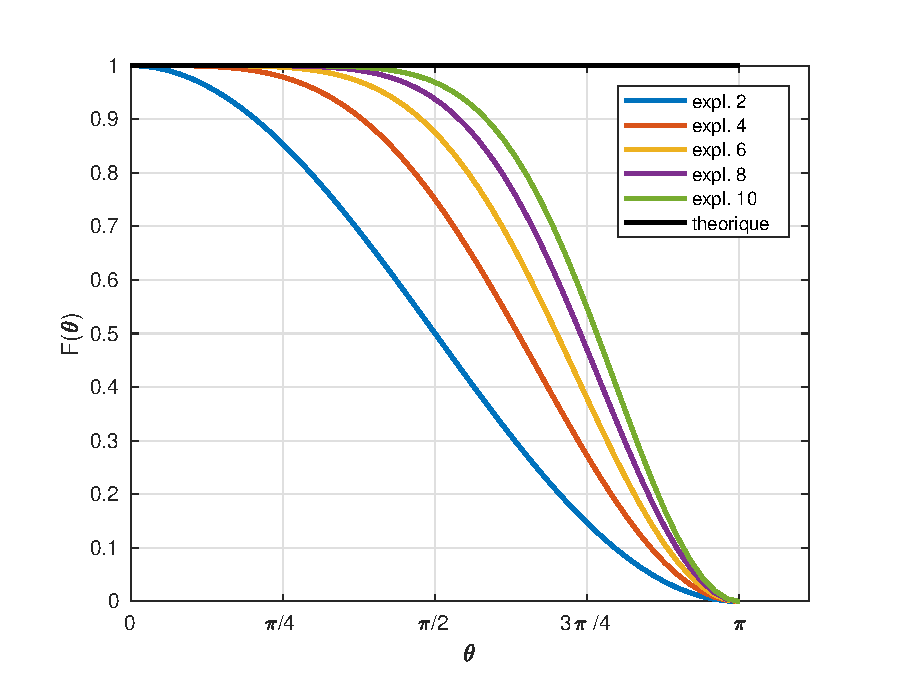
\includegraphics[scale=0.7]{freq_filter.eps}
\end{center}
\caption{Fonction d'amplification $\theta \mapsto S(e^{i\theta)})$ pour les filtres explicites d'ordre 2, 4, 6, 8 et 10.}
\label{fig:freq_filter}
\end{figure}
Pour plus de clareté, on représente dans le tableau \ref{tab:filter_095}, on représente la fréquence $\theta_{0.95}$ telle que
\begin{equation}
\begin{array}{rcl}
\beta(\theta) > 0.95 & \text{ si } & 0 \leq \theta \leq \theta_{0.95} \\
\beta(\theta) < 0.95 & \text{ si } & \theta_{0.95} \leq \theta \leq \pi.
\end{array}
\end{equation}

\begin{table}
\begin{center}
\begin{tabular}{|c||c|}
\hline
\textbf{Ordre du filtre : }$\mathbf{2J}$ & $\mathbf{\theta_{0.95}(J)}$\\
\hline
\hline
$10$&$1.6695$\\
$8$&$1.5165$\\
$6$&$1.3045$\\
$4$&$0.9851$\\
$2$&$0.4510$\\
\hline
\end{tabular}
\end{center}
\caption{Valeur de $\theta_{0.95}(J)$ pour quelques valeurs de $J$.}
\label{tab:filter_095}
\end{table}

Comme la fonction $\theta \mapsto \beta(\theta)$ est strictement décroissante et continue sur $[0,\pi]$, c'est une bijection de $[0,\pi]$ dans $[0,1]$ et on a 
\begin{equation}
\theta_{0.95}(J) = \arccos \left[ 1-2 (0.05)^{1/J} \right].
\end{equation}


La fonction $J \mapsto \theta_{0.95}(J)$ est strictement croissante donc lorsque $J$ croît, $\theta_{0.95}(J)$ croît et les fonctions sont moins affectées par le filtre $\mathcal{F}_{2J,x}$. De plus, 
\begin{equation}
\lim_{J \rightarrow +\infty} \theta_{0.95}(J) = \pi.
\end{equation}
Cependant, il faut noter que plus $J$ augmente, plus les fonctions manipulées sont supposées régulières donc ce qui précède n'est vrai que pour des fonctions de grilles très régulières.

\begin{remarque}
Le filtre $\mathcal{F}_{2J,x}$ est linéaire et agit sur les composantes des fonctions de grilles. Il existe $M_{2J} \in \mathbb{M}_N \left( \mathbb{R} \right)$ la matrice associée au filtrage des données en dimension 1 telle que
\begin{equation}
\mathcal{F}_{2J,x} \cdot \vec(\mathfrak{u}) = M_{2J} \vec(\mathfrak{u})
\end{equation}
La matrice $M_{2J}$ est donnée par
\begin{equation}
M_{2J} = S_{2J}(T),
\label{eq:matrice_filtrage}
\end{equation}
de plus, cette matrice est symétrique.
\end{remarque}































\section{Opérateurs aux différences en dimension 2}

Comme nous le verrons dans le chapitre \ref{chap:3}, la Cubed-Sphere est divisée en panel assimilables à des carrés en dimension 2. Pour cette raison, il est utile de considérer les opérateurs aux différences en dimension 2. Tous les opérateurs introduits dans la section précédente en dimension 1 peuvent être étendus à un carré périodique.


\subsection{Notations}
\label{sec:notation_2D}

En dimension 2, les notations sont analogues à celles utilisées en dimension 1. Si $a$ et $b$ sont des réels positifs, nous notons $\Omega = [a,b]^2$. Chaque côté du carré est de longueur $L=b-a$. Soient $u$ et $v$ dans $L^2(\Omega, \mathbb{C})$. Le produit scalaire est
\begin{equation}
(u,v) = \gint_{\Omega} u(x,y) \bar{v}(x,y) dx dy.
\end{equation}
La norme associée est :
\begin{equation}
\| u \|_{L^2(\Omega)} = \sqrt{(u,u)}. 
\end{equation}
On note également
\begin{equation}
\| u \|_{L^{\infty} ( \Omega )} = \max_{(x,y) \in \Omega} |u(x,y)|.
\end{equation}
Ces deux normes sont notées $\| u \|_{L^2}$ et $\| u \|_{L^{\infty}}$.

Dans le domaine $\Omega$, la grille est constituée des points $(x_i,y_j)_{0 \leq i,j \leq N}$ où $N \geq 1$ avec $a = x_0 < x_1 < \ldots < x_N = b$ et $a = y_0 < y_1 < \ldots < y_N = b$. Le pas d'espace $h$ est fixe et donné par $h = \frac{L}{N}$. Les points de grilles sont $(x_i, y_j)$ avec 
\begin{equation}
\left\lbrace\begin{array}{rcl}
x_i & = & a + i h \\
y_j & = & a + j h 
\end{array}\right. \text{ avec } 0 \leq i,j \leq N.
\end{equation}

Les points $(x_i,y_j)_{0 \leq i,j \leq N}$ sont de deux types (voir figure \ref{fig:maillage2D}) :
\begin{itemize}
\item Les points de bords $(x_i, y_j)$ avec
\begin{equation}
i \in \left\lbrace 0 , N \right\rbrace \text{ ou } j \in \left\lbrace 0 , N \right\rbrace,
\end{equation}
\item les points intérieurs $(x_i, y_j)$ avec
\begin{equation}
1 \leq i,j \leq N-1.
\end{equation}
\end{itemize}



\begin{figure}[htbp]
\begin{center}
\begin{tikzpicture}[scale=1.5]
	\draw (-3,-3.2) node[below] {$x_0=a$} ;
	\draw (-2,-3.2) node[below] {$x_1$} ;
	\draw (-1,-3.2) node[below] {$x_2$} ;
	\draw (0,-3.2) node[below] {$\ldots$} ;
	\draw (1,-3.2) node[below] {$x_{N-2}$} ;
	\draw (2,-3.2) node[below] {$x_{N-1}$} ;
	\draw (3,-3.2) node[below] {$x_N =b$} ;
	
	\draw (-3.2,-3) node[left] {$y_0=a$} ;
	\draw (-3.2,-2) node[left] {$y_1$} ;
	\draw (-3.2,-1) node[left] {$y_2$} ;
	\draw (-3.2,0) node[left] {$\vdots$} ;
	\draw (-3.2,1) node[left] {$y_{N-2}$} ;
	\draw (-3.2,2) node[left] {$y_{N-1}$} ;
	\draw (-3.2,3) node[left] {$y_N =b$} ;
	
	\draw (-3,-3) grid[step=1] (3,3);

	\draw (-3,-3) node[color=yellow] {$\bullet$} ;
	\draw (-3,-3) node {$\circ$} ;
	
	\foreach \k in {-3,...,3}
		{\draw  (\k,-3) node[color=white] {$\bullet$} ;
	   	\draw (\k,-3) node {$\circ$} ;
	   	\draw  (\k,3) node[color=white] {$\bullet$} ;
	   	\draw (\k,3) node {$\circ$} ;
	   	\draw  (-3,\k) node[color=white] {$\bullet$} ;
	   	\draw (-3,\k) node {$\circ$} ;
	   	\draw  (3,\k) node[color=white] {$\bullet$} ;
	   	\draw (3,\k) node {$\circ$} ;
	   	}
	   	
	\foreach \k in {-2,...,2}
		{\draw  (\k,-2) node {$\bullet$};
		\draw  (\k,-1) node {$\bullet$};
		\draw  (\k,0) node {$\bullet$};
		\draw  (\k,1) node {$\bullet$};
		\draw  (\k,2) node {$\bullet$};
	   	}
\end{tikzpicture}
\end{center}
\caption{Grille en dimension 2. Les symboles $\circ$ désignent les points de bords, les symboles $\bullet$ désignent les points intérieurs de la grille.}
\label{fig:maillage2D}
\end{figure}


Une fonction $u : (x,y) \in \mathbb{R} \mapsto u(x,y) \in \mathbb{C}$ est $L-$\textit{périodique} dans les directions $x$ et $y$ si 
\begin{equation}
\begin{array}{rcl}
u(x,y+L) & = & u(x,y) \\
u(x+L,y) & = & u(x,y)
\end{array} \text{ pour tous } (x,y) \in \mathbb{R}^2.
\end{equation}

Les notions de fonctions de grilles sont analogues à celles vues en dimension 1 :
\begin{enumerate}
\item Une \textit{fonction de grille} est une fonction définie aux points de la grille $(x_i,y_j)_{0 \leq i,j \leq N}$. Nous notons les fonctions en fonte gothique comme $\mathfrak{u}$ ou $\mathfrak{v}$. On note :
\begin{equation}
\mathfrak{u}_{i,j} = \mathfrak{u}(x_i,y_j) \text{ et }  \mathfrak{u} = \left( \mathfrak{u}_{i,j} \right)_{0 \leq i,j \leq N}.
\end{equation}
On note $L^2_h$ l'espace des fonctions de grilles. Cet espace est équipé d'un produit scalaire et de la norme associée :
\begin{equation}
(\mathfrak{u}, \mathfrak{v})_h = h^2 \gsum_{i,j=0}^N \mathfrak{u}(x_i, y_j) \bar{\mathfrak{v}}(x_i, y_j) \text{ et } |\mathfrak{u}|_h = \sqrt{(\mathfrak{u},\mathfrak{u})_h}.
\end{equation}
De plus, pour $\mathfrak{u}$ fonction de grille, on note
\begin{equation}
| \mathfrak{u} |_{\infty} = \max_{0 \leq i,j \leq N} |\mathfrak{u}_{i,j}|.
\end{equation}


\item Soit $u : (x,y) \in \Omega \mapsto u(x,y) \in \mathbb{R}$, nous définissons la fonction associée, notée $u^*$ est définie comme la restriction de $u$ à la grille :
\begin{equation}
u^*_{i,j} = u(x_i, y_j) \text{ pour tous } 0 \leq i,j \leq N.
\end{equation}

\item Cas périodique : $\mathfrak{u}$ est périodique si $\mathfrak{u}_{i,0} = \mathfrak{u}_{i,N}$ et $\mathfrak{u}_{0,j} = \mathfrak{u}_{N,j}$ pour tous $0 \leq i,j \leq N$. On note $L_{h,\per}^2$ l'espace des fonctions de grilles périodiques. Cet espace est doté du produit scalaire et de la norme
\begin{equation}
(\mathfrak{u},\mathfrak{v})_{h,\per} = h^2 \sum_{i,j=0}^{N-1} \mathfrak{u}_{i,j} \bar{\mathfrak{v}}_{i,j} \text{ et } |\mathfrak{u}|_{h,\per} = \sqrt{(\mathfrak{u}, \mathfrak{u})_{h,\per}}.
\end{equation}
Pour $u$ périodique selon $x$ et $y$, on a $u^*_{i,0}=u^*_{i,N}$ et $u^*_{0,j}=u^*_{N,j}$ pour tous $0 \leq i,j \leq N$.

\item Une fonction de grille $\mathfrak{u} \in L^2_h$est associée au vecteur $U \in \mathbb{R}^{(N+1)^2}$ dont les composantes sont les valeurs de $\mathfrak{u}$ dans l'ordre anti-lexicographique :
\begin{equation}
U = \begin{bmatrix}
\mathfrak{u}_{0,0}\\
\mathfrak{u}_{1,0}\\
\vdots \\
\mathfrak{u}_{N,0}\\
\mathfrak{u}_{0,1}\\
\mathfrak{u}_{1,1}\\
\vdots \\
\mathfrak{u}_{N,1}\\
\vdots \\
\mathfrak{u}_{N,N}\\
\end{bmatrix}.
\end{equation}
On note ces vecteurs par des lettres capitales.
\end{enumerate}















%
\subsection{Opérateurs aux différences en géométrie cartésienne}

On considère dans cette section les fonctions de grille périodiques $u \in L^2_{h,\per}$. Nous définissons les opérateur agissant sur les fonctions de grilles comme suit.

\begin{definition}
Les opérateurs $\tau_x$ et $\tau_y$ dans les directions $x$ et $y$ sont définis par
\begin{equation}
\left\lbrace
\begin{array}{rcl}
\tau_x \mathfrak{u}_{i,j} & = & \mathfrak{u}_{i+1,j}\\
\tau_y \mathfrak{u}_{i,j} & = & \mathfrak{u}_{i,j+1}\\
\end{array}
\right.
\end{equation}
avec $\mathfrak{u}$ une fonction de grille et $1 \leq i,j \leq N$. Il s'agit d'\textit{opérateurs de translations} dans les directions $x$ et $y$.
\end{definition}

Les opérateurs obtenus en dimension 1 sont définis en dimension 2 grâce à ces deux opérateurs de translation. Les opérateurs centrés dans les directions $x$ et $y$ par 
\begin{equation}
\left\lbrace
\begin{array}{rcl}
\delta_{2J,x} & = & \dfrac{1}{h} Q_{2J}(\tau_x) \\
\delta_{2J,y} & = & \dfrac{1}{h} Q_{2J}(\tau_y)
\end{array}
\right.
\label{eq:der_centrée_2D}
\end{equation}
De même, on définit les opérateurs dans chaque direction par 
\begin{equation}
\left\lbrace
\begin{array}{rcl}
\sigma_x & = & R(\tau_x) \\
\sigma_y & = & R(\tau_y) \\
\end{array}
\right.
\label{eq:simpson_2D}
\end{equation}
où $R$ est donné par $R(X) = (1-2 \beta) + \beta (X+X^{N-1})$.
Chacun des opérateurs $\sigma_x$ et $\sigma_y$ est inversible si $|\beta|<1/4$.
L'opérateur hermitien en dimension 1 $\delta_x^H$ est étendue en dimension 2 grâce à la relation suivante 
\begin{equation}
\left\lbrace
\begin{array}{rcl}
\delta_{2J+2,x}^H & = & \sigma_x^{-1} \circ \delta_{2J,x} \\
\delta_{2J+2,y}^H & = & \sigma_y^{-1} \circ \delta_{2J,y}
\end{array}
\right.
\label{eq:der_herm_2D}
\end{equation}

\begin{theoreme}
Soit $u : x \in \Omega \mapsto u(x) \in \mathbb{R}$ est une fonction de $\mathcal{C}^5 (\Omega)$. On note $u^*$ la fonction de grille associée à $u$. Alors
\begin{equation}
\begin{array}{rcl}
\|(\partial_x u)^* - \delta_{2P+2,x}^H u^*\|_{\infty} & \leq & C_x h^{2J+2} \| \partial_x^{(2J+3)}u \|_{\infty}\\
\|(\partial_y u)^* - \delta_{2P+2,y}^H u^*\|_{\infty} &\leq & C_y h^{2J+2} \| \partial_y^{(2J+3)}u \|_{\infty}
\end{array}
\end{equation}
où $C_x$, $C_y$ sont des réels positifs indépendants de $h$ et de $u$.
\end{theoreme}

\begin{proof}
Conséquence du théorème \ref{th:consistence_herm2} appliqué à chaque direction $x$ et $y$.
\end{proof}

























\subsection{Écriture matricielle des opérateurs aux différences en dimension 2}

Dans cette section, nous précisons les notations vectorielles et matricielles utiles en dimension 2.
La \textit{base canonique} de $\mathbb{R}^N$, notée $\left(e_i \right)_{0 \leq i \leq N-1}$ est donnée par 
\begin{equation}
\left( e_i \right) = \delta_{i,j} = \left\lbrace
\begin{array}{rl}
1 & \text{ si } j=i,\\
0 & \text{ sinon.}
\end{array}
\right.
\end{equation}
$\delta_{i,j}$ est le symbole de Kronecker.

\begin{definition}
Soit $A$ une matrice $m \times n$ et $B$ une matrice $p \times q$, avec $m, n, p, q \in \mathbb{N}^{\star}$. Le produit de Kronecker $A \otimes B$ est la matrice $mp \times nq$ définie par
\begin{equation}
A \otimes B = 
\begin{bmatrix}
a_{1,1}B & \cdots & a_{1,n}B \\ 
\vdots & \ddots & \vdots \\ 
a_{n,1}B & \cdots & a_{n,n}B
\end{bmatrix} .
\end{equation}
\end{definition}
Le produit de Kronecker possède les propriétés suivantes \cite{VanLoan1992} :

\begin{proposition}
Soient $A$, $B$, $C$ et $D$ des matrices complexes.
\begin{itemize}
\item Pour tout $\alpha \in \mathbb{C}$, on a
\begin{equation}
\alpha ( A \otimes B ) = (\alpha A) \otimes B = A \otimes (\alpha B),
\end{equation}

\item si $AC$ et $BD$ sont bien définis alors
\begin{equation}
(A \otimes B ) (C \otimes D) = AC \otimes BD,
\end{equation} 

\item par transposition, on a
\begin{equation}
(A \otimes B)^{T} = A^{T} \otimes B^{T}.
\end{equation}

\item si $A \in \mathbb{M}_n (\mathbb{C})$ et $B \in \mathbb{M}_p (\mathbb{C})$ sont inversibles, alors $A \otimes B$ est inversible et
\begin{equation}
(A \otimes B)^{-1} = A^{-1} \otimes B^{-1}.
\end{equation}

\item si $A \in \mathbb{M}_n (\mathbb{C})$ et $B \in \mathbb{M}_p (\mathbb{C})$ alors
\begin{equation}
\det (A \otimes B) = \det(A)^n \det(B)^p.
\end{equation}
\end{itemize}
\label{prop:pdt_kron}
\end{proposition}

\begin{proposition}
Soit $A \in \mathbb{M}_n(\mathbb{C})$ et $p \in \mathbb{N}^*$, alors les spectres des matrices $(A \otimes \I_p)$ et $(\I_p \otimes A)$ sont connus et on a
\begin{itemize}
\item $A \otimes \I_p \in \mathbb{M}_{np}(\mathbb{C})$ et
\begin{equation}
\Sp(A \otimes \I_p) = \Sp(A),
\end{equation}

\item $\I_p \otimes A \in \mathbb{M}_{np}(\mathbb{C})$ et
\begin{equation}
\Sp(\I_p \otimes A) = \Sp(A),
\end{equation}
\end{itemize}
où $\I_p$ désigne la matrice identité de $\mathbb{M}_p(\mathbb{C})$.
\label{prop:eigen_pdtkron}
\end{proposition}

\begin{proof}
\begin{itemize}
Soit $\lambda \in \Sp(A \otimes \I_p)$ alors $\lambda$ est solution de 
\begin{equation}
\det(A \otimes \I_p - \lambda \I_{np}) = 0
\end{equation}
Donc d'après la proposition \ref{prop:pdt_kron} et comme $\I_n \otimes \I_p = \I_{np}$, on a
\begin{align*}
\det((A \otimes \I_p)-\lambda \I_{np}) & = \det(A \otimes \I_p - \lambda \I_n \otimes \I_p) \\
	& = \det(A - \lambda \I_n)^p \det(\I_p \otimes \I_n)^n \\
	& = \det(A - \lambda \I_n)^p
\end{align*}
Ainsi, on a 
\begin{equation*}
\lambda \in \Sp(A\otimes \I_p) \Leftrightarrow \lambda \in \Sp(A).
\end{equation*}	
De là, il découle l'égalité souhaitée sur les ensembles :
\begin{equation}
\Sp(A \otimes \I_p) = \Sp(A).
\end{equation}
La seconde égalité est obtenue de la même manière.
\end{itemize}
\end{proof}

On note $\text{vec}_2$ l'opérateur suivant :

\begin{definition}
L'opérateur $\vec_2$ est défini par
\begin{equation}
\begin{array}{rcl}
\vec_2 : L^2_h & \longrightarrow & \mathbb{C}^{N^2}\\
\mathfrak{v} & \longrightarrow & V = \text{vec}_2(\mathfrak{v})
\end{array}
\end{equation}
avec
\begin{equation}
\text{vec}_2(\mathfrak{v}) = \gsum_{i,j=0}^{N-1} \left( e_j \otimes e_i \right)\mathfrak{v}_{i,j}.
\end{equation}
\end{definition}

L'opérateur $\vec_2$ applique une fonction de grille $\mathfrak{v} \in L^2_{h,\per}$ en un vecteur $V \in \mathbb{C}^{N^2}$ dont les composantes sont déduites de $\mathfrak{v}$ dans l'ordre antilexicographique. Autrement dit $V = \vec_2(\mathfrak{v})$ est donné par
\begin{equation}
V=[\mathfrak{v}_{0,0}, \mathfrak{v}_{1,0}, \mathfrak{v}_{2,0}, \cdots, \mathfrak{v}_{N-1,0}, \mathfrak{v}_{0,1}, \mathfrak{v}_{1,1}, \cdots,  \mathfrak{v}_{N-1,1}, \mathfrak{v}_{N-1,N-1}]^T.
\end{equation}
On note $\vec$ au lieu de $\vec_2$ quand le contexte est clair.


\begin{proposition}
Soit $\mathfrak{u}$ une fonction de grille. Alors les opérateurs de dérivées centrées \eqref{eq:der_centrée_2D} s'écrivent matriciellement sous la forme
\begin{equation}
\left\lbrace
\begin{array}{rcl}
\text{vec}(\delta_{2J,x} \mathfrak{u}) & = & (\I_N \otimes D_{2J}) \text{vec}(\mathfrak{u})\\
\text{vec}(\delta_{2J,y} \mathfrak{u}) & = & (D_{2J} \otimes \I_N) \text{vec}(\mathfrak{u})\\
\text{vec}(\sigma_x \mathfrak{u}) & = & (\I_N \otimes P_{\sigma}) \text{vec}(\mathfrak{u})\\
\text{vec}(\sigma_y \mathfrak{u}) & = & (P_{\sigma} \otimes \I_N) \text{vec}(\mathfrak{u})\\
\end{array}\right.
\end{equation}
où $D_{2J}$ est issu de \eqref{eq:matrice_explicite} et $P_{\sigma}$ de \eqref{eq:matrice_implicitpart}.
\label{prop:op_der_simpson_mat}
\end{proposition}

\begin{proof}
Par définition de $\text{vec}_2$, on a 
\begin{align*}
\text{vec} (\delta_{2J,x} \mathfrak{u}) & = \gsum_{i,j=0}^J (e_j \otimes e_i) \delta_{2J,x} \mathfrak{u}_{i,j} \\
	& = \gsum_{i,j=0}^{N-1} \gsum_{p=1}^J (e_j \otimes e_i) \dfrac{a_p}{2ph} (\mathfrak{u}_{i+p,j} - \mathfrak{u}_{i-p,j}) \\
	& = \gsum_{p=1}^J \dfrac{a_p}{2ph} \left( \gsum_{i,j=0}^{N-1} (e_j \otimes e_i) \mathfrak{u}_{i+p,j} - (e_j \otimes e_i) \mathfrak{u}_{i-p,j} \right) \\
	& = \gsum_{p=1}^J \dfrac{a_p}{2ph} \gsum_{i,j=0}^{N-1} e_j \otimes (e_i \mathfrak{u}_{i+p,j} - e_i\mathfrak{u}_{i-p,j})\\
	& = \gsum_{p=1}^J \dfrac{a_p}{2ph} \left( \I_N \otimes \left( T^p - T^{-p}  \right) \right) \vec (\mathfrak{u}) \\
	& = (\I_N \otimes D_{2J}) \vec (\mathfrak{u})
\end{align*}
les autres égalités se montrent de la même manière.
\end{proof}
On déduit également $\vec(\delta_{2J+2,x}^H \mathfrak{u})$ et $\vec(\delta_{2J+2,y}^H \mathfrak{u})$.
On considère à présent les matrices associées à $\delta^H_{2J+2,x} \mathfrak{u}$ et $\delta^H_{2J+2,y} \mathfrak{u}$.
\begin{theoreme}
Soit $\mathfrak{u}$ une fonction de grille. Alors, si on pose 
\begin{equation}
\left\lbrace
\begin{array}{rcl}
U & = & \text{vec} (\mathfrak{u}) \\
U_x & = & \text{vec} (\delta_{2J+2,x}^H \mathfrak{u}) \\
U_y & = & \text{vec} (\delta_{2J+2,y}^H \mathfrak{u}) \\
\end{array}
\right.
\end{equation}
les matrices associées à $\delta^H_{2J+2,x} \mathfrak{u}$ et $\delta^H_{2J+2,y} \mathfrak{u}$ sont telles que 
\begin{equation}
\left\lbrace
\begin{array}{rcccl}
U_x &=& (\I_N \otimes P^{-1}_{\sigma} D_{2J})U \\
U_y &=& (P^{-1}_{\sigma}D_{2J} \otimes \I_N)U.
\end{array}
\right.
\end{equation}
\end{theoreme}

\begin{proof}
L'égalité suivante sont vérifiée
\begin{equation}
(P_{\sigma} \otimes I_N) U_x = (D_{2J} \otimes \I_N) U.
\end{equation}
Donc on obtient
\begin{align*}
U_y & = (P_{\sigma} \otimes I_N)^{-1}(D_{2J} \otimes \I_N) U \\
	& = (P^{-1}_{\sigma} D_{2J} \otimes \I_N^{-1}\I_N) U \\
	& = (P^{-1}_{\sigma} D_{2J} \otimes \I_N) U.
\end{align*}
La seconde égalité est obtenue de la meme manière.
\end{proof}

Les matrices $(Id \otimes P^{-1}D_{2P})$ et $(P^{-1}D_{2P} \otimes Id)$ sont antisymétrique.

\begin{proposition}
Les valeurs propres de $\delta_{2J+2,x}$ et de $\delta_{2J+2,y}$ sont
\begin{equation}
\dfrac{1}{h}Q^H_{2J+2}(\omega^k)
\end{equation}
pour $-N/2+1 \leq k \leq N/2$.
\end{proposition}

\begin{proof}
Il s'agit d'une conséquence de la proposition \ref{prop:eigen_pdtkron}.
\end{proof}











\subsection{Opérateur de filtrage}

Dans cette partie, nous utilisons les notations de la section \ref{sec:notation_2D} en contexte périodique. Définissons les opérateurs de filtrage bidimensionnel dans les directions $x$ et $y$ par
\begin{equation}
\left\lbrace
\begin{array}{rcl}
\mathcal{F}_{2J,x} & = & \gsum_{p=0}^J a_p \dfrac{\tau_x^p + \tau_x^{-p}}{2}  = S_{2J}(\tau_x), \\
\mathcal{F}_{2J,y} & = & \gsum_{p=0}^J a_p \dfrac{\tau_y^p + \tau_y^{-p}}{2} = S_{2J}(\tau_y).
\end{array}
\right.
\end{equation}
où $S_{2J}$ est donné par \eqref{eq:pol_filtrage}. 
Les coefficients $(a_p)_{0 \leq p \leq J}$ vérifient le système \eqref{eq:system_ftr}. Les opérateurs $\mathcal{F}_{2J,x}$ et $\mathcal{F}_{2J,y}$ commutent :
\begin{equation}
\mathcal{F}_{2J,x} \circ \mathcal{F}_{2J,y} = \mathcal{F}_{2J,y} \circ \mathcal{F}{2F,x}.
\end{equation}
La proposition \ref{prop:filter_def} permet de vérifier la consistance des opérateurs de filtrages.
Si $u : (x,y) \in \Omega \mapsto u(x,y) \in \mathbb{R}$ est fonction de $\mathcal{C}^{2F}$ alors :
\begin{equation}
\left\lbrace
\begin{array}{rcl}
\| u^* - \mathcal{F}_{2J,x}u^* \|_{\infty} & \leq & C_x h^{2J} \| \partial_x^{(2J)}u \|_{\infty}\\
\| u^* - \mathcal{F}_{2J,y}u^* \|_{\infty} & \leq & C_y h^{2J} \| \partial_y^{(2J)}u \|_{\infty}
\end{array}
\right.
\end{equation}
où $C_x$ et $C_y$ sont des constantes indépendantes de $u$ et de $h$.
En composant les opérateurs, l'opérateur $\mathcal{F}_{2J,x} \circ \mathcal{F}_{2J,y}$ désigne un opérateur de Filtrage au sens où
\begin{equation}
\| u^* - (\mathcal{F}_{2J,x} \circ \mathcal{F}_{2J,y}) u^* \|_{\infty} = C h^{2J} \max (\| \partial_x^{(2J)}u \|_{\infty}, \| \partial_y^{(2J)}u \|_{\infty}).
\end{equation}
où $C$ est un réel indépendant de $u$ et de $h$.

L'écriture matricielle de l'opérateur de filtrage est donnée par la proposition suivante :
\begin{proposition}
Soit $\mathfrak{u} \in L^2_{h,\per}$ une fonction de grille. Alors les opérateurs de filtrages
\begin{equation}
\left\lbrace
\begin{array}{rcl}
\text{vec} (\mathcal{F}_{2J,x} \mathbf{u}) & = & (\I_N \otimes M_{2J}) \text{vec} (\mathbf{u})\\
\text{vec} (\mathcal{F}_{2J,y} \mathbf{u}) & = & (M_{2J} \otimes \I_N) \text{vec} (\mathbf{u})\\
\end{array}
\right.
\end{equation}
\end{proposition}
Comme la matrice $M_{2J}$ est symétrique, il est immédiat que $\I_N \otimes M_{2J}$ et $M_{2J} \otimes \I_N$ sont symétriques.
% disc.tex
\chapter{Analyse numérique}

\section{Opérateur de filtrage }

\subsection{Opérateur de filtrage en dimension 1}

Lors de la discrétisation via un schéma aux différences finies et suite à la discrétisation en temps, des oscillations parasites du type "+1/-1" peuvent apparaître. Il s'agit de phénomènes haute fréquences qui peuvent provoquer des instabilités numériques. 

Si $\mathfrak{u}$ est une fonction de grille périodique, on note le filtre passe-bas $\mathcal{F}\mathfrak{u}$. Dans la pratique, nous cherchons $\mathcal{F}$ sous la forme 

\begin{equation}
\mathcal{F} = \gsum_{k=0}^F a_k \dfrac{\tau^k + \tau^{-k}}{2}
\label{eq:ftr}
\end{equation}

Les coefficients $(a_k)_{0 \leq k \leq F}$ sont déterminés de manière à supprimer les phénomènes oscillants hautes fréquences (figure \ref{fig:hf_waves}) de la formes $\mathfrak{u}$ avec 
\begin{equation}
\mathfrak{u}_j = (-1)^j
\end{equation}

\begin{figure}[htbp]
\begin{center}
\begin{tikzpicture}[scale=1.4]
	\draw (-4,1) -- (-3,-1) ;
	\draw (-3,-1) -- (-2,1) ;
	\draw (-2,1) -- (-1,-1) ;
	\draw (-1,-1) -- (0,1) ;
	\draw (0,1) -- (1,-1) ;
	\draw (1,-1) -- (2,1) ;
	\draw (2,1) -- (3,-1) ;
	\draw (3,-1) -- (4,1) ;
	
	\draw (4,0) -- (-4,0) ;
	\foreach \k in {-3,...,3}
		{\draw  (\k,0) node[color=blue] {$\bullet$} ;
	   	\draw (\k,0) node {$\circ$} ;
	   	}
\end{tikzpicture}
\end{center}
\caption{Ondes de type "+1/-1".}
\label{fig:hf_waves}
\end{figure}


En considérant cette fonction de grille, on cherche $(a_k)_{0\leq k \leq F}$ tels que $\mathcal{F} \mathfrak{u} = \mathfrak{0}$, soit :
\begin{equation}
\mathcal{F}\mathfrak{u}_i = \gsum_{k=0}^F a_k \dfrac{\mathfrak{u}_{i+k} + \mathfrak{u}_{i-k}}{2} = \gsum_{k=0}^F a_k  \dfrac{(-1)^{i+k} + (-1)^{i-k}}{2} = 0.
\end{equation}
Cette équation est équivalente à 
\begin{equation}
\gsum_{k=0}^F a_k (-1)^k = 0
\label{eq:ftr_ftrcond}
\end{equation}
La relation \eqref{eq:ftr_ftrcond} nous donne une condition alors qu'il y a $F+1$ paramètres à déterminer. Il reste $F$ degrés de libertés dans l'opérateur de filtrage. Le choix qui est fait est de maximiser l'ordre du filtrage de manière à perturber un minimum la donnée initiale tout en supprimant les ondes parasites.

Le filtre doit conserver les très basses fréquences, lorsque $\mathfrak{u} = \mathfrak{1}$, on doit alors $\mathcal{F}\mathfrak{u} = \mathfrak{1}$.
C'est à dire que les coefficients $(a_k)_{0 \leq k \leq F}$ vérifient la relation de consistance
\begin{equation}
\gsum_{k=0}^F a_k = 1
\label{eq:ftr_conscond}
\end{equation}

Enfin, on remarque que si $u : x \in \Omega \mapsto u(x) \in \mathbb{R}$ et si $u^*$ est la fonction de grille associée à $u$, alors on a 
\begin{equation}
\begin{array}{rcl}
u(x_i + kh) & = & u(x_i) + p k u'(x_j) + \cdots + \dfrac{(kh)^l}{l!}u^{(l)}(x_i) + \cdots +\dfrac{(kh)^{2F}}{2F!} u^{(2F)}(\xi_k)\\
u(x_i - kh) & = & u(x_i) - p k u'(x_j) + \cdots + \dfrac{(-kh)^l}{l!}u^{(l)}(x_i) + \cdots +\dfrac{(-kh)^{2F}}{2F!} u^{(2F)}(\eta_k)
\end{array}
\end{equation}
avec $\xi_k \in [x_i, x_i+kh]$ et $\eta_k \in [x_i-kh, x_i]$. Alors par combinaison linéaire en considérant \eqref{eq:ftr_conscond} vérifiée, 
\begin{equation}
\mathcal{F}u^* - u^* = \gsum_{l=1}^{2F-1} \gsum_{k=0}^F \dfrac{a_k}{2} \underbrace{\dfrac{(kh)^l + (-kh)^l}{l!}}_{=0 \text{ pour } l \text{ impair.}}u^{(l)}(x_i) + \gsum_{k=0}^F \dfrac{a_k}{2}\dfrac{(kh)^{2F}}{2F!} \left( u^{(2F)}(\xi_k) + u^{(2F)}(\eta_k) \right)
\end{equation}
Ainsi, la condition de précision est 
\begin{equation}
\gsum_{k=0}^F a_k k^{2l} = 0 \text{ pour } 1 \leq l \leq F-1.
\label{eq:ftr_prescond}
\end{equation}

\begin{theoreme}
Soit $F \in \mathbb{N}^{\star}$. Il existe un unique $(a_k)_{0 \leq k \leq F}$ tel que $\mathcal{F}$ soit à la fois consistant en vérifiant \eqref{eq:ftr_conscond}, précis en vérifiant \eqref{eq:ftr_prescond} et soit un filtre passe bas en satisfesant \eqref{eq:ftr_ftrcond}. L'erreur de troncature du filtre est alors donnée par 
\begin{equation}
\mathcal{F}u^* - u^* = h^{2F} \gsum_{k=0}^F \dfrac{a_k}{2} \dfrac{k^{2F}}{2F!} \left( u^{(2F)}(\xi_k) + u^{(2F)}(\eta_k) \right).
\end{equation}
\label{prop:filter_def}
\end{theoreme}

\begin{proof}
La forme de l'erreur de troncature a déjà été vue, il reste à prouver l'unicité.

Après avoir retiré \eqref{eq:ftr_ftrcond} à \eqref{eq:ftr_conscond}, dire qu'il existe une unique $(a_j)_{0 \leq j \leq J}$ satisfesant les conditions est équivalent à dire que la matrice

\begin{equation}
A=\begin{bmatrix}
1 &  1  &  1  &  1  &  1  &  1  & \cdots\\  
0 &  2  &  0  &  2  &  0  & 2  & \cdots\\
0 &  1  & 2^2 & 3^2 & 4^2 & 5^2 & \cdots\\
0 &  1  & 2^4 & 3^4 & 4^4 & 5^4 & \cdots\\
0 &  1  & 2^6 & 3^6 & 4^6 & 5^6 & \cdots\\
&&& \vdots &  \vdots &
\end{bmatrix} \in \mathcal{M}_{J+1} \left( \mathbb{R} \right)
\end{equation}
est inversible car $a = [a_0, a_1, \cdots, a_J]^T$ est solution de 
\begin{equation}
A a = e_1
\end{equation}
avec $e = [1,1/2, 0,\cdots,0]^T$. En développant la seconde ligne de $A$, on a
\begin{equation}
\det ( A ) = \begin{vmatrix} 
2  &  0  &  2  &  0  & 2  & \cdots\\
1  & 2^2 & 3^2 & 4^2 & 5^2 & \cdots\\
1  & 2^4 & 3^4 & 4^4 & 5^4 & \cdots\\
1  & 2^6 & 3^6 & 4^6 & 5^6 & \cdots\\
& & \vdots &  \vdots &
\end{vmatrix} = 2 \sum_{k=1}^{\lfloor\frac{F-1}{2}\rfloor} \Delta_{2k+1}
\end{equation}
avec $\Delta_k$ donné par
\begin{equation}
\Delta_k = \begin{vmatrix} 
1 & 2^2 & \cdots & (k-1)^2 & (k+1)^2 & \cdots\\
1 & 2^4 & \cdots & (k-1)^4 & (k+1)^4 & \cdots\\
1 & 2^6 & \cdots & (k-1)^6 & (k+1)^6 & \cdots\\
&&& \vdots &  \vdots &
\end{vmatrix} = \dfrac{((F-1)!)^2}{k^2} \begin{vmatrix} 
1 & 1 & \cdots & 1 & 1 & \cdots\\
1 & (2^2)^1 & \cdots & ((k-1)^2)^1 & ((k+1)^2)^1 & \cdots\\
1 & (2^2)^2 & \cdots & ((k-1)^2)^2 & ((k+1)^2)^2 & \cdots\\
&&& \vdots &  \vdots &
\end{vmatrix}
\end{equation}
On reconnait alors un déterminant de Van-Der-Monde, donc $\Delta_k = \prod_{1 \leq i < j \leq F-1} \left( \alpha_j - \alpha_i \right)$, avec 
\begin{equation}
\alpha_j = \left\lbrace
\begin{array}{ll}
j^2 & \text{ avec } 1 \leq j \leq k-1\\
(j+1)^2 & \text{ avec } k \leq j \leq J-2\\
\end{array}
\right.
\end{equation}
Alors si $i<j$, on a $\alpha_i < \alpha_j$, donc $\Delta_k>0$ et même $\det A$ est une somme de déterminants tous strictements positifs donc $\det A > 0$. $A$ est inversible et le résultat est prouvé.
\end{proof}
Quelques filtres particuliers sont donnés dans la table \ref{tab:filter} en fonction de leur ordre de précision.

\begin{table}[htbp]
\begin{center}
\begin{tabular}{|c||cccccc|}
\hline
\textbf{Ordre de précision} & $a_0$ & $a_1$ & $a_2$ & $a_3$ & $a_4$ & $a_5$ \\
\hline \hline
$2$ & $1/2$ & $1/2$ & & & & \\
\hline
$4$ & $10/16$ & $8/16$ & $-2/16$ & & & \\
\hline
$6$ & $44/64$ & $30/64$ & $-12/64$ & $2/64$ & & \\
\hline
$8$ & $186/256$ & $112/256$ & $-56/256$ & $16/256$ & $-2/256$ & \\
\hline
$10$ & $772/1024$ & $420/1024$ & $-240/1024$ & $90/1024$ & $-20/1024$ & $2/1024$ \\
\hline
\end{tabular}
\end{center}
\caption{Exemples de filtres de la forme \eqref{eq:ftr} et leurs ordres de précision.}
\label{tab:filter}
\end{table}

Dans la suite, nous supposerons que $(a_k)_{0 \leq k \leq F}$ satisfait les conditions \eqref{eq:ftr_conscond}, \eqref{eq:ftr_prescond} et \eqref{eq:ftr_ftrcond}.
Les valeurs propres et fonctions propres de $\mathcal{F}$ sont issues de la proposition \ref{prop:eigen_P(tau)}. Le résultat est immédiat.

\begin{theoreme}
Les valeurs propres de $\mathcal{F}$ sont données par $\beta^k$ avec 
\begin{equation}
\beta^k = \gsum_{f=0}^F a_k \cos \left( \dfrac{2 \pi k f}{N} \right)
\end{equation}
pour tout $0 \leq k \leq N-1$, $\beta^k$ est associé à la fonction propre $\mathfrak{u}^k$ telle que 
\begin{equation}
\mathfrak{u}^k_j = \exp \left[ i j \dfrac{2 \pi k}{N} \right].
\end{equation}
\end{theoreme}

On définit le \textit{symbole} du filtre $\mathcal{F}$ par la fonction $\beta : \theta \in [0, \pi] \mapsto \beta(\theta) \in \mathbb{R}$ donnée par :
\begin{equation}
\beta( \theta ) = \gsum_{f=0}^F a_k \cos \left( f \theta \right)
\end{equation}

\begin{proposition}
Il existe un unique polynôme $P$ de degré $F$ tel que 
\begin{equation}
\beta(\theta) = P(\cos \theta )
\end{equation}
De plus,
\begin{equation}
P(x) = 1 -\dfrac{1}{(-2)^F} (X - 1)^F.
\end{equation}
\end{proposition}

\begin{proof}
Soit $\theta \in [0, \pi]$, 
\begin{equation}
\beta(\theta) = \gsum_{f=0}^F a_f \cos \left( f \theta \right) = \gsum_{f=0}^F a_f T_f ( \cos \theta )
\end{equation}
où $T_f \in \mathbb{R}_f [X]$ est le $k-$ieme polynome de Tchebytchev. 
Ainsi il existe $P \in \mathbb{R}_F [x]$ tel que $\beta( \theta ) = P( \cos \theta )$. Ce polynôme est unique. Montrons que 
\begin{equation}
P(x) = 1 -\dfrac{1}{(-2)^F} (X - 1)^F.
\end{equation}
convient.

\begin{itemize}
\item on montre facilement que 
\begin{equation}
P( \cos 0 ) = 1 -\dfrac{1}{(-2)^F} (\cos 0 - 1)^F = 1,
\end{equation}
de même,
\begin{equation}
P( \cos \pi ) = 1 -\dfrac{1}{(-2)^F} (\cos \pi - 1)^F 1 -\dfrac{(-2)^F}{(-2)^F} = 0.
\end{equation}
\item On rappelle la formule de Fàa Di Bruno permettant de calculer la dérivée $n-$ième d'une composée. Si $f$ et $g$ sont des fonctions régulières, on a 
\begin{equation}
\dfrac{d^n}{dx^n} \left( f \circ g \right)(x) = \gsum_{k=1}^n f^{(k)}\left( g(x) \right) B_{n,k}\left( g'(x), g''(x), \cdots , g^{n-k+1}(x) \right)
\end{equation}
où $B_{n,k}$ est un polynôme de Bell. En utilisant cette formule avec $f = P$ et $g = \cos$, évaluée en $\theta = 0$, on montre que :
\begin{equation}
\dfrac{d^n}{d\theta^n} \left( P \circ \cos \right)(0) = \gsum_{k=1}^n P^{(k)}\left(1\right) B_{n,k}\left( -1,0,1,0, \cdots\right)
\end{equation}
Or, $P^{(k)}\left(1\right) = 0$ pour tout $k \geq 1$. Donc 
\begin{equation}
\dfrac{d^n}{d\theta^n} \left( P \circ \cos \right)(0) = 0
\end{equation}
\end{itemize}
Le polynôme $P$ convient et 
\begin{equation}
\beta( \theta ) = 1 - \dfrac{1}{(-2)^F}(\cos \theta -1)^F.
\end{equation}
\end{proof}

\begin{proposition}
Pour tout $\theta \in [0, \pi]$, on a 
\begin{equation}
0 \leq \beta ( \theta ) \leq 1
\end{equation}
\end{proposition}

\begin{proof}
Supposons qu'il existe $\theta \in [0, \pi]$ tel que $\beta(\theta) < 0$ ou $\beta(\theta) > 1$. Comme $\beta(0)=1$ et $\beta(\pi) = 0$, il existe $\tilde{\theta} \in ]0, \pi[$ tel que 
\begin{equation}
\beta'(\tilde{\theta}) = - \sin \tilde{\theta} P'(\cos \tilde{\theta} ) = 0
\end{equation}
Or $\sin \tilde{\theta} \neq 0$ pour $\tilde{\theta} \in ]0, \pi[$.
De plus, 
\begin{equation}
P'(X) = \dfrac{F}{(-2)^F}(X-1)^{F-1}
\end{equation}
donc en prenant $X = \cos \tilde{\theta}$,
\begin{equation*}
P'(X) = 0 \Leftrightarrow \cos \tilde{\theta} = 1
\end{equation*}
Ce qui est impossible pour $\tilde{\theta} \in ]0, \pi[$. Donc par l'absurde, le résultat est vérifié.
\end{proof}

La fonction $\beta$ permet de considérer le comportement du filtre sur les différentes fréquences $\theta \in [0, \pi]$. Les basses fréquences sont bien conservées alors que les hautes fréquences ($\theta$ proche de $\pi$) sont atténuées. Cette observation est visible sur la figure \ref{fig:freq_filter} représentant la fonction $\beta : \theta \mapsto \beta(\theta)$ associée aux filtres d'ordre 2, 4, 6, 8 et 10. 

\begin{figure}[htbp]
\begin{center}
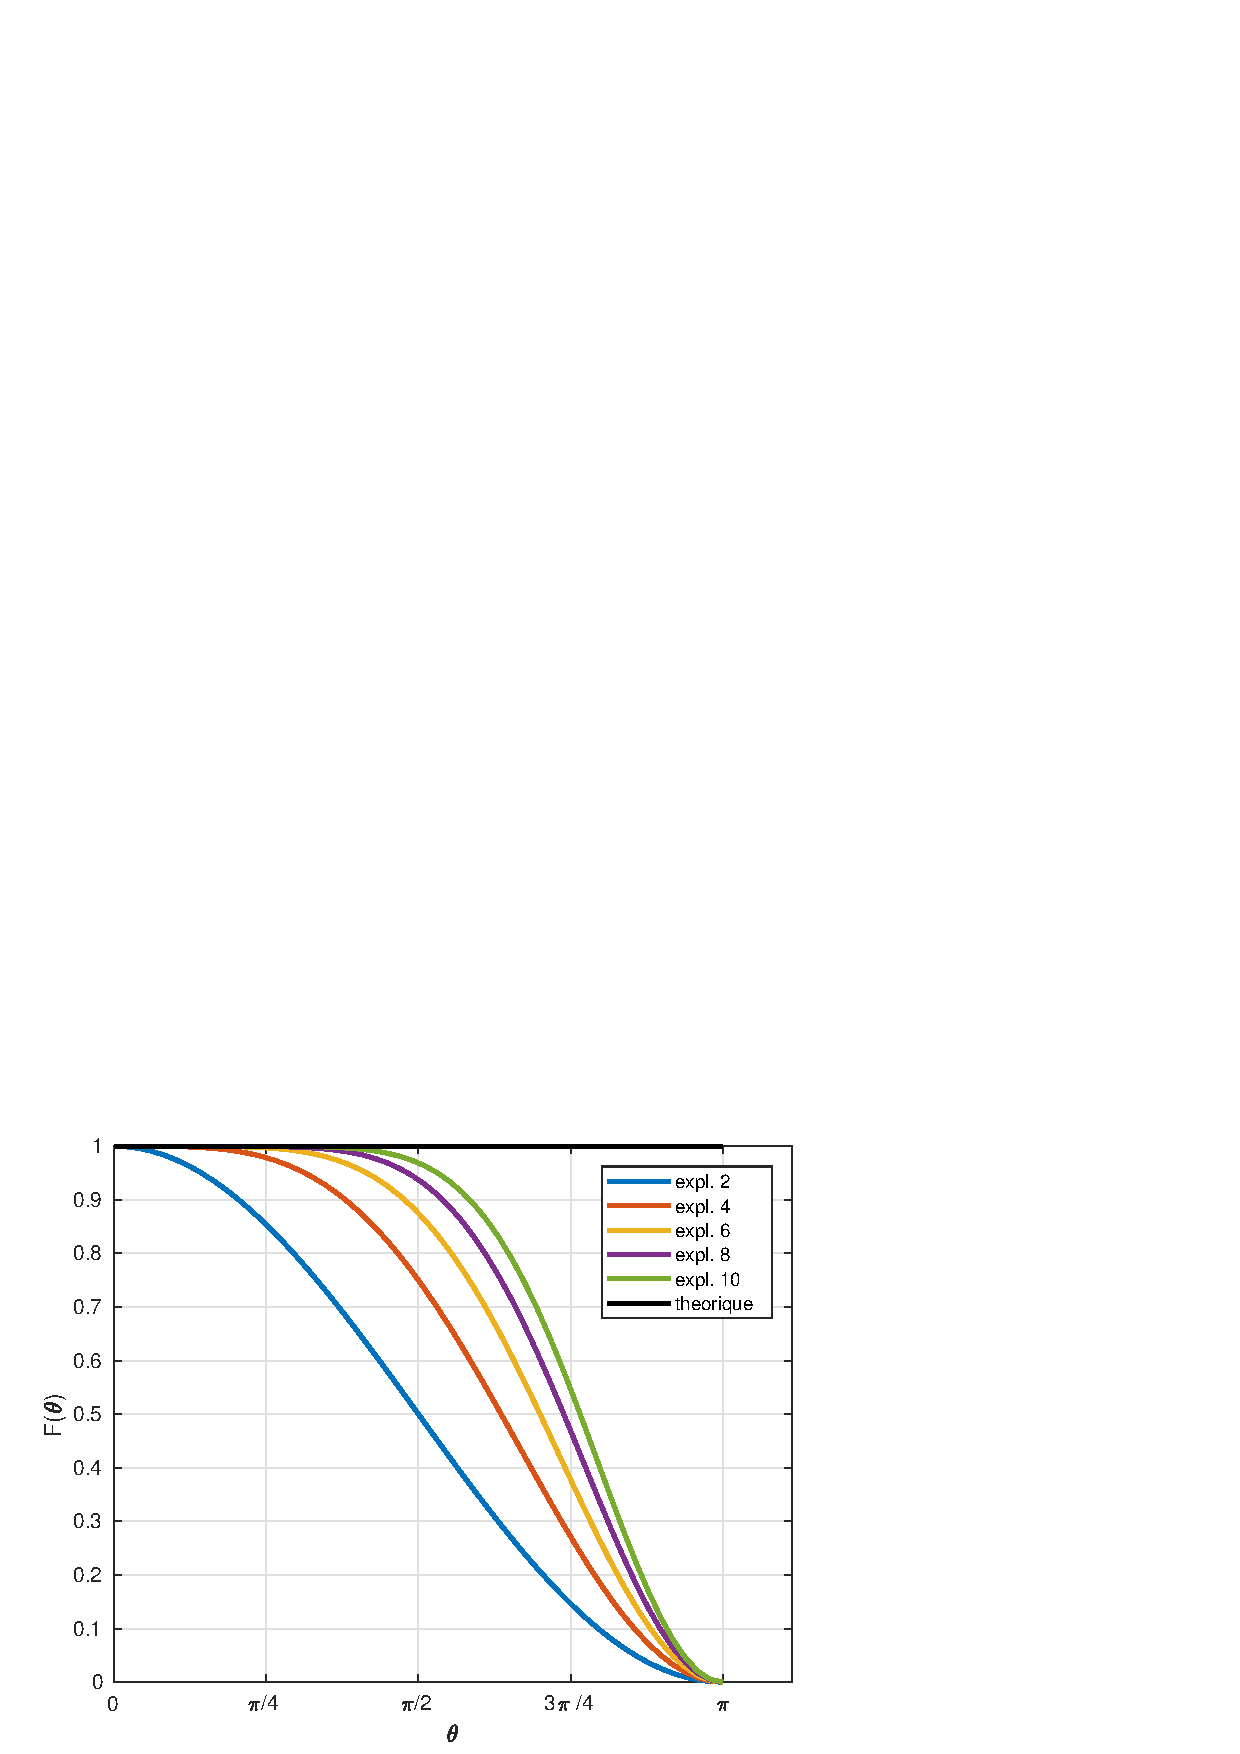
\includegraphics[scale=0.7]{freq_filter.png}
\end{center}
\caption{Fonction d'amplification $\beta$ pour les filtres explicites d'ordre 2, 4, 6, 8 et 10.}
\label{fig:freq_filter}
\end{figure}
Comme on s'y attendais, un filtre d'ordre élevé laisse passer un plus grand nombre de basses fréquences. Dans le tableau \ref{tab:filter_095}, on représente la fréquence $\theta_{0.95}$ maximale qui est conservée à $95\%$. Comme la fonction $\beta$ est strictement décroissante sur $[0,\pi]$, c'est une bijection de $[0,pi]$ dans $[0,1]$ et on a 
\begin{equation}
\theta_{0.95} = \beta^{-1}(0.95).
\end{equation}

\begin{table}
\begin{center}
\begin{tabular}{|c||c|}
\hline
\textbf{Ordre du filtre} & \textbf{Fréquence conservée à } $95\%$\\
\hline
\hline
$10$&$1.6695$\\
$8$&$1.5165$\\
$6$&$1.3045$\\
$4$&$0.9851$\\
$2$&$0.4510$\\
\hline
\end{tabular}
\end{center}
\caption{Fréquence conservée à $95\%$ en fonction de l'ordre du filtre.}
\label{tab:filter_095}
\end{table}

En pratique, cette fréquence $\theta_{0.95}$ est donnée en résolvant $\beta(\theta_{0.95})=0.95$ par 
\begin{equation}
\theta_{0.95} = \arccos \left[ 1-2 (0.05)^{1/F} \right].
\end{equation}
On remarque directement que la fonction $F \mapsto \theta_{0.95}$ est croissante, ce qui confirme que lorsque l'ordre de précision croit, $J$ croit et $\theta_{0.95}$ croit donc le filtre conserve un plus grand nombre de fréquences. De plus, 
\begin{equation}
\lim_{F \rightarrow \infty} \theta_{0.95} = \pi.
\end{equation}
Ce qui confirme la prise en compte d'un grand nombre de fréquence lorsque l'on augmente l'ordre du filtre. Cependant lorsque l'ordre du filtre augmente, l'effet de filtrage des hautes fréquences diminue.

Si $\mathfrak{u}$ est une fonction de grille, on pose $U$ et $\tilde{U}$ les vecteurs de $\mathbb{R}^N$ tel que
\begin{equation}
U = \begin{bmatrix}
\mathfrak{u}_1\\
\mathfrak{u}_2\\
\vdots \\
\mathfrak{u}_N\\
\end{bmatrix} \text{ et } 
\tilde{U} = \begin{bmatrix}
\mathcal{F}\mathfrak{u}_1\\
\mathcal{F}\mathfrak{u}_2\\
\vdots \\
\mathcal{F}\mathfrak{u}_N\\
\end{bmatrix}
\end{equation}
Alors $U$ et $\tilde{U}$ vérifient la relation
\begin{equation}
\tilde{U} = M F
\end{equation}
avec $M \in \mathcal{M}_N \left( \mathbb{R} \right)$ la matrice associée au filtrage des données en dimension 1 (dans le cas $F=2$):
\begin{equation}
M = \dfrac{1}{2}
\begin{bmatrix}
2a_0 & a_1 & a_2 &   &   &   & a_2 & a_1 \\ 
a_1 & 2 a_0 & a_1 & a_2 &   &   &   & a_2 \\ 
a_2 & a_1 & 2a_0 & a_1 & a_2 & (0) &   &   \\ 
  & a_2 & a_1 & 2a_0 & a_1 & a_2 &   &   \\ 
  &   & \ddots & \ddots & \ddots & \ddots & \ddots &   \\ 
  &   & (0) & a_2 & a_1 & 2 a_0 & a_1 & a_2 \\ 
a_2 &   &   &   & a_2 & a_1 & 2a_0 & a_1 \\ 
a_1 & a_2 &   &   &   & a_2 & a_1 & 2a_0
\end{bmatrix} 
\end{equation}
ou plus généralement 
\begin{equation}
M_{i,j} = \left\lbrace
\begin{array}{cl}
a_0 & \text{ si } i=j \\
\dfrac{1}{2} a_k & \text{ si } i+j \equiv k [N]\\
0 & \text{ sinon.}
\end{array}
\right.
\end{equation}
Il est clair que la matrice $M$ est symétrique.








\subsection{Opérateur de filtrage en géométrie cartésienne 2D}

Dans cette partie, nous utilisons toujours les notations de la section \ref{sec:notation_2D} en contexte périodique. Définissons les opérateurs de filtrage dans les directions $x$ et $y$ par
\begin{eqnarray*}
\mathcal{F}_x = \gsum_{k=0}^F a_k \dfrac{\tau_x^k + \tau_x^{-k}}{2} \\
\mathcal{F}_y = \gsum_{k=0}^F a_k \dfrac{\tau_y^k + \tau_y^{-k}}{2} \\
\end{eqnarray*}

Avec $(a_k)_{0 \leq k \leq F}$ vérifiant \ref{prop:filter_def}. Comme la géométrie est cartésienne, on remarque que 
\begin{equation}
\mathcal{F}_x \circ \mathcal{F}_y = \mathcal{F}_y \circ \mathcal{F}_x.
\end{equation}
Ce qui est faux lorsque la métrique n'est pas orthogonale.
La proposition \ref{prop:filter_def} permet de vérifier la consistance des opérateurs de filtrages.
Si $u : (x,y) \in \Omega \mapsto u(x,y) \in \mathbb{R}$ est fonction de $\mathcal{C}^{2F}$ alors :
\begin{eqnarray*}
\mathcal{F}_x u^*_{i,j} - u^*_{i,j} & = & C_xh^{2F}\\
\mathcal{F}_y u^*_{i,j} - u^*_{i,j} & = & C_yh^{2F}
\end{eqnarray*}
où $C_x$ et $C_y$ sont des constantes indépendantes de $h$.
En particulier, en composant les opérateurs, on peut définir un nouvel opérateur de filtrage. En effet  
\begin{equation}
(\mathcal{F}_x \circ \mathcal{F}_y) u_{i,j}^* - u_{i,j}^* = Ch^{2F}.
\end{equation}

L'écriture matricielle de l'opérateur de filtrage est donnée par la proposition suivante :
\begin{proposition}
Soit $\mathbf{u}$ une fonction de grille. Alors les opérateurs de filtrages s'écrivent à l'aide de matrices comme :
\begin{equation}
\left\lbrace
\begin{array}{rcl}
\text{vec}_2 (\mathcal{F}_x \mathbf{u}) & = & (Id \otimes M) \text{vec}_2 (\mathbf{u})\\
\text{vec}_2 (\mathcal{F}_y \mathbf{u}) & = & (M \otimes Id) \text{vec}_2 (\mathbf{u})\\
\end{array}
\right.
\end{equation}
\end{proposition}
Comme la matrice $M$ est symétrique, il est immédiat que $Id \otimes M$ et $M \otimes Id$ sont symétriques aussi.
















\section{Discrétisation temporelle}

\subsection{Discrétisation de Runge-Kutta d'ordre 4}

\subsection{Stabilité}

\subsection{Schéma filtré}















\section{Equation d'advection 1D}

\subsection{Discrétisation}

\subsection{Consistance et Stabilité}

\subsection{Relations de conservations}
% CS.tex
\chapter{Cubed-Sphere}

\section{Construction}

\section{Coordonnées}

\subsection{Tenseur métrique}

\subsection{Symboles de Christophel}
% opsph.tex
% opérateurs sphériques sur la sphère

\chapter{Approximation des opérateurs sphériques sur la Cubed-sphere}

La résolution des équations de type Shallow-Water \REF la sphère $\mathbb{S}_a^2$ demande le calcul approché d'opérateurs classiques. Les opérateurs différentiels sont indispensables pour la discrétisation spatiale. On pense en particulier aux opérateurs divergence, gradient ou rotationnel. Dans cette section, nous les définissons sur la Cubed-sphere. 
Nous avons vu dans le cas 1D qu'un opérateur de filtrage peut être utile pour supprimer les modes de type "$+1/-1$" qui perturbent le calcul lors de la discrétisation en temps. Nous définissons les opérateurs de filtrages permettant d'aboutir au filtrage qui sera utilisé dans la discrétisation temporelle des équations.
Dans ce chapitre, les notations employées telles que $\xi$, $\eta$, $\alpha$, ... sont celles employées dans le chapitre \REF concernant la Cubed-sphere.

\section{Opérateurs différentiels sur la Cubed-sphere}

\subsection{Définition des opérateurs}
Soit $\mathbf{x}_{i,j}^k$ un point de la Cubed-sphere avec $- N/2 \leq i,j \leq N/2$ et $k = (I) \cdots (VI)$. Alors il existe deux grands cercles $C_i^{(1)}$ et $C_j^{(2)}$ tels que $\mathbf{x}_{i,j}^k \in C_i^{(1)} \cap C^{(2)}_j$. $\alpha$ et $\beta$ sont respectivement les angles paramétrant $C_i^{(1)}$ et $C_j^{(2)}$.

On a définit le gradient en $\mathbf{x}_{i,j}^k$ par 
\begin{equation}
\nabla_T h = \dfrac{\partial h}{\partial \alpha}_{|C^{(2)}_j} \mathbf{g}^{\alpha} + \dfrac{\partial h}{\partial \beta}_{|C^{(1)}_i} \mathbf{g}^{\beta},
\end{equation}
où $h : \mathbf{x} \in \mathbb{S}_a^2 \mapsto h(\mathbf{x})$ est une fonction régulière sur la sphère.

Le cercle $C_i^{(1)}$ (resp. $C_j^{(2)}$) est une isocline $\xi = \xi_i$ (resp $\eta = \eta_j$) constant. D'après le théorème \eqref{th:gradient_xieta}, le gradient est 
\begin{equation}
\nabla_T h = \dfrac{\partial h}{\partial \xi}_{|\eta_j} \mathbf{g}^{\xi} + \dfrac{\partial h}{\partial \eta}_{|\xi_i} \mathbf{g}^{\eta}.
\end{equation}
On remarque que si l'on est capable de calculer les dérivées partielles $\partial_{\xi}$ et $\partial_{\eta}$ le long des grands cercles, alors on est capable de déterminer la valeur du gradient.

Soit $\mathbf{v} : \mathbf{x} \in \mathbb{S}_a^2 \mapsto \mathbf{v}(\mathbf{x}) \in \mathbb{T}_{\mathbf{x}} \mathbb{S}_a^2$ un champ de vecteur tangent à la sphère. On définit la \textit{divergence} et le \textit{rotationnel} de $\mathbf{v}$ notés $\nabla_T \cdot \mathbf{v}$ et $\nabla_T \wedge \mathbf{v}$.

\begin{definition}
Soit $\mathbf{v} : \mathbf{x} \in \mathbb{S}_a^2 \mapsto \mathbf{v}(\mathbf{x}) \in \mathbb{T}_{\mathbf{x}} \mathbb{S}_a^2$ un champ de vecteur régulier sur la sphère. Alors la divergence de $\mathbf{v}$ en $\mathbf{x} \in C_i^{(1)} \cap C_j^{(2)}$ est donnée par
\begin{equation}
\nabla_T \cdot \mathbf{v} = \dfrac{\partial \mathbf{v}}{\partial \alpha}_{|C^{(2)}_j} \cdot \mathbf{g}^{\alpha} + \dfrac{\partial \mathbf{v}}{\partial \beta}_{|C^{(1)}_i} \cdot \mathbf{g}^{\beta}.
\end{equation}
\label{def:divergence}
La notation $\cdot$ désigne le produit scalaire usuel dans $\mathbb{R}^3$.
\end{definition}
Le rotationnel d'un champ de vecteurs représente la tendance des lignes de courant de $\mathbf{v}$ à tourner autour d'un point. Il est définit par

\begin{definition}
Soit $\mathbf{v} : \mathbf{x} \in \mathbb{S}_a^2 \mapsto \mathbf{v}(\mathbf{x}) \in \mathbb{T}_{\mathbf{x}} \mathbb{S}_a^2$ un champ de vecteur régulier sur la sphère. Alors le rotationnel de $\mathbf{v}$ en $\mathbf{x} \in C_i^{(1)} \cap C_j^{(2)}$ est donnée par
\begin{equation}
\nabla_T \wedge \mathbf{v} =  \mathbf{g}^{\alpha} \wedge \dfrac{\partial \mathbf{v}}{\partial \alpha}_{|C^{(2)}_j} + \mathbf{g}^{\beta} \wedge \dfrac{\partial \mathbf{v}}{\partial \beta}_{|C^{(1)}_i}
\end{equation}
où $\wedge$ désigne le produit vectoriel.
\label{def:rotationnel}
\end{definition}
La \textit{vorticité} du champ de vecteurs $\mathbf{v}$ est la composante normale du rotationnel :
\begin{equation}
\vort ( \mathbf{v} ) = \left( \nabla_T \wedge \mathbf{v} \right) \cdot \mathbf{k}
\label{eq:vorticité}
\end{equation}
avec $\mathbf{k}$ le vecteur unitaire extérieur à la sphère en $\mathbf{x} \in \mathbb{S}_a^2$, vérifiant l'égalité
\begin{equation}
\mathbf{k} = \dfrac{1}{a} \mathbf{x}.
\end{equation}

En utilisant la proposition \ref{prop: g_alpha g_beta fct de g_xi g_eta}, il est facile de montrer que des égalités permettant de calculer les opérateurs à l'aide des dérivées en $\xi$ et en $\eta$.

\begin{theoreme}
Soit $h : \mathbf{x} \in \mathbb{S}_a^2 \mapsto h(\mathbf{x})$ une fonction régulière et $\mathbf{v} : \mathbf{x} \in \mathbb{S}_a^2 \mapsto \mathbf{v}(\mathbf{x}) \in \mathbb{T}_{\mathbf{x}} \mathbb{S}_a^2$ un champ de vecteurs régulier. Alors en $\mathbf{x}_{i,j}^k$ un point de la Cubed-Sphere, les égalités suivantes sont satisfaites :
\begin{itemize}
\item \textbf{Gradient} :
\begin{equation}
\nabla_T h = \dfrac{\partial h}{\partial \xi}_{|\eta_j} \mathbf{g}^{\xi} + \dfrac{\partial h}{\partial \eta}_{|\xi_i} \mathbf{g}^{\eta},
\end{equation}

\item \textbf{Divergence} :
\begin{equation}
\nabla_T \cdot \mathbf{v} = \dfrac{\partial \mathbf{v}}{\partial \xi}_{|\eta_j} \cdot \mathbf{g}^{\xi} + \dfrac{\partial \mathbf{v}}{\partial \eta}_{|\xi_i} \cdot \mathbf{g}^{\eta},
\label{eq:divergence_v1}
\end{equation}

\item \textbf{Vorticité} :
\begin{equation}
\vort( \mathbf{v} ) = \left( \nabla_T \cdot \mathbf{v} \right) \cdot \mathbf{k} = \mathbf{g}^{\xi} \wedge \dfrac{\partial \mathbf{v}}{\partial \xi}_{|\eta_j} + \mathbf{g}^{\eta} \wedge \dfrac{\partial \mathbf{v}}{\partial \eta}_{|\xi_i}.
\end{equation}
\end{itemize} 
\end{theoreme}

Pour calculer une valeur approchée des opérateurs gradient, divergence et rotationnel aux points du maillage de la Cubed-Sphere, il faut calculer une valeur approchée de la dérivée d'une fonction le long d'un grand cercle. C'est à dire, calculer $f_{\xi,i,j}$ et $f_{\eta,i,j}$ tels que 
\begin{equation}
\left\lbrace
\begin{array}{rl}
f_{\xi,i,j} \rightarrow \partial_{\xi} f ( \mathbf{x}_{i,j}^k) & \text{ lorsque } \Delta \xi \rightarrow 0\\
f_{\eta,i,j} \rightarrow \partial_{\eta} f ( \mathbf{x}_{i,j}^k) & \text{ lorsque } \Delta \eta \rightarrow 0
\end{array}
\right.
\end{equation}
La section suivante consiste à détailler une procédure pour calculer ces dérivées partielles approchées et à déterminer l'erreur de troncature effectuée lors du calcul.





\subsection{Approximation de dérivées sur les grands cercles}

On pose $f : \mathbf{x}\in \mathbb{S}_a^2 \mapsto f(\mathbf{x})$ la fonction que l'on souhaite dérivée le long des grands cercles aux points du maillage de la Cubed-Sphere.
Si $\mathbf{x}_{i,j}^k$ est un point de la Cubed-Sphere avec $k = (I) \cdots (VI)$, ainsi que $-N/2 \leq i,j \leq N/2$. On souhaite calculer une valeur approchée de 
$
\partial_{\xi} f (\mathbf{x}_{i,j}^k)$ et $\partial_{\eta} f (\mathbf{x}_{i,j}^k)$.
On suppose $k = (I)$, la méthode est la même sur les autres panels. Il existe deux grands cercles de la Cubed-Sphere $C_i^{(1)}$ et $C_j^{(2)}$ tels que 
\begin{equation}
\mathbf{x}_{i,j}^k \in C_i^{(1)} \cap C^{(2)}_j.
\end{equation}
$C^{(1)}_i$ est une isoligne en $\xi = \xi_i$ constant et $C^{(2)}_j$ est une isoligne en $\eta = \eta_j$ constant.
Pour calculer une valeur approchée de $\partial_{\xi} f (\mathbf{x}_{i,j}^{(I)})$, on souhaite connaître toutes les valeurs de $f$ aux points équirépartis le long du cercle $C^{(2)}_j$. On pose $\mathbf{m}_p$ avec $0 \leq p \leq 4N-1$ les points de $C^{(2)}_j$ construits de la manière suivante :
\begin{itemize}
\item si $0 \leq p \leq N$ alors $\mathbf{m}_p = \mathbf{x}^{(I)}_{p-N/2,j}$, il s'agit des points du cercle $C^{(2)}_j$ associés au panel $(I)$ sur le maillage. Ils sont représentés par des ronds bleus sur les figures \ref{fig:patron_cs} et \ref{fig: panel II_interp},
\item si $N+1 \leq p \leq 2N-1$ alors les points ne font pas partis du maillages. Il s'agit des points d'intersections de $C^{(2)}_j$ avec les isoligne $\xi = \xi_i^{(II)}$ du panel $(II)$. C'est à dire l'intersection de $C^{(2)}_j$ avec les cercles de $(II_{\beta})$. Ces points sont représentés par les carrés bleus dans les figures \ref{fig:patron_cs} et \ref{fig: panel II_interp}. Les coordonnées de ces points ont été calculées dans la partie \REF.
\item si $2N \leq p \leq 3N$ alors $\mathbf{m}_p = \mathbf{x}^{(III)}_{p-3N/2}$. Il s'agit des points de la Cubed-Sphere du panel $(III)$ représentés par des ronds bleus sur la figure \ref{fig:patron_cs},
\item si $3N+1 \leq p \leq 4N-1$ alors $\mathbf{m}_p$ est constitués des points d'intersections de $C^{(2)}_j$ avec les cercles de $(IV_{\beta})$. Il ne s'agit pas de points de la grille. Ces points sont représentés par les carrés bleus dans la figure \ref{fig:patron_cs}.
\end{itemize}

\begin{figure}
\begin{center}
\begin{tikzpicture}[scale=2.5]
	\foreach \x in {1,...,7}
		{ \draw [color=gray!70, line width=0.8pt] (0.125*\x,1) -- (0.125*\x,2) ;
		\draw [color=gray!30] (0,1+0.125*\x) -- (1,1+0.125*\x) ;
		\draw [color=gray!30] (1+0.125*\x,1) -- (1+0.125*\x,2) ;
		\draw [color=gray!30] (1,1+0.125*\x) -- (2,1+0.125*\x) ;
		\draw [color=gray!70, line width=0.8pt] (2+0.125*\x,1) -- (2+0.125*\x,2) ;
		\draw [color=gray!30] (2,1+0.125*\x) -- (3,1+0.125*\x) ;
		\draw [color=gray!30] (3+0.125*\x,1) -- (3+0.125*\x,2) ;
		\draw [color=gray!30] (3,1+0.125*\x) -- (4,1+0.125*\x) ;
		\draw [color=gray!30] (1+0.125*\x,0) -- (1+0.125*\x,1) ;
		\draw [color=gray!30] (1,0.125*\x) -- (2,0.125*\x) ;
		\draw [color=gray!30] (1+0.125*\x,2) -- (1+0.125*\x,3) ;		
		\draw [color=gray!30] (1,2+0.125*\x) -- (2,2+0.125*\x) ;
		}
	

	\draw [line width=0.6pt] (1,3) -- (2,3) ; 
	\draw [line width=0.6pt] (0,2) -- (4,2) ; 	
	\draw [line width=0.6pt] (0,1) -- (4,1) ; 
	\draw [line width=0.6pt] (1,0) -- (2,0) ; 
	
	\draw [line width=0.6pt] (0,2) -- (0,1) ;
	\draw [line width=0.6pt] (1,3) -- (1,0) ;
	\draw [line width=0.6pt] (2,3) -- (2,0) ;
	\draw [line width=0.6pt] (3,2) -- (3,1) ;
	\draw [line width=0.6pt] (4,2) -- (4,1) ; 
	
	\draw (0.7,1.1) node[above]{$(IV)$} ; 
	\draw (1.3,1.1) node[above]{$(I)$} ; 
	\draw (2.7,1.7) node[above]{$(II)$} ;
	\draw (3.3,1.7) node[above]{$(III)$} ;  
	\draw (1.7,2.7) node[above]{$(V)$} ;  
	\draw (1.3,0.7) node[above]{$(VI)$} ; 
	
	\draw [samples=100,domain=0:1,color=blue] plot({\x},{1.5-(2*0.125)*cos(180*\x)});
	\draw [samples=100,domain=1:2,color=blue] plot({\x},{1.5+2*0.125});
	\draw [samples=100,domain=1:2,color=blue] plot({\x+1},{1.5-2*0.125*cos(180*\x)});
	\draw [samples=100,domain=3:4,color=blue] plot({\x},{1.5-2*0.125});
	\draw [>=stealth, <-] (0.05,1.25) -- (0.3,0.5) ;
	\draw  (0.3,0.5) node[right] {iso-$\eta$} ;
	
	\draw [samples=100,domain=0:1,color=red] plot({1.5-2*0.125*cos(180*\x)},{\x});
	\draw [samples=100,domain=1:2,color=red] plot({1.5+2*0.125},{\x});
	\draw [samples=100,domain=1:2,color=red] plot({1.5-2*0.125*cos(180*\x)},{\x+1});
	\draw [samples=100,domain=1:2,color=red] plot({4-2*0.125},{\x});
	\draw [>=stealth, <-] (1.5,0.5) -- (2.2,0.4) ;
	\draw  (2.2,0.4) node[right] {iso-$\xi$} ;
	
	\draw  (0,1+2*0.125) node[color=blue] {$\bullet$} ;
	\draw (0,1+2*0.125) node {$\circ$} ;
	
	\foreach \k in {0,...,8}
		{\draw  (1+0.125*\k,1.5+2*0.125) node[color=blue] {$\bullet$} ;
	   	\draw (1+0.125*\k,1.5+2*0.125) node {$\circ$} ;
	   	\draw  (3+0.125*\k,1+2*0.125) node[color=blue] {$\bullet$} ;
	   	\draw (3+0.125*\k,1+2*0.125) node {$\circ$} ;
	   	}
	   	
	\foreach \x in {1,...,7}
		{\draw  ({0.125*\x},{1.5-2*0.125*cos(180*0.125*\x)}) node[color=blue] {\begin{tiny}$\blacksquare$\end{tiny}} ;
	   	\draw ({0.125*\x},{1.5-2*0.125*cos(180*0.125*\x)}) node {\begin{tiny}$\square$\end{tiny}} ;
	   	\draw  ({2+0.125*\x},{1.5-2*0.125*cos(180*0.125*\x+180)}) node[color=blue] {\begin{tiny}$\blacksquare$\end{tiny}} ;
	   	\draw  ({2+0.125*\x},{1.5-2*0.125*cos(180*0.125*\x+180)}) node {\begin{tiny}$\square$\end{tiny}} ;
	   	}
	   	
	\draw [>=stealth, <-] (0.25,1.75) -- (0.125,2.5) ;
	\draw [>=stealth, <-] (0.625,1.85) -- (0.125,2.5) ;
	\draw  (0.125,2.5) node[above] {Cercles de $(IV_{\beta})$} ;
\end{tikzpicture}
\caption{Les grands cercles associés aux panels $(I)$ et $(III)$ ne sont pas passent pas par des points du la Cubed-Sphere sur les panels $(II)$ et $(IV)$.}
\label{fig:patron_cs}
\end{center}
\end{figure}




\begin{figure}[htbp]
\begin{center}
\begin{tikzpicture}[scale=2.2]
	\draw [line width=0.8pt] (0,0) circle (1cm);
    \shade[ball color=blue!10!white,opacity=0.20] (0,0) circle (1cm);	
	
	\filldraw[draw=black,fill=blue!30!white,opacity=0.20]
	plot [smooth,domain=-35:35] ({0.7*cos(\x)},{sin(\x)})
	-- plot [smooth,domain=55:125] ({cos(\x)},{0.7*sin(\x)})
	-- plot [smooth,domain=150:215] ({0.7*cos(\x)},{sin(\x)})
	-- plot [smooth,domain=240:300] ({cos(\x)},{0.7*sin(\x)})
	-- cycle;	
	\draw [samples=100,domain=48:132, color=gray!50] plot({cos(\x)},{0.35*sin(\x)});
	\draw [samples=100,domain=48:132, color=gray!50] plot({cos(\x)},{-.35*sin(\x)});
	\draw [samples=100,domain=46:134, color=gray!50] plot({cos(\x)},{0.175*sin(\x)});
	\draw [samples=100,domain=46:134, color=gray!50] plot({cos(\x)},{-.175*sin(\x)});
	\draw [samples=100,domain=50:130, color=gray!50] plot({cos(\x)},{0.525*sin(\x)});
	\draw [samples=100,domain=50:130, color=gray!50] plot({cos(\x)},{-.525*sin(\x)});
	\draw [samples=100,domain=45:135, color=gray!50] plot({cos(\x)},{0*sin(\x)});

	\draw [rotate=90, samples=100,domain=48:132, color=gray, line width=0.6pt] plot({cos(\x)},{0.35*sin(\x)});
	\draw [rotate=90, samples=100,domain=48:132, color=gray, line width=0.6pt] plot({cos(\x)},{-.35*sin(\x)});
	\draw [rotate=90, samples=100,domain=46:134, color=gray, line width=0.6pt] plot({cos(\x)},{0.175*sin(\x)});
	\draw [rotate=90, samples=100,domain=46:134, color=gray, line width=0.6pt] plot({cos(\x)},{-.175*sin(\x)});
	\draw [rotate=90, samples=100,domain=50:130, color=gray, line width=0.6pt] plot({cos(\x)},{0.525*sin(\x)});
	\draw [rotate=90, samples=100,domain=50:130, color=gray, line width=0.6pt] plot({cos(\x)},{-.525*sin(\x)});
	\draw [rotate=90, samples=100,domain=45:135, color=gray, line width=0.6pt] plot({cos(\x)},{0*sin(\x)});

	\filldraw[draw=black,fill=red!30!white,opacity=0.20]
	plot [smooth,domain=145:215] ({.7*cos(\x)},{sin(\x)})
	-- plot [smooth] (-.573,-.573) -- (-.707,-.707)
	-- plot [smooth,domain=215:145] ({cos(\x)},{sin(\x)})
	-- plot [smooth] (-.707,.707) -- (-.573,.573)
	-- cycle;	
	\draw [line width=0.8pt] (-.573,-.573) -- (-.707,-.707) ;
	\draw [line width=0.8pt] (-.573,.573) -- (-.707,.707) ;
	\draw [color=gray!50] (-.669,.260) -- (-.9321,.3622) ;
	\draw [color=gray!50] (-.669,-.260) -- (-.9321,-.3622) ;
	\draw [color=gray!50] (-.6946,.1259) -- (-.9840,.1783) ;
	\draw [color=gray!50] (-.6946,-.1259) -- (-.9840,-.1783) ;
	\draw [color=gray!50] (-.6427,.4022) -- (-.8477,.5305) ;
	\draw [color=gray!50] (-.6427,-.4022) -- (-.8477,-.5305) ;
	\draw [color=gray!50] (-.707,0) -- (-1,0) ;
	\draw [samples=100,domain=141:219, color=gray!50] plot({0.8*cos(\x)},{sin(\x)});
	\draw [samples=100,domain=138:222, color=gray!50] plot({0.9*cos(\x)},{sin(\x)});
	
	\filldraw[draw=black,fill=green!30!white,opacity=0.20]
	plot [smooth,domain=55:125] ({cos(\x)},{0.7*sin(\x)})
	-- plot [smooth] (-.573,.573) -- (-.707,.707)
	-- plot [smooth,domain=125:55] ({cos(\x)},{sin(\x)})
	-- plot [smooth] (.707,.707) -- (.573,.573)
	-- cycle;	
	\draw [line width=0.8pt] (-.573,.573) -- (-.707,.707) ;
	\draw [line width=0.8pt] (.707,.707) -- (.573,.573) ;
	\draw [rotate=-90,color=gray!50] (-.669,.260) -- (-.9321,.3622) ;
	\draw [rotate=-90,color=gray!50] (-.669,-.260) -- (-.9321,-.3622) ;
	\draw [rotate=-90,color=gray!50] (-.6946,.1259) -- (-.9840,.1783) ;
	\draw [rotate=-90,color=gray!50] (-.6946,-.1259) -- (-.9840,-.1783) ;
	\draw [rotate=-90,color=gray!50] (-.6427,.4022) -- (-.8477,.5305) ;
	\draw [rotate=-90,color=gray!50] (-.6427,-.4022) -- (-.8477,-.5305) ;
	\draw [rotate=-90,color=gray!50] (-.707,0) -- (-1,0) ;
	\draw [rotate=-90,samples=100,domain=141:219, color=gray!50] plot({0.8*cos(\x)},{sin(\x)});
	\draw [rotate=-90,samples=100,domain=138:222, color=gray!50] plot({0.9*cos(\x)},{sin(\x)});
	
	\filldraw[draw=black,fill=yellow!30!white,opacity=0.20]
	plot [smooth,domain=55:125] ({cos(\x)},{-.7*sin(\x)})
	-- plot [smooth] (-.573,-.573) -- (-.707,-.707)
	-- plot [smooth,domain=125:55] ({cos(\x)},{-sin(\x)})
	-- plot [smooth] (.707,-.707) -- (.573,-.573)
	-- cycle;	
	\draw [line width=0.8pt] (-.573,-.573) -- (-.707,-.707) ;
	\draw [line width=0.8pt] (.707,-.707) -- (.573,-.573) ;
	\draw [rotate=90,color=gray!50] (-.669,.260) -- (-.9321,.3622) ;
	\draw [rotate=90,color=gray!50] (-.669,-.260) -- (-.9321,-.3622) ;
	\draw [rotate=90,color=gray!50] (-.6946,.1259) -- (-.9840,.1783) ;
	\draw [rotate=90,color=gray!50] (-.6946,-.1259) -- (-.9840,-.1783) ;
	\draw [rotate=90,color=gray!50] (-.6427,.4022) -- (-.8477,.5305) ;
	\draw [rotate=90,color=gray!50] (-.6427,-.4022) -- (-.8477,-.5305) ;
	\draw [rotate=90,color=gray!50] (-.707,0) -- (-1,0) ;
	\draw [rotate=90,samples=100,domain=141:219, color=gray!50] plot({0.8*cos(\x)},{sin(\x)});
	\draw [rotate=90,samples=100,domain=138:222, color=gray!50] plot({0.9*cos(\x)},{sin(\x)});
	
	\draw [rotate=180,color=gray!50] (-.669,.260) -- (-.9321,.3622) ;
	\draw [rotate=180,color=gray!50] (-.669,-.260) -- (-.9321,-.3622) ;
	\draw [rotate=180,color=gray!50] (-.6946,.1259) -- (-.9840,.1783) ;
	\draw [rotate=180,color=gray!50] (-.6946,-.1259) -- (-.9840,-.1783) ;
	\draw [rotate=180,color=gray!50] (-.6427,.4022) -- (-.8477,.5305) ;
	\draw [rotate=180,color=gray!50] (-.6427,-.4022) -- (-.8477,-.5305) ;
	\draw [rotate=180,color=gray!50] (-.707,0) -- (-1,0) ;
	\draw [rotate=180,samples=100,domain=141:219, color=gray!50] plot({0.8*cos(\x)},{sin(\x)});
	\draw [rotate=180,samples=100,domain=138:222, color=gray!50] plot({0.9*cos(\x)},{sin(\x)});
	
	\draw [samples=100,domain=55:125, line width=0.8pt] plot({cos(\x)},{0.7*sin(\x)});
	\draw [samples=100,domain=55:125, line width=0.8pt] plot({cos(\x)},{-.7*sin(\x)});
	\draw [samples=100,domain=145:215, line width=0.8pt] plot({.7*cos(\x)},{sin(\x)}); 
	\draw [samples=100,domain=145:215, line width=0.8pt] plot({-.7*cos(\x)},{sin(\x)}); 
	
	\draw [color=blue] (-.9321,.3622) -- (.9321,-.3622) ;
	\draw  (-.9321,.3622) node[color=blue] {$\bullet$} ;
	\draw (-.9321,.3622) node {$\circ$} ;	
	\draw  (.9321,-.3622) node[color=blue] {$\bullet$} ;
	\draw (.9321,-.3622) node {$\circ$} ;
	\draw  (-.85,0.3886*.85) node[color=blue] {$\bullet$} ;
	\draw (-.85,0.3886*.85) node {$\circ$} ;	
	\draw (.85,-0.3886*.85) node[color=blue] {$\bullet$} ;
	\draw (.85,-0.3886*.85) node {$\circ$} ;	
	\draw  (-.76,0.3886*.76) node[color=blue] {$\bullet$} ;
	\draw (-.76,0.3886*.76) node {$\circ$} ;	
	\draw (.76,-0.3886*.76) node[color=blue] {$\bullet$} ;
	\draw (.76,-0.3886*.76) node {$\circ$} ;
	\draw  (-.68,0.3886*.68) node[color=blue] {$\bullet$} ;
	\draw (-.68,0.3886*.68) node {$\circ$} ;	
	\draw (.68,-0.3886*.68) node[color=blue] {$\bullet$} ;
	\draw (.68,-0.3886*.68) node {$\circ$} ;	
	\draw (-.52,0.3886*.52) node[color=blue] {\begin{tiny}$\blacksquare$ \end{tiny}} ;
	\draw (-.52,0.3886*.52) node {\begin{tiny}$\square$ \end{tiny}} ;
	\draw (.52,-0.3886*.52) node[color=blue] {\begin{tiny}$\blacksquare$ \end{tiny}} ;
	\draw (.52,-0.3886*.52) node {\begin{tiny}$\square$ \end{tiny}} ;
	\draw (-.36,0.3886*.36) node[color=blue] {\begin{tiny}$\blacksquare$ \end{tiny}} ;
	\draw (-.36,0.3886*.36) node {\begin{tiny}$\square$ \end{tiny}} ;
	\draw (.36,-0.3886*.36) node[color=blue] {\begin{tiny}$\blacksquare$ \end{tiny}} ;
	\draw (.36,-0.3886*.36) node {\begin{tiny}$\square$ \end{tiny}} ;
	\draw (-.18,0.3886*.18) node[color=blue] {\begin{tiny}$\blacksquare$ \end{tiny}} ;
	\draw (-.18,0.3886*.18) node {\begin{tiny}$\square$ \end{tiny}} ;
	\draw (.18,-0.3886*.18) node[color=blue] {\begin{tiny}$\blacksquare$ \end{tiny}} ;
	\draw (.18,-0.3886*.18) node {\begin{tiny}$\square$ \end{tiny}} ;
	\draw (0,0) node[color=blue] {\begin{tiny}$\blacksquare$ \end{tiny}} ;
	\draw (0,0) node {\begin{tiny}$\square$ \end{tiny}} ;
	
	\draw [>=stealth, <-] (.33,.35) -- (.7,1) ;
	\draw [>=stealth, <-] (0,.4) -- (.7,1) ;
	\draw  (0.7,1) node[right] {Lignes d'interpolations} ;
	
	\draw  (0,-1.7) node {Panel (II)} ;

\end{tikzpicture}
\end{center}
\caption{La ligne bleue représente une isoligne $\eta=\eta_j$ du panel $(I)$ vue depuis le panel $(II)$. les cercles bleus représentent des points de la Cubed-Sphere contenues dans l'isoligne $\eta=\eta_j$, les carrés bleus sont des points de l'isoligne $\eta=\eta_j$ qui ne sont pas sur la Cubed-Sphere.}
\label{fig: panel II_interp}
\end{figure}  

La périodicité sur les grands cercles permet d'assurer que $\mathbf{m}_p = \mathbf{m}_{p+4N}$ pour tout $p \in \mathbb{Z}$. De plus, la construction de la Cubed-Sphere, permet d'assurer un paramétrage du grand cercle $C^{(2)}_j$. Chaque point est associé à des coordonnées $(\xi_p, \eta_p)$. Les valeurs de $\xi_p$ donnent un paramétrage des points $\mathbf{m}_p$ le long du grand cercle. On a de plus
\begin{equation}
\xi_{p+1} = \xi_p + \Delta \xi
\end{equation}
Si $f_p = f(\mathbf{m}_p)$ est connue pour tout $p$ vérifiant $0 \leq p \leq 4N-1$ alors on peut calculer la dérivée approchée $f_{\xi,i,j}^k$ de $\partial_{\xi}f(\mathbf{x}_{i,j}^k)$ à l'ordre $4$ grâce à la formule de dérivation hermitienne \eqref{eq:comp4}
\begin{equation}
f_{\xi,i,j}^k = \delta_{4,\xi}^H f_p.
\end{equation}
Cependant, les valeurs de $f_p$ ne sont pas toutes connues car les points $\mathbf{m}_p$ ne sont pas des points du maillages lorsque $N+1 \leq p \leq 2N-1$ ou $3N+4 \leq p \leq 4N-1$. Il faut donc construire un procéder permettant d'obtenir des valeurs en ces points. Le procédé utilisé dans ce travail est basé sur une interpolation à l'aide de Splines Cubiques.

On souhaite calculer une valeur $f_p$ approchant $f(\mathbf{m}_p)$ avec $N+1 \leq p \leq 2N-1$ ou $3N+4 \leq p \leq 4N-1$. Dans ce cadre, $\mathbf{m}_p$ n'est pas un point de la Cubed-Sphere. Cependant on sait que 
\begin{equation}
\mathbf{m}_p \in C^{(2)}_j \cap C
\end{equation} 
où $C^{(2)}_j$ est une isoligne pour $\eta = \eta_j$ constant pour le panel $(I)$ et $C$ est une isoligne $\xi$ constant pour le panel $(II)$ (si $N+1 \leq p \leq 2N-1$) ou pour le panel $(IV)$ si $3N+4 \leq p \leq 4N-1$ (lignes en gras sur les figures \ref{fig:patron_cs}.et \ref{fig: panel II_interp}).
La méthode consiste à utiliser les points de la Cubed-Sphere présents sur le cercle $C$ pour construire une fonction d'interpolation de type Spline Cubique puis d'évaluer cette fonction au point du maillage $\mathbf{m}_p$. Si on note $P_C$ la fonction d'interpolation en question, on a alors $f_p = P_C (\mathbf{m}_p)$. L'interpolation s'effectuant sur un grand cercle, il s'agit d'une fonction d'interpolation 1D. De plus, cette fonction étant issue des splines cubiques, on a :
\begin{equation}
f_p = P_C(\mathbf{m}_p) = f(\mathbf{m}_p) + \mathcal{O}(\Delta \eta^4).
\end{equation}
La fonction $P_C$ ne dépend pas du point $\mathbf{m}_p$ mais uniquement des données aux points de la Cubed-Sphere sur le panel choisit et le long de $C$ (Voir figure \ref{fig: panel II_interp2}).

\begin{figure}[htbp]
\begin{center}
\begin{tikzpicture}[scale=2.2]
	\draw [line width=0.8pt] (0,0) circle (1cm);
    \shade[ball color=blue!10!white,opacity=0.20] (0,0) circle (1cm);	
	
	\filldraw[draw=black,fill=blue!30!white,opacity=0.20]
	plot [smooth,domain=-35:35] ({0.7*cos(\x)},{sin(\x)})
	-- plot [smooth,domain=55:125] ({cos(\x)},{0.7*sin(\x)})
	-- plot [smooth,domain=150:215] ({0.7*cos(\x)},{sin(\x)})
	-- plot [smooth,domain=240:300] ({cos(\x)},{0.7*sin(\x)})
	-- cycle;	
	\draw [samples=100,domain=48:132, color=gray!50] plot({cos(\x)},{0.35*sin(\x)});
	\draw [samples=100,domain=48:132, color=gray!50] plot({cos(\x)},{-.35*sin(\x)});
	\draw [samples=100,domain=46:134, color=gray!50] plot({cos(\x)},{0.175*sin(\x)});
	\draw [samples=100,domain=46:134, color=gray!50] plot({cos(\x)},{-.175*sin(\x)});
	\draw [samples=100,domain=50:130, color=gray!50] plot({cos(\x)},{0.525*sin(\x)});
	\draw [samples=100,domain=50:130, color=gray!50] plot({cos(\x)},{-.525*sin(\x)});
	\draw [samples=100,domain=45:135, color=gray!50] plot({cos(\x)},{0*sin(\x)});

	\draw [rotate=90, samples=100,domain=48:132, color=gray!50] plot({cos(\x)},{0.35*sin(\x)});
	\draw [rotate=90, samples=100,domain=48:132, color=gray!50] plot({cos(\x)},{-.35*sin(\x)});
	\draw [rotate=90, samples=100,domain=46:134, color=green, line width=0.6pt] plot({cos(\x)},{-.175*sin(\x)});
	\draw [rotate=90, samples=100,domain=46:134, color=gray!50] plot({cos(\x)},{0.175*sin(\x)});
	\draw [rotate=90, samples=100,domain=50:130, color=gray!50] plot({cos(\x)},{0.525*sin(\x)});
	\draw [rotate=90, samples=100,domain=50:130, color=gray!50] plot({cos(\x)},{-.525*sin(\x)});
	\draw [rotate=90, samples=100,domain=45:135, color=gray!50] plot({cos(\x)},{0*sin(\x)});

	\filldraw[draw=black,fill=red!30!white,opacity=0.20]
	plot [smooth,domain=145:215] ({.7*cos(\x)},{sin(\x)})
	-- plot [smooth] (-.573,-.573) -- (-.707,-.707)
	-- plot [smooth,domain=215:145] ({cos(\x)},{sin(\x)})
	-- plot [smooth] (-.707,.707) -- (-.573,.573)
	-- cycle;	
	\draw [line width=0.8pt] (-.573,-.573) -- (-.707,-.707) ;
	\draw [line width=0.8pt] (-.573,.573) -- (-.707,.707) ;
	\draw [color=gray!50] (-.669,.260) -- (-.9321,.3622) ;
	\draw [color=gray!50] (-.669,-.260) -- (-.9321,-.3622) ;
	\draw [color=gray!50] (-.6946,.1259) -- (-.9840,.1783) ;
	\draw [color=gray!50] (-.6946,-.1259) -- (-.9840,-.1783) ;
	\draw [color=gray!50] (-.6427,.4022) -- (-.8477,.5305) ;
	\draw [color=gray!50] (-.6427,-.4022) -- (-.8477,-.5305) ;
	\draw [color=gray!50] (-.707,0) -- (-1,0) ;
	\draw [samples=100,domain=141:219, color=gray!50] plot({0.8*cos(\x)},{sin(\x)});
	\draw [samples=100,domain=138:222, color=gray!50] plot({0.9*cos(\x)},{sin(\x)});
	
	\filldraw[draw=black,fill=green!30!white,opacity=0.20]
	plot [smooth,domain=55:125] ({cos(\x)},{0.7*sin(\x)})
	-- plot [smooth] (-.573,.573) -- (-.707,.707)
	-- plot [smooth,domain=125:55] ({cos(\x)},{sin(\x)})
	-- plot [smooth] (.707,.707) -- (.573,.573)
	-- cycle;	
	\draw [line width=0.8pt] (-.573,.573) -- (-.707,.707) ;
	\draw [line width=0.8pt] (.707,.707) -- (.573,.573) ;
	\draw [rotate=-90,color=gray!50] (-.669,.260) -- (-.9321,.3622) ;
	\draw [rotate=-90,color=gray!50] (-.669,-.260) -- (-.9321,-.3622) ;
	\draw [rotate=-90,color=gray!50] (-.6946,.1259) -- (-.9840,.1783) ;
	\draw [rotate=-90,color=gray!50] (-.6946,-.1259) -- (-.9840,-.1783) ;
	\draw [rotate=-90,color=gray!50] (-.6427,.4022) -- (-.8477,.5305) ;
	\draw [rotate=-90,color=gray!50] (-.6427,-.4022) -- (-.8477,-.5305) ;
	\draw [rotate=-90,color=gray!50] (-.707,0) -- (-1,0) ;
	\draw [rotate=-90,samples=100,domain=141:219, color=gray!50] plot({0.8*cos(\x)},{sin(\x)});
	\draw [rotate=-90,samples=100,domain=138:222, color=gray!50] plot({0.9*cos(\x)},{sin(\x)});
	
	\filldraw[draw=black,fill=yellow!30!white,opacity=0.20]
	plot [smooth,domain=55:125] ({cos(\x)},{-.7*sin(\x)})
	-- plot [smooth] (-.573,-.573) -- (-.707,-.707)
	-- plot [smooth,domain=125:55] ({cos(\x)},{-sin(\x)})
	-- plot [smooth] (.707,-.707) -- (.573,-.573)
	-- cycle;	
	\draw [line width=0.8pt] (-.573,-.573) -- (-.707,-.707) ;
	\draw [line width=0.8pt] (.707,-.707) -- (.573,-.573) ;
	\draw [rotate=90,color=gray!50] (-.669,.260) -- (-.9321,.3622) ;
	\draw [rotate=90,color=gray!50] (-.669,-.260) -- (-.9321,-.3622) ;
	\draw [rotate=90,color=gray!50] (-.6946,.1259) -- (-.9840,.1783) ;
	\draw [rotate=90,color=gray!50] (-.6946,-.1259) -- (-.9840,-.1783) ;
	\draw [rotate=90,color=gray!50] (-.6427,.4022) -- (-.8477,.5305) ;
	\draw [rotate=90,color=gray!50] (-.6427,-.4022) -- (-.8477,-.5305) ;
	\draw [rotate=90,color=gray!50] (-.707,0) -- (-1,0) ;
	\draw [rotate=90,samples=100,domain=141:219, color=gray!50] plot({0.8*cos(\x)},{sin(\x)});
	\draw [rotate=90,samples=100,domain=138:222, color=gray!50] plot({0.9*cos(\x)},{sin(\x)});
	
	\draw [rotate=180,color=gray!50] (-.669,.260) -- (-.9321,.3622) ;
	\draw [rotate=180,color=gray!50] (-.669,-.260) -- (-.9321,-.3622) ;
	\draw [rotate=180,color=gray!50] (-.6946,.1259) -- (-.9840,.1783) ;
	\draw [rotate=180,color=gray!50] (-.6946,-.1259) -- (-.9840,-.1783) ;
	\draw [rotate=180,color=gray!50] (-.6427,.4022) -- (-.8477,.5305) ;
	\draw [rotate=180,color=gray!50] (-.6427,-.4022) -- (-.8477,-.5305) ;
	\draw [rotate=180,color=gray!50] (-.707,0) -- (-1,0) ;
	\draw [rotate=180,samples=100,domain=141:219, color=gray!50] plot({0.8*cos(\x)},{sin(\x)});
	\draw [rotate=180,samples=100,domain=138:222, color=gray!50] plot({0.9*cos(\x)},{sin(\x)});
	
	\draw [samples=100,domain=55:125, line width=0.8pt] plot({cos(\x)},{0.7*sin(\x)});
	\draw [samples=100,domain=55:125, line width=0.8pt] plot({cos(\x)},{-.7*sin(\x)});
	\draw [samples=100,domain=145:215, line width=0.8pt] plot({.7*cos(\x)},{sin(\x)}); 
	\draw [samples=100,domain=145:215, line width=0.8pt] plot({-.7*cos(\x)},{sin(\x)}); 
	
	\draw (.175,0) node[color=green] {$\bullet$} ;
	\draw (.175,0) node {$\circ$} ;
	\draw (.17,.17) node[color=green] {$\bullet$} ;
	\draw (.17,.17) node {$\circ$} ;
	\draw (.165,.335) node[color=green] {$\bullet$} ;
	\draw (.165,.335) node {$\circ$} ;
	\draw (.155,.52) node[color=green] {$\bullet$} ;
	\draw (.155,.52) node {$\circ$} ;
	\draw (.14,.684) node[color=green] {$\bullet$} ;
	\draw (.14,.684) node {$\circ$} ;
	\draw (.17,-.17) node[color=green] {$\bullet$} ;
	\draw (.17,-.17) node {$\circ$} ;
	\draw (.165,-.335) node[color=green] {$\bullet$} ;
	\draw (.165,-.335) node {$\circ$} ;
	\draw (.155,-.52) node[color=green] {$\bullet$} ;
	\draw (.155,-.52) node {$\circ$} ;
	\draw (.14,-.684) node[color=green] {$\bullet$} ;
	\draw (.14,-.684) node {$\circ$} ;
	
	\draw [>=stealth, <-] (0.17,.4) -- (.7,1) ;
	\draw  (0.7,1) node[right] {Ligne d'interpolation} ;
	\draw [>=stealth, <-] (.165,-.335) -- (.7,-1) ;
	\draw  (0.7,-1) node[right] {Point d'interpolation} ;
	
	
	
	
	
	
	\draw [color=blue] (-.9321,.3622) -- (.9321,-.3622) ;
	\draw  (-.9321,.3622) node[color=blue] {$\bullet$} ;
	\draw (-.9321,.3622) node {$\circ$} ;	
	\draw  (.9321,-.3622) node[color=blue] {$\bullet$} ;
	\draw (.9321,-.3622) node {$\circ$} ;
	\draw  (-.85,0.3886*.85) node[color=blue] {$\bullet$} ;
	\draw (-.85,0.3886*.85) node {$\circ$} ;	
	\draw (.85,-0.3886*.85) node[color=blue] {$\bullet$} ;
	\draw (.85,-0.3886*.85) node {$\circ$} ;	
	\draw  (-.76,0.3886*.76) node[color=blue] {$\bullet$} ;
	\draw (-.76,0.3886*.76) node {$\circ$} ;	
	\draw (.76,-0.3886*.76) node[color=blue] {$\bullet$} ;
	\draw (.76,-0.3886*.76) node {$\circ$} ;
	\draw  (-.68,0.3886*.68) node[color=blue] {$\bullet$} ;
	\draw (-.68,0.3886*.68) node {$\circ$} ;	
	\draw (.68,-0.3886*.68) node[color=blue] {$\bullet$} ;
	\draw (.68,-0.3886*.68) node {$\circ$} ;	
	\draw (-.52,0.3886*.52) node[color=blue] {\begin{tiny}$\blacksquare$ \end{tiny}} ;
	\draw (-.52,0.3886*.52) node {\begin{tiny}$\square$ \end{tiny}} ;
	\draw (.52,-0.3886*.52) node[color=blue] {\begin{tiny}$\blacksquare$ \end{tiny}} ;
	\draw (.52,-0.3886*.52) node {\begin{tiny}$\square$ \end{tiny}} ;
	\draw (-.36,0.3886*.36) node[color=blue] {\begin{tiny}$\blacksquare$ \end{tiny}} ;
	\draw (-.36,0.3886*.36) node {\begin{tiny}$\square$ \end{tiny}} ;
	\draw (.36,-0.3886*.36) node[color=blue] {\begin{tiny}$\blacksquare$ \end{tiny}} ;
	\draw (.36,-0.3886*.36) node {\begin{tiny}$\square$ \end{tiny}} ;
	\draw (-.18,0.3886*.18) node[color=blue] {\begin{tiny}$\blacksquare$ \end{tiny}} ;
	\draw (-.18,0.3886*.18) node {\begin{tiny}$\square$ \end{tiny}} ;
	\draw (.18,-0.3886*.18) node[color=blue] {\begin{tiny}$\blacksquare$ \end{tiny}} ;
	\draw (.18,-0.3886*.18) node {\begin{tiny}$\square$ \end{tiny}} ;
	\draw (0,0) node[color=blue] {\begin{tiny}$\blacksquare$ \end{tiny}} ;
	\draw (0,0) node {\begin{tiny}$\square$ \end{tiny}} ;
	
	\draw  (0,-1.7) node {Panel (II)} ;

\end{tikzpicture}
\end{center}
\caption{La ligne bleue représente une isoligne $\eta=\eta_j$ du panel $(I)$ vue depuis le panel $(II)$. les cercles bleus représentent des points de la Cubed-Sphere contenues dans l'isoligne $\eta=\eta_j$, les carrés bleus sont des points de l'isoligne $\eta=\eta_j$ qui ne sont pas sur la Cubed-Sphere. En vert, une portion du grand cercle utilisé pour l'interpolation.}
\label{fig: panel II_interp2}
\end{figure}  

Le procédé est symétrique pour reconstruire les données sur un grand cercle $C_i^{(1)}$ ou le grand cercle d'un autre panel.
Une fois les données $(f_p)_{0 \leq p \leq 4N-1}$ construites, on peut calculer l'approximation de la dérivée grâce à $\partial_{\xi} f_p \approx \delta_{\Delta \xi}^H f_p$
que l'on restreint aux points du maillage par 
\begin{equation}
\left\lbrace
\begin{array}{rcl}
f_{\xi,i,j}^{(I)} & = & \delta_{4, \xi}^H f_{i-N/2}\\
f_{\xi,i,j}^{(III)} & = & \delta_{4, \xi}^H f_{i+3N/2}
\end{array}
\right.
\text{ pour } C^{(2)}_j \text{ fixé.}
\end{equation}

Finalement, le procédé total de calcul des dérivées hermitienne est $\xi$ sur un panel $k$ est donné par l'algorithme \ref{alg:deltaxi}.

\begin{center}
\begin{minipage}[H]{12cm}
  \begin{algorithm}[H]
    \caption{: Calcul de $f_{\xi, i, j}^{(I)}$ et $f_{\xi, i, j}^{(III)}$}\label{alg:deltaxi}
    \begin{algorithmic}[1]
    \For{ $j=-N/2, \ldots , N/2$, }
    \State pour un grand cercle $C_j^{(2)}$ fixé,
    \For{$p=0,1, \ldots 4N-1$ définir les points $\mathbf{m}_p$ du grand cercle bleu}
             \State  $\mathbf{m}_p = \mathbf{m}_{p-N/2,j}^{(I)}$ pour $0  \leq p \leq N$ donc $f_p = f(\mathbf{m}_p)$,
             \State $f_p = P_{C_p}(\mathbf{m}_p)$, où $P_{C_p}$ est la fonction d'interpolation utilisant les points de l'isoligne $\xi = \xi^{(II)}_{p-N/2+1}$ pour $N+1 \leq p \leq 2N-1$,
             \State  $\mathbf{m}_p = \mathbf{m}_{p-3N/2,j}^{(III)}$ pour $2N  \leq p \leq 3N-1$ donc $f_p = f(\mathbf{m}_p)$,
             \State $f_p = P_{C_p}(\mathbf{m}_p)$, où $P_{C_p}$ est la fonction d'interpolation utilisant les points de l'isoligne $\xi = \xi^{(VI)}_{p-3N/2+1}$ pour $3N+1 \leq p \leq 4N-1$.
            \EndFor
    \State Calcul de $\delta_{4, \xi}^H f_p$,
    \State Affectation $f_{\xi,i,j}^{(I)} = \delta_{4, \xi}^H f_{i+N/2}$,
    \State Affectation $f_{\xi,i,j}^{(III)} = \delta_{4, \xi}^H f_{i+3N/2}$.
    \EndFor
    \end{algorithmic}
    \end{algorithm}
\end{minipage}
\end{center}
De la même manière, l'algorithme de construction des dérivées approchées en $\eta$ sur les panels $(I)$ et $(III)$ est l'algorithme \ref{alg:deltaeta}.
\begin{center}
\begin{minipage}[H]{12cm}
  \begin{algorithm}[H]
    \caption{: Calcul de $f_{\eta, i, j}^{(I)}$ et $f_{\eta, i, j}^{(III)}$}\label{alg:deltaeta}
    \begin{algorithmic}[1]
    \For{ $i=-N/2, \ldots , N/2$, }
    \State pour un grand cercle $C_i^{(1)}$ fixé,
    \For{$p=0,1, \ldots 4N-1$ définir les points $\mathbf{m}_p$}
             \State  $\mathbf{m}_p = \mathbf{m}_{i,p-N/2}^{(I)}$ pour $0  \leq p \leq N$ donc $f_p = f(\mathbf{m}_p)$,
             \State $f_p = P_{C_p}(\mathbf{m}_p)$, où $P_{C_p}$ est la fonction d'interpolation utilisant les points de l'isoligne $\eta = \eta^{(V)}_{p-N/2+1}$ pour $N+1 \leq p \leq 2N-1$,
             \State  $\mathbf{m}_p = \mathbf{m}_{i,5N/2-p}^{(III)}$ pour $2N  \leq p \leq 3N-1$ donc $f_p = f(\mathbf{m}_p)$ (Attention à l'orientation sur les panels),
             \State $f_p = P_{C_p}(\mathbf{m}_p)$, où $P_{C_p}$ est la fonction d'interpolation utilisant les points de l'isoligne $\eta = \eta^{(VI)}_{p-3N/2+1}$ pour $3N+1 \leq p \leq 4N-1$.
            \EndFor
    \State Calcul de $\delta_{4, \eta}^H f_p$,
    \State Affectation $f_{\eta,i,j}^{(I)} = \delta_{4, \eta}^H f_{i+N/2}$,
    \State Affectation $f_{\eta,i,j}^{(III)} = \delta_{4, \eta}^H f_{i+3N/2}$.
    \EndFor
    \end{algorithmic}
    \end{algorithm}
\end{minipage}
\end{center}
Le processus est utilisé sur chaque panel $(k) = (I), \ldots , (VI)$. On obtient alors les approximations des dérivées en $\xi$ et en $\eta$ sur chaque point du maillage Cubed-Sphere $\mathbf{x}_{i,j}^{(k)}$ avec $-N/2 \leq i,j \leq N/2$.

\begin{theoreme}
Pour tous $-N/2 \leq i,j \leq N/2$ et $(k) = (I) , \ldots , (VI)$ et pour $f : \mathbf{x} \in \mathbb{S}_a^2 \mapsto f(\mathbf{x}) \in \mathbb{R}$ une fonction régulière, on a 
\begin{equation}
\left\lbrace
\begin{array}{rcl}
f_{\xi,i,j}^{(k)} & = & \partial_{\xi} f(\mathbf{x}_{i,j}^{(k)}) + \mathcal{O}(\Delta \eta^3) \\
f_{\eta,i,j}^{(k)} & = & \partial_{\eta} f(\mathbf{x}_{i,j}^{(k)}) + \mathcal{O}(\Delta \xi^3)
\end{array}
\right.
\end{equation}
\label{th:consistance_der_xieta}
\end{theoreme}

\begin{proof}
La preuve est la même sur chaque panel, on se concentre ici sur le panel $(I)$. De plus, par symétrie, nous ne montrons que le premier résultat :
\begin{equation}
f_{\xi,i,j}^{(k)} = \partial_{\xi} f(\mathbf{x}_{i,j}^{(k)}) + \mathcal{O}(\Delta \eta^3)
\end{equation}
Le procédé de construction des valeur sur un grand cercle $C_j^{(2)}$, aux points $\mathbf{m}_p$ avec $0 \leq p \leq 4N-1$, nous donne le résultat
\begin{equation}
f_p = f(\mathbf{m}_p) + \mathcal{O}(\Delta \eta^4)
\end{equation}
Donc dans le calcul effectif de la dérivée Hermitienne, on a 
\begin{equation}
\delta_{2,\xi} f_p = \dfrac{f_{p+1} - f_{p-1}}{2 \Delta \xi} = \dfrac{f(\mathbf{m}_{p+1}) - f(\mathbf{m}_{p-1})}{2 \Delta \xi} + \mathcal{O}\left( \dfrac{\Delta \eta^4}{\Delta \xi} \right).
\end{equation}
On considère que sur la Cubed-Sphere $\Delta \xi = \Delta \eta$. Alors en composant par $\sigma_{\xi}^{-1}$, on a 
\begin{align*}
\delta_{4,\xi}^H f_p & = \sigma_{\xi}^{-1} \circ \delta_{2,\xi} f_p \\
                   & = \sigma_{\xi}^{-1} \circ \left( \dfrac{f(\mathbf{m}_{p+1}) - f(\mathbf{m}_{p-1})}{2 \Delta \xi} + \mathcal{O}\left( \Delta \eta^3 \right) \right)\\
                   & = \sigma_{\xi}^{-1} \circ \left( \dfrac{f(\mathbf{m}_{p+1}) - f(\mathbf{m}_{p-1})}{2 \Delta \xi}\right)  + \mathcal{O}\left( \Delta \eta^3 \right) \\
                   & = \partial_{\xi}f(\mathbf{m}_p) + \mathcal{O}\left( \Delta \eta^3 \right) + \mathcal{O}\left( \Delta \xi^4 \right) \\
                   & = \partial_{\xi}f(\mathbf{m}_p) + \mathcal{O}\left( \Delta \eta^3 \right).\\
\end{align*}
On assigne les dérivées aux points des panels à l'aide de $\mathbf{m}_p=\mathbf{x}^{(k)}_{p-N/2,j}$ pour $p = 0 \ldots N$. Le résultat est alors :
\begin{equation}
f^{(k)}_{\xi,i,j} = \delta_{4,\xi}^H f_{i+N/2} = \partial_{\xi} f(\mathbf{x}^{(k)}_{i+N/2,j}) + \mathcal{O}\left( \Delta \eta^3 \right).
\end{equation}
Le résultat concernant la dérivée en $\eta$ est obtenu de la même manière.
\end{proof}

D'après le théorème \ref{th:consistance_der_xieta}, la méthode de calcul est d'ordre au moins 3. Cependant, on note que l'interpolation (qui empêche la méthode d'être d'ordre 4) n'intervient qu'en dehors des panels où l'on souhaite calculer la dérivée.
Lorsque l'on souhaite calculer une approximation de $\partial_{\xi}f(\mathbf{x}_{i,j}^{(I)})$, l'interpolation intervient sur les panels $(II)$ et $(IV)$ mais pas sur le panel $(I)$. Dans la pratique, on s'attend à ce que la méthode soit d'ordre $4$, en particulier loin des bords des panels.









\subsection{Opérateur gradient discret}

Soit $h : \mathbf{x} \in \mathbb{S}_a^2 \mapsto h(\mathbf{x}) \in \mathbb{R}$ une fonction régulière sur la Sphère. On note $h_{i,j}^{(k)} = h(\mathbf{x}_{i,j}^{(k)})$, avec $-N/2 \leq i,j \leq N/2$ et $(k) = (I) , \ldots , (VI)$, la valeur de $h$ au point $\mathbf{x}_{i,j}^{(k)}$ de la Cubed-Sphere.
Nous notons $( \mathbf{g}^{\xi} )_{i,j}^{(k)} = \mathbf{g}^{\xi} (\mathbf{x}_{i,j}^{(k)})$ et $( \mathbf{g}^{\eta} )_{i,j}^{(k)} = \mathbf{g}^{\eta} (\mathbf{x}_{i,j}^{(k)})$.

\begin{definition}
On définit l'opérateur \textit{gradient discret} par 
\begin{equation}
\nabla_{T,\Delta} h_{i,j}^{(k)} = h_{\xi,i,j}^{(k)} ( \mathbf{g}^{\xi} )_{i,j}^{(k)} + h_{\eta,i,j}^{(k)} ( \mathbf{g}^{\eta} )_{i,j}^{(k)}
\end{equation}
avec $-N/2 \leq i,j \leq N/2$ et $(k) = (I), \ldots , (VI)$ ainsi que $h_{\xi,i,j}^{(k)}$ et $h_{\eta,i,j}^{(k)}$ obtenus grâce aux algorithmes \ref{alg:deltaxi} et \ref{alg:deltaeta}.
\label{def:gradient_disc}
\end{definition}
L'opérateur gradient discret de $h$, $\nabla_{T,\Delta} h_{i,j}^{(k)}$ donne une approximation du gradient continu en $\mathbf{x}_{i,j}^{(k)}$. En effet, le résultat de consistance suivant est vérifié:

\begin{proposition}
Soit $h : \mathbf{x} \in \mathbb{S}_a^2 \mapsto h(\mathbf{x}) \in \mathbb{R}$ une fonction régulière sur la Sphère. Pour tous $-N/2 \leq i,j \leq N/2$ et $(k)=(I), \ldots , (VI)$, on a
\begin{equation}
\nabla_{T,\Delta} h_{i,j}^{(k)} - (\nabla_T h)^{*,(k)}_{i,j} = \mathcal{O} \left( \Delta^3 \right)
\end{equation}
où $^*$ désigne la restriction à la Cubed-Sphere et $\Delta = \Delta \xi = \Delta \eta$. 
\label{prop:accuracy_gradient}
\end{proposition}

\begin{proof}
Ce résultat est une conséquence immédiate de la linéarité du gradient discret et du théorème \ref{th:consistance_der_xieta}.
\end{proof}
De plus, on note que par construction
\begin{equation}
\nabla_{T,\Delta} h_{i,j}^{(k)} \in \mathbb{T}_{\mathbf{x}_{i,j}^{(k)}} \mathbb{S}_a^2.
\end{equation}
Une valeur du gradient est associée à chaque point de chaque panel, lorsque le point appartient à plusieurs panels, la moyenne des gradients est conservée.




Une fois l'opérateur d'approximation du gradient définit, il faut le tester numériquement pour tester son comportement. On se donne $h$ tel que le gradient $\nabla_T h$ est connue et nous comparons le gradient approché et le gradient exacte.
Si $h$ est une fonction sphérique, on sait que $h$ se décompose comme une somme d'harmoniques sphériques. De plus, les harmoniques sphériques sont des restrictions de polynômes sur la Sphère $\mathbb{S}_a^2$. Un test pertinent est donc de choisir $h$ de la forme
\begin{equation}
\left\lbrace
\begin{array}{rcl}
\hat{h}(x,y,z) & = & x^p y^q z^r, \\
h & = & \hat{h}_{| \mathbb{S}_a^2}.
\end{array}
\right.
\label{eq:grad_test}
\end{equation}
Avec $p, q, r \in \mathbb{N}$.
En se basant sur la proposition \ref{prop:gradient_project}, on peut facilement déterminer le gradient de $h$ par
\begin{equation}
\nabla_T h = \nabla_{\mathbb{R}^3} \hat{h} - \mathbf{n} \left( \mathbf{n} \cdot \nabla_{\mathbb{R}^3} \hat{h} \right)
\end{equation}
avec $\mathbf{n} = \mathbf{x}/a$ la normale extérieure en $\mathbf{x} \in \mathbb{S}_a^2$ et $\nabla_{\mathbb{R}^3} \hat{h}$ donné dans la base $(\mathbf{i}, \mathbf{j}, \mathbf{k})$ par 
\begin{align*}
\nabla_{\mathbb{R}^3} \hat{h} & = \dfrac{\partial \hat{h}}{\partial x} \mathbf{i} + \dfrac{\partial \hat{h}}{\partial y} \mathbf{j} + \dfrac{\partial \hat{h}}{\partial z} \mathbf{k}\\
                              & = p x^{p-1} y^q z^r \mathbf{i} + q x^p y^{q-1} z^r \mathbf{j} + r x^p y^q z^{r-1} \mathbf{k}.
\end{align*}
Si $\mathbf{u}$ est une fonction vectorielle définit sur la Cubed-Sphere, alors
\begin{equation}
\mathbf{u}_{i,j}^{(k)} = u_{i,j}^{(k)} \mathbf{i} + v_{i,j}^{(k)} \mathbf{j} + w_{i,j}^{(k)} \mathbf{k}
\end{equation}
On définit la norme $\mathcal{N}$ par
\begin{equation}
\mathcal{N}(\mathbf{u}) = \max_{-N/2 \leq i,j \leq N/2} \max_{(k) = (I) \ldots (VI)} \max (u_{i,j}^{(k)}, v_{i,j}^{(k)}, w_{i,j}^{(k)}).
\end{equation}
On mesure l'erreur faite sur le calcul du gradient approché par
\begin{equation}
e_{\Delta} = \dfrac{\mathcal{N}\left(\nabla_{T,\Delta}h - \left( \nabla_{T}h \right)^* \right)}{\mathcal{N}\left(\left( \nabla_{T}h \right)^* \right)}
\end{equation}
Dans la figure \ref{fig:rate_grad}, on trace le logarithme décimal de l'erreur en fonction du logarithme décimal de $\frac{\pi a}{2 N} = a \Delta \xi = a \Delta \eta$. La pente de cette courbe nous donne l'ordre de convergence de la méthode sur le test effectué.

\begin{figure}[htbp]
\begin{center}
\includegraphics[height=5cm]{rate_grad_1_123.png}
\includegraphics[height=5cm]{rate_grad_1_222.png}
\end{center}
\caption{Convergence du gradient de \eqref{eq:grad_test} avec $(p,q,r)=(1,2,3)$ à gauche et avec $(p,q,r)=(2,2,2)$ à droite.}
\label{fig:rate_grad}
\end{figure}

Les ordres estimés sont meilleurs que l'ordre 3 montré dans la proposition \ref{prop:accuracy_gradient}. Lorsque $(p,q,r)=(1,2,3)$, l'ordre de convergence calculé est $3.8787$, il est de $3.8868$ lorsque $(p,q,r)=(2,2,2)$. Cela confirme l'ordre démontré et nous donne un ordre proche de $4$ dans la pratique. Les erreurs effectives sont données en fonction de $N$ dans la table \ref{tab:rate_grad}.

\begin{table}[htbp]
\begin{center}
\begin{tabular}{|c||c|c|}
\hline
$\mathbf{N}$    & $\mathbf{(1,2,3)}$     & $\mathbf{(2,2,2)}$     \\
\hline
\hline
$16$   & $1.8636 (-4)$ & $3.1368 (-4)$ \\
$32$   & $1.3545 (-5)$ & $2.3910 (-5)$ \\
$64$   & $9.7564 (-7)$ & $1.6716 (-6)$ \\
$128$  & $6.5592 (-8)$ & $1.1088 (-7)$ \\
$256$  & $4.2563 (-9)$ & $7.1437 (-9)$ \\
$511$  & $2.7115(-10)$ & $4.5361(-10)$ \\
\hline
\hline
\textbf{ordre estimé} & $3.8787$ & $3.8868$ \\
\hline 
\end{tabular}
\end{center}
\caption{Table de convergence du gradient approché de \eqref{eq:grad_test} avec $(p,q,r)=(1,2,3)$ à gauche et avec $(p,q,r)=(2,2,2)$ à droite.}
\label{tab:rate_grad}
\end{table}















\subsection{Variante de l'opérateur de gradient discret}


\subsubsection{Gradient discret utilisant un schéma compact d'ordre 8}

Une variante pour la calcul du gradient approché est d'utiliser un schéma aux différences finies 1D d'ordre plus élevé que $\delta_{4,x}^H$ (qui est d'ordre 4). 
L'opérateur centré hermitien $\delta_{8,x}^H$ est un opérateur d'approximation de la dérivée première à l'ordre $8$.
On remplace $\delta_{4, \xi}^H$ et $\delta_{4, \eta}^H$ dans les algorithmes \ref{alg:deltaxi} et \ref{alg:deltaeta} de calcul de dérivées sur les grands cercles par $\delta_{8, \xi}^H$ et $\delta_{8, \eta}^H$, le reste étant inchangé. Le nouveau gradient approché vérifie toujours la proposition \ref{prop:accuracy_gradient}, le facteur limitant la montée en ordre étant la fonction d'interpolation.

Dans la figure \ref{fig:rate_grad2}, nous présentons les courbes de convergence comparant le schéma utilisant $\delta^H_{4,x}$ et $\delta^H_{8,x}$. On constate que le premier schéma est meilleur en ordre que le schéma utilisant $\delta^H_{8,x}$. En revanche, l'erreur pour des $N$ plus faible est bien meilleure pour le schéma utilisant $\delta^H_{8,x}$ comme on peut le voir dans le tableau \ref{tab:rate_grad2}.

\begin{figure}[htbp]
\begin{center}
\includegraphics[height=5cm]{rate_grad_2_123.png}
\includegraphics[height=5cm]{rate_grad_2_222.png}
\end{center}
\caption{Convergence du gradient de \eqref{eq:grad_test} avec $(p,q,r)=(1,2,3)$ à gauche et avec $(p,q,r)=(2,2,2)$ à droite. Nous comparons l'utilisation de $\delta^H_{4,x}$ en magenta avec l'utilisation de $\delta^H_{8,x}$ en bleu.}
\label{fig:rate_grad2}
\end{figure}


\begin{table}[htbp]
\begin{center}
\begin{tabular}{|c||c|c||c|c|}
\hline
  & \multicolumn{2}{c||}{$\mathbf{(p,q,r)=(1,2,3)}$} & \multicolumn{2}{c|}{$\mathbf{(p,q,r)=(2,2,2)}$} \\
\hline
$\mathbf{N}$    &  $\delta^H_{4,x}$  & $\delta^H_{8,x}$  &  $\delta^H_{4,x}$  & $\delta^H_{8,x}$     \\
\hline
\hline
$16$   & $1.8636 (-4)$ & $1.8475 (-5)$ & $3.1368 (-4)$ & $3.1349 (-5)$ \\
$32$   & $1.3545 (-5)$ & $2.0130 (-6)$ & $2.3910 (-5)$ & $3.4020 (-6)$ \\
$64$   & $9.7564 (-7)$ & $2.1919 (-7)$ & $1.6716 (-6)$ & $3.9216 (-7)$ \\
$128$  & $6.5592 (-8)$ & $2.4346 (-8)$ & $1.1088 (-7)$ & $4.7945 (-8)$ \\
$256$  & $4.2563 (-9)$ & $2.9159 (-9)$ & $7.1437 (-9)$ & $3.8473 (-9)$ \\
$511$  & $2.7115(-10)$ & $3.5643 (-10)$& $4.5361(-10)$ & $7.2161(-10)$ \\
\hline
\hline
\textbf{ordre estimé} & $3.8787$ & $3.1363$ & $3.8868$ & $3.1266$\\
\hline 
\end{tabular}
\end{center}
\caption{Table de convergence du gradient approché de \eqref{eq:grad_test} utilisant $\delta^H_{8,x}$ ou $\delta^H_{x}$.}
\label{tab:rate_grad2}
\end{table}

Dans la figure \ref{fig:err_grad}, nous représentons l'erreur spatiale
\begin{equation}
\mathbf{x}_{i,j}^{(k)} \mapsto \dfrac{\max_{\mathbf{u}=\mathbf{i}, \mathbf{j}, \mathbf{k}} | \left( \nabla_{T,app} h_{i,j}^{(k)} - \nabla_T h_{i,j}^{(k)} \right)\cdot \mathbf{u}_{i,j}^{(k)} | }{\max_{\mathbf{u}=\mathbf{i}, \mathbf{j}, \mathbf{k}} \left(  | \nabla_T h_{i,j}^{(k)} |\right)\cdot \mathbf{u}_{i,j}^{(k)}}
\end{equation}
où $\nabla_{T,app} h_{i,j}^{(k)}$ désigne le gradient approché calculé en utilisant $\delta_{8,x}^H$ la dérivée Hermitienne d'ordre 8 et $\mathbf{x}_{i,j}^{(k)}$ est un point de la Cubed-Sphere, $(k)= (I), \ldots , (VI)$ et $-N/2 \leq i,j \leq N/2$.
\begin{figure}[htbp]
\begin{center}
\includegraphics[scale=0.5]{snap_grad_err8.png}
\end{center}
\caption{Erreur relative pour le calcul du gradient $\nabla_{T,app} h_{i,j}^{(k)}$ avec $N=63$ et $h(x,y,z)=x y^2 z^3$. }
\label{fig:err_grad}
\end{figure}
On observe que l'erreur est concentrée là où l'interpolation est la plus mauvaise. Sur les grands cercles associées aux isolignes $\xi = \pm \frac{\pi}{4}$ ou $\eta = \pm \frac{\pi}{4}$ ou $\xi = 0$ ou $\eta = 0$, il n'y a pas d'interpolation car ces grands cercles passent exactement à des points de grilles sur tous les panels. Il s'agit des grands cercles passant par sur les bords de panels ainsi que ceux centraux sur les panels. L'erreur introduite par l'interpolation est particulièrement visible loin de ces cercles.













\subsubsection{Gradient sans interpolation}

Nous avons vu que la méthode de calcul du gradient approché repose sur le calcul de dérivées hermitiennes périodique le long de grands cercles. L'utilisation de splines cubiques empêche de passer à un ordre supérieur à 3 en changeant l'ordre de la dérivée Hermitienne. Dans cette sous section, nous utilisons un schéma décentré à proximité du bord de manière à n'utiliser que les points intérieurs du panel $(k)$ pour calculer le gradient en $\mathbf{x}_{i,j}^{(k)}$ avec $(k) = (I), \ldots ,(VI)$ et $-N/2 \leq i,j \leq N/2$.

Soit $(\mathfrak{u}_p)_{-N/2 \leq p \leq N/2}$ une fonction de grille. On définit l'opérateur explicite $\delta_{\dec,x}$ par
\begin{equation}
\left\lbrace
\begin{array}{rcll}
\delta_{\dec,x} \mathfrak{u}_p & = & \dfrac{1}{2 h} (\mathfrak{u}_{p+1}-\mathfrak{u}_{p-1}) & \text{ si } -N/2+1 \leq p \leq N/2-1 \\
\delta_{\dec,x} \mathfrak{u}_p & = & \dfrac{1}{h} \left( -\dfrac{103}{72} \mathfrak{u}_p + \dfrac{91}{36} \mathfrak{u}_{p+1} - \dfrac{7}{4} \mathfrak{u}_{p+2} + \dfrac{29}{36} \mathfrak{u}_{p+3} - \dfrac{11}{72} \mathfrak{u}_{p+4} +\right) & \text{ si } p = -N/2 \\
\delta_{\dec,x} \mathfrak{u}_p & = & \dfrac{1}{h} \left( \dfrac{103}{72} \mathfrak{u}_p - \dfrac{91}{36} \mathfrak{u}_{p+1} + \dfrac{7}{4} \mathfrak{u}_{p+2} - \dfrac{29}{36} \mathfrak{u}_{p+3} + \dfrac{11}{72} \mathfrak{u}_{p+4} +\right) & \text{ si } p = N/2 \\
\end{array}
\right.
\end{equation}
ainsi que l'opérateur $\sigma_{\dec,x}$ par
\begin{equation}
\left\lbrace
\begin{array}{rcll}
\delta_{\dec,x} \mathfrak{u}_p & = & \dfrac{1}{6} \mathfrak{u}_{p+1} + \dfrac{4}{6} \mathfrak{u}_{p} + \dfrac{1}{6} \mathfrak{u}_{p-1} & \text{ si } -N/2+1 \leq p \leq N/2-1 \\
\delta_{\dec,x} \mathfrak{u}_p & = & \dfrac{1}{6} \mathfrak{u}_{p-1} + \dfrac{4}{6} \mathfrak{u}_{p} & \text{ si } p = -N/2 \\
\delta_{\dec,x} \mathfrak{u}_p & = & \dfrac{4}{6} \mathfrak{u}_{p} + \dfrac{1}{6} \mathfrak{u}_{p-1} & \text{ si } p = N/2 \\
\end{array}
\right.
\end{equation}
L'opérateur hermitien $\delta^H_{\dec,x} = \sigma_{\dec,x}^{-1} \circ \delta_{\dec,x}$ est un opérateur d'approximation de la dérivée première d'ordre 4. Son décentrement au bord des panels permet d'obtenir une nouvelle procédure de calcul des dérivées $h_{\xi,i,j}$ et $h_{\eta,i,j}$ donnée par 
\begin{equation}
\left\lbrace
\begin{array}{rcll}
h_{\xi,i,j}^{(k)} & = & \delta^H_{\dec,\Delta \xi} h_{i,j}^{(k)} & j \text{ fixé,}\\
h_{\eta,i,j}^{(k)} & = & \delta^H_{\dec,\Delta \eta} h_{i,j}^{(k)} & i \text{ fixé.}
\end{array}
\right.
\end{equation}
Comme $\delta^H_{\dec,x}$ est un opérateur d'ordre $4$, le gradient approché donné par 
\begin{equation}
\nabla_{T,\dec} h_{i,j}^{(k)} = \delta^H_{\dec,\Delta \xi} h_{i,j}^{(k)} ( \mathbf{g}^{\xi} )_{i,j}^{(k)} + \delta^H_{\dec,\Delta \eta} h_{i,j}^{(k)} ( \mathbf{g}^{\eta} )_{i,j}^{(k)}
\end{equation}
est un gradient d'ordre 4.
Nous observons en figure \ref{fig:rate_grad3} la convergence de ce gradient $\nabla_{T,\dec} h_{i,j}^{(k)}$ en comparaison au gradient $\nabla_{T,\Delta} h_{i,j}^{(k)}$.
\begin{figure}[htbp]
\begin{center}
\includegraphics[height=5cm]{rate_grad_3_123.png}
\includegraphics[height=5cm]{rate_grad_3_222.png}
\end{center}
\caption{Convergence du gradient approché avec $(p,q,r)=(1,2,3)$ à gauche et avec $(p,q,r)=(2,2,2)$ à droite. Nous comparons le gradient $\nabla_{T,\dec}$ en bleu et le gradient $\nabla_{T,\Delta}$ en magenta.}
\label{fig:rate_grad3}
\end{figure}
Les ordres de convergence sont pratiquement les mêmes. Cependant, les erreurs à $N$ fixé sont bien plus faible pour $\nabla_{T,\Delta}$ qu'avec $\nabla_{T,\dec}$ comme on peut le voir dans la table \ref{tab:rate_grad3}.

\begin{table}[htbp]
\begin{center}
\begin{tabular}{|c||c|c||c|c|}
\hline
  & \multicolumn{2}{c||}{$\mathbf{(p,q,r)=(1,2,3)}$} & \multicolumn{2}{c|}{$\mathbf{(p,q,r)=(2,2,2)}$} \\
\hline
$\mathbf{N}$    &  $\nabla_{T,\Delta}$  & $\nabla_{T,\dec}$  &  $\nabla_{T,\Delta}$  & $\nabla_{T,\dec}$     \\
\hline
\hline
$16$   & $1.8636 (-4)$ & $5.0425 (-3)$ & $3.1368 (-4)$ & $1.1437 (-2)$ \\
$32$   & $1.3545 (-5)$ & $3.9160 (-4)$ & $2.3910 (-5)$ & $9.7399 (-4)$ \\
$64$   & $9.7564 (-7)$ & $3.1917 (-5)$ & $1.6716 (-6)$ & $6.6478 (-5)$ \\
$128$  & $6.5592 (-8)$ & $2.2341 (-6)$ & $1.1088 (-7)$ & $4.2363 (-6)$ \\
$256$  & $4.2563 (-9)$ & $1.4700 (-7)$ & $7.1437 (-9)$ & $2.6521 (-7)$ \\
$511$  & $2.7115(-10)$ & $9.4135 (-9)$ & $4.5361(-10)$ & $1.6554 (-8)$ \\
\hline
\hline
\textbf{ordre estimé} & $3.8787$ & $3.8036$ & $3.8868$ & $3.8997$\\
\hline 
\end{tabular}
\end{center}
\caption{Table de convergence des gradients approchés $\nabla_{T,\Delta}$ et $\nabla_{T,\dec}$.}
\label{tab:rate_grad3}
\end{table}














\subsection{Opérateur divergence discret}

Soit $\mathbf{v} : \mathbf{x} \in \mathbb{S}_a^2 \mapsto \mathbf{v}(\mathbf{x}) \in \mathbb{T}_{\mathbf{x}} \mathbb{S}_a^2$ un champ de vecteur régulier sur la sphère. Il existe alors $u$, $v$ et $w$ des fonctions régulières de $\mathbb{S}_a^2$ dans $\mathbb{R}$ telles que
\begin{equation}
\mathbf{v}(\mathbf{x}) = u(\mathbf{x}) \mathbf{i} + v (\mathbf{x}) \mathbf{j} + w(\mathbf{x}) \mathbf{k}
\end{equation}
avec $(\mathbf{i}, \mathbf{j}, \mathbf{k})$ la base canonique de $\mathbb{R}^3$ et $\mathbf{x} \in \mathbb{S}_a^2$. On définit $\mathbf{v}_{\xi,i,j}^{(k)}$ et $\mathbf{v}_{\eta,i,j}^{(k)}$ par
\begin{equation}
\left\lbrace
\begin{array}{rcl}
\mathbf{v}_{\xi,i,j}^{(k)} & = & u_{\xi,i,j}^{(k)} \mathbf{i} + v_{\xi,i,j}^{(k)} \mathbf{j} + w_{\xi,i,j}^{(k)} \mathbf{k} \\
\mathbf{v}_{\eta,i,j}^{(k)} & = & u_{\eta,i,j}^{(k)} \mathbf{i} + v_{\eta,i,j}^{(k)} \mathbf{j} + w_{\eta,i,j}^{(k)} \mathbf{k}
\end{array}
\right.
\text{ pour } -N/2 \leq  i,j \leq N/2 \text{, } (k) = (I), \ldots, (VI). 
\label{eq:der_partiel_vect}
\end{equation}
où les fonctions de grilles $(u_{\xi,i,j}^{(k)}), (u_{\eta,i,j}^{(k)}),  \ldots$ sont construites grâce aux algorithmes \ref{alg:deltaxi} et \ref{alg:deltaeta}.

\begin{definition}
On définit l'opérateur \textit{divergence discrète} par 
\begin{equation}
\nabla_{T,\Delta} \cdot \mathbf{v}_{i,j}^{(k)} = \mathbf{v}_{\xi,i,j}^{(k)} \cdot ( \mathbf{g}^{\xi} )_{i,j}^{(k)} + \mathbf{v}_{\eta,i,j}^{(k)} \cdot ( \mathbf{g}^{\eta} )_{i,j}^{(k)}
\end{equation}
avec $-N/2 \leq i,j \leq N/2$ et $(k) = (I), \ldots , (VI)$.
\label{def:divergence_disc}
\end{definition}
Comme pour le gradient, si un point $\mathbf{x}_{i,j}^{(k)}$ appartient à plusieurs panels, on y calcule plusieurs divergences. La moyenne des divergences est conservée en ce point.
L'opérateur divergence discret de $\mathbf{v}_{i,j}^{(k)}$ est une approximation du gradient en $\mathbf{x}_{i,j}^{(k)}$. En effet

\begin{proposition}
Soit $\mathbf{v} : \mathbf{x} \in \mathbb{S}_a^2 \mapsto \mathbf{v}(\mathbf{x}) \in \mathbb{T}_{\mathbf{x}} \mathbb{S}_a^2$ un champ de vecteur régulier sur la sphère. Alors pour tout $-N/2 \leq i,j \leq N/2$ et $(k) = (I) , \ldots , (VI)$, on a 
\begin{equation}
\nabla_{T,\Delta} \cdot \mathbf{v}_{i,j}^{(k)} - (\nabla_{T} \cdot \mathbf{v} )_{i,j}^{*,(k)} = \mathcal{O} \left( \Delta^3 \right)
\end{equation}
où $*$ désigne la restriction à la Cubed-Sphere et $\Delta  = \Delta \xi = \Delta \eta$.
\label{prop:accuracy_divergence}
\end{proposition}

\begin{proof}
Conséquence du théorème \ref{th:consistance_der_xieta}.
\end{proof}

Pour construire un test permettant d'évaluer les performances du gradient approché $\nabla_{T, \Delta} \cdot$, certaines propriétés son utiles.
\begin{lemme}
Soit $\mathbf{w} : \mathbf{x} \mapsto \mathbf{w}(\mathbf{x}) \in \mathbb{R}^3$ un champ de vecteurs. Si on note $ \mathbf{n}(\mathbf{x}) = \mathbf{x}/a$ le vecteur normal unitaire à $\mathbb{S}_a^2$, alors si $\mathbf{x} \in \mathbb{S}_a^2$
\begin{equation}
\mathbf{F}(\mathbf{x}) = \mathbf{n}(\mathbf{x}) \wedge \mathbf{w}(\mathbf{x}) \in \mathbb{T}_{\mathbf{x}} \mathbb{S}_a^2.
\end{equation}
\end{lemme}

\begin{proposition}
Pour tout $\mathbf{x} \in \mathbb{S}_a^2$, 
on pose $\mathbf{F}(\mathbf{x}) = \mathbf{n}(\mathbf{x}) \wedge (f (\mathbf{x}) \mathbf{u})$ 
avec $\mathbf{u}$ un vecteur constant de 
$\mathbb{R}^3$, alors
\begin{equation}
\nabla_T \cdot \mathbf{F} = \nabla_T f \cdot \left( \mathbf{n} \wedge \mathbf{u} \right)
\end{equation}
avec $\mathbf{n}$ est le vecteur unitaire extérieur à $\mathbb{S}_a^2$.
\label{prop:grad-div_link}
\end{proposition}

\begin{proof}
\begin{itemize}
\item Soit $\mathbf{x} \in \mathbb{S}_a^2$, alors 
\begin{align*}
\dfrac{\partial}{\partial \xi} \mathbf{n}(\mathbf{x}) & = \dfrac{1}{a} \dfrac{\partial \mathbf{x}}{\partial \xi} \\
		& = \dfrac{1}{a} \mathbf{g}_{\xi} \in \mathbb{T}_{\mathbf{x}} \mathbb{S}_a^2
\end{align*}
De même, 
\begin{equation*}
\dfrac{\partial}{\partial \eta} \mathbf{n}(\mathbf{x})= \dfrac{1}{a} \mathbf{g}_{\eta} \in \mathbb{T}_{\mathbf{x}} \mathbb{S}_a^2.
\end{equation*}

\item On considère le terme en $\mathbf{g}^\xi$ de la divergence
\begin{align*}
\dfrac{\partial}{\partial \xi} \mathbf{F} \cdot \mathbf{g}^{\xi} & = \dfrac{\partial}{\partial \xi} \left( \mathbf{n} \wedge f \mathbf{w} \right) \cdot \mathbf{g}^{\xi} \\
	& = \left( \dfrac{\partial \mathbf{n}}{\partial \xi} \wedge f \mathbf{w} + \mathbf{n} \wedge  \dfrac{\partial}{\partial \xi} \left( f \mathbf{w} \right) \right) \cdot \mathbf{g}^{\xi} \\
	& = \left( \mathbf{n} \wedge \mathbf{w} \right) \cdot \dfrac{\partial f}{\partial \xi} \mathbf{g}^{\xi}
\end{align*}
car $\mathbf{n} \in \mathbb{T}_{\mathbf{x}} \mathbb{S}_a^2$ et $\mathbf{w}$ est un vecteur constant.
De la même manière, pour le terme en $\eta$, on a 
\begin{equation*}
\dfrac{\partial}{\partial \eta} \mathbf{F} \cdot \mathbf{g}^{\eta} = \left( \mathbf{n} \wedge \mathbf{w} \right) \cdot \dfrac{\partial f}{\partial \eta} \mathbf{g}^{\eta}.
\end{equation*}

\item On peut assembler la divergence :
\begin{align*}
\nabla_T \cdot \mathbf{F} & = \dfrac{\partial}{\partial \xi} \mathbf{F} \cdot \mathbf{g}^{\xi} + \dfrac{\partial}{\partial \eta} \mathbf{F} \cdot \mathbf{g}^{\eta}\\
	& = \left( \mathbf{n} \wedge \mathbf{w} \right) \cdot \dfrac{\partial f}{\partial \xi} \mathbf{g}^{\xi} + \left( \mathbf{n} \wedge \mathbf{w} \right) \cdot \dfrac{\partial f}{\partial \eta} \mathbf{g}^{\eta}\\
	& = \nabla_T f \cdot \left( \mathbf{n} \wedge \mathbf{u} \right).
\end{align*}
\end{itemize}
\end{proof}
De plus, l'opérateur divergence est à moyenne nulle, c'est à dire que la relation suivante est vérifiée :
\begin{equation}
\gint_{\mathbb{S}_a^2} \nabla_T \cdot \mathbf{u} ( \mathbf{x} ) d \sigma ( \mathbf{x} ) = 0
\label{eq:conservation_divergence}
\end{equation}
Pour valider l'opérateur de divergence approchée $\nabla_{T, \Delta} \cdot$ , on choisit de le tester sur le champ de vecteurs 
\begin{equation}
\mathbf{F}(\mathbf{x}) = x^p y^q z^r \mathbf{n}(\mathbf{x}) \wedge \mathbf{u}
\label{eq:test_divergence}
\end{equation}
avec $p,q,r \in \mathbb{N}$ et $\mathbf{u} = [1, 1, 1]^T$. La divergence d'un tel champ de vecteur est donné par la proposition \ref{prop:grad-div_link} et la proposition \ref{prop:gradient_project}. 
On mesure l'erreur relative donnée par 
\begin{equation}
\dfrac{\| \nabla_{T,\Delta} \cdot \mathbf{F} - \nabla_{T} \cdot \mathbf{F}^* \|_s}{\| \nabla_{T} \cdot \mathbf{F}^* \|_s}
\end{equation}
avec $s \in \left\lbrace 1, 2, \infty \right\rbrace$. $*$ désigne la restriction à la Cubed-Sphere.
On mesure aussi l'erreur sur la conservation, c'est à dire la valeur approchée de l'intégrale \ref{eq:conservation_divergence}. Les résultats sont donnés dans les tables \ref{tab:rate_div} et \ref{tab:rate_div_t2}. Ils permettent de confirmer l'ordre 3 minimum obtenu théoriquement et donnent un ordre 4 numérique aussi bien sur l'erreur de la divergence que sur la conservation. La table \ref{tab:rate_div_t2} présente une erreur de conservation proche de l'erreur machine quel que soit le maillage, ce résultat est attribué aux symétries de la solution lorsque $(p,q,r)=(1,1,1)$.
\begin{table}[htbp]
\begin{center}
\begin{tabular}{|c||c|c|c||c|}
\hline
\textbf{N}  & \textbf{norme 1} & \textbf{norme 2} & \textbf{norme $\infty$} & \textbf{conservation}  \\
\hline
\hline
$16$ & $3.3707 (-4)$ & $3.1674 (-4)$ & $3.7839 (-4)$  & $1.6810 (-6)$ \\
$32$ & $2.0751 (-4)$ & $1.9593 (-5)$ & $2.5503 (-5)$  & $1.1083 (-7)$ \\
$64$ & $1.2964 (-6)$ & $1.2274 (-6)$ & $1.8238 (-6)$  & $7.0272 (-9)$ \\
$128$& $8.1231 (-8)$ & $7.6985 (-8)$ & $1.2133 (-7)$  & $4.4093 (-10)$\\
$256$& $5.0903 (-9)$ & $4.8271 (-9)$ & $7.8110 (-9)$  & $2.7597 (-11)$\\
$512$& $3.1888(-10)$ & $3.0280(-10)$ & $4.9564(-10)$  & $1.7256 (-12)$\\
\hline 
\hline
\textbf{ordre estimé}& $4.0010$ & $3.9982$ & $3.9040$ & $3.9822$ \\
\hline
\end{tabular}
\end{center}
\caption{Table de convergence pour la divergence de \eqref{eq:test_divergence} avec $(p,q,r)=(1,2,3)$ en normes 1, 2 et infinie. On vérifie aussi la conservation \eqref{eq:conservation_divergence}}.
\label{tab:rate_div}
\end{table}
\begin{table}[htbp]
\begin{center}
\begin{tabular}{|c||c|c|c||c|}
\hline
\textbf{N}  & \textbf{norme 1} & \textbf{norme 2} & \textbf{norme $\infty$} & \textbf{conservation}  \\
\hline
\hline
$16$ & $4.4656 (-5)$ & $5.2622 (-5)$ & $1.1018 (-4)$  & $2.2965 (-18)$ \\
$32$ & $2.9404 (-6)$ & $3.4964 (-6)$ & $8.9432 (-4)$  & $9.5834 (-18)$ \\
$64$ & $1.8859 (-7)$ & $2.2566 (-7)$ & $6.3993 (-7)$  & $6.9334 (-18)$ \\
$128$& $1.1972 (-8)$ & $1.4352 (-8)$ & $4.2842 (-8)$  & $7.5356 (-18)$\\
$256$& $7.5548(-10)$ & $9.0630(-10)$ & $2.7721 (-9)$  & $1.3528 (-17)$\\
$512$& $4.7499(-11)$ & $5.7106(-11)$ & $1.7640(-10)$  & $1.7256 (-18)$\\
\hline 
\hline
\textbf{ordre estimé}& $3.9705$ & $3.9652$ & $3.8609$ & $-$ \\
\hline
\end{tabular}
\end{center}
\caption{Table de convergence pour la divergence de \eqref{eq:test_divergence} avec $(p,q,r)=(1,1,1)$ en normes 1, 2 et infinie. On vérifie aussi la conservation \eqref{eq:conservation_divergence}.}
\label{tab:rate_div_t2}
\end{table}
\begin{figure}[htbp]
\begin{center}
\includegraphics[height=5cm]{rate_div_1_123.png}
\includegraphics[height=5cm]{rate_div_1_111.png}
\end{center}
\caption{Convergence de la divergence approchée avec $(p,q,r)=(1,2,3)$ à gauche et avec $(p,q,r)=(1,1,1)$ à droite avec différentes normes.}
\label{fig:rate_div1}
\end{figure}

Les courbes de convergences en figure \ref{fig:rate_div1} sont très proches les unes des autres et ont une pente proche de l'ordre 4.


\subsection{Variante de l'opérateur de divergence discret}

La divergence utilisée dans la formule \eqref{def:divergence_disc} est coûteuse en calcul. Il faut calculer 6 dérivées hermitiennes. Une méthode basée sur une divergence approchée moins coûteuse en calculs est donnée dans \cite{Croisille2015}. Cette méthode est basée sur le résultat suivant :

\begin{proposition}
Si $\mathbf{F} : \mathbf{x} \in \mathbb{S}_a^2 \mapsto \mathbf{F}(\mathbf{x}) \in \mathbb{T}_{\mathbf{x}} \mathbb{S}_a^2$ est un champ de vecteurs réguliers sur la sphère, alors l'égalité suivante est vérifiée en $\mathbf{x}_{i,j}^{(k)}$ :
\begin{equation}
\nabla_T \cdot \mathbf{F} = \dfrac{1}{\sqrt{\bar{\mathbf{G}}}} \left[ \dfrac{\partial}{\partial \xi} \left( \sqrt{\bar{\mathbf{G}}} \mathbf{F} \cdot \mathbf{g}^{\xi} \right)_{\eta = \eta_j} + 
\dfrac{\partial}{\partial \eta} \left( \sqrt{\bar{\mathbf{G}}} \mathbf{F} \cdot \mathbf{g}^{\eta} \right)_{\xi = \xi_i}
\right]
\label{eq:divergence_v2}
\end{equation}
\end{proposition}

\begin{proof}
TBA
\end{proof}

Si l'on utilise la forme de la divergence \eqref{eq:divergence_v2} au lieu \eqref{eq:divergence_v1}, il n'y a que 2 dérivées hermitiennes à calculer au lieu de 6. 
On se concentre sur le panel $(I)$ pour détailler la procédure. Pour calculer le terme
\begin{equation}
\dfrac{\partial}{\partial \xi} \left( \sqrt{\bar{\mathbf{G}}} \mathbf{F} \cdot \mathbf{g}^{\xi} \right)_{\eta = \eta_j}
\end{equation}
on utilise encore une fois la structure en grands cercles. La fonction
\begin{equation}
\xi \mapsto \sqrt{\bar{\mathbf{G}}} \mathbf{F} \cdot \mathbf{g}^{\xi}
\end{equation}
est bien définie sur le panel $(I)$ et peut s'étendre facilement aux panels $(I)$ et $(III)$. En effet, si $\mathbf{x}(x,y,z) \in \mathbb{S}_a^2$ on a
\begin{equation}
\mathbf{g}^{\xi} (\mathbf{x} ) = \dfrac{1}{1 + \frac{y^2}{x^2}} \begin{bmatrix}
- \frac{y}{x^2} \\
\frac{1}{x} \\
0
\end{bmatrix} \text{ ainsi que } \sqrt{\bar{\mathbf{G}}} = a^2 \dfrac{(1+X^2)(1+Y^2)}{(1+X^2+Y^2)^{3/2}}
\label{eq:expression_div_v2}
\end{equation}
avec $X=\frac{y}{x}$ et $Y = \frac{z}{|x|}$.
Cependant, sur les panels $(II)$ et $(IV)$, il est possible d'avoir $x = 0$, ce qui est impossible dans les expressions \eqref{eq:expression_div_v2} compte tenue de l'utilisation de $x \mapsto 1/x$ et $x \mapsto 1/|x|$.
On remplace ces deux fonctions par des prolongements de classe $\mathcal{C}^2$ au voisinage de $0$ :
\begin{equation}
\psi_1 (x) = \left\lbrace
\begin{array}{ll}
\frac{1}{x} & \text{ si } |x| \geq s a \\
\frac{1}{s^6} x^5 - \frac{3}{s^4} x^3 + \frac{3}{s^2} x & \text{ si } |x| \leq s a
\end{array}
\right.
\end{equation} 
\begin{equation}
\psi_2 (x) = \left\lbrace
\begin{array}{ll}
\frac{1}{|x|} & \text{ si } |x| \geq s a \\
\frac{3}{8s^5} |x|^4 - \frac{5}{4s^3} |x|^2 + \frac{15}{8s} & \text{ si } |x| \leq s a
\end{array}
\right.
\end{equation} 
où $s$ est un paramètre de seuillage permettant de peu affecter la fonction initiale. Dans la pratique, nous utilisons $s=0.05$. On remplace dans \eqref{eq:expression_div_v2} les termes en $1/x$ et $1/|x|$ par $\psi_1(x)$ et $\psi_2(x)$. Ainsi, on pose
\begin{equation}
\tilde{\mathbf{g}}^{\xi} (\mathbf{x} ) = \dfrac{1}{1 + (y\psi_2(x))^2} \begin{bmatrix}
- y\psi_1(x^2) \\
\psi_1(x) \\
0
\end{bmatrix} \text{, }
\tilde{\mathbf{g}}^{\eta} (\mathbf{x} ) = \dfrac{1}{1 + (z\psi_2(x))^2} \begin{bmatrix}
- z\psi_1(x^2) \\
0 \\
\psi_1(x)
\end{bmatrix}
 \text{ et } \sqrt{\tilde{\mathbf{G}}} = a^2 \dfrac{(1+\tilde{X}^2)(1+ \tilde{Y}^2)}{(1+\tilde{X}^2+\tilde{Y}^2)^{3/2}}
\label{eq:expression2_div_v2}
\end{equation}
avec $\tilde{X}=y \psi_1(x)$ et $\tilde{Y} = z \psi_2(x)$.
En remplaçant $\mathbf{g}^{\xi}$, $\mathbf{g}^{\eta}$ et $\sqrt{\bar{\mathbf{G}}}$ par $\tilde{\mathbf{g}}^{\xi}$, $\tilde{\mathbf{g}}^{\eta}$ et $\sqrt{\tilde{\mathbf{G}}}$ données par \eqref{eq:expression2_div_v2}, on définit la divergence approchée en $\mathbf{x}_{i,j}^{(k)}$ par
\begin{equation}
\nabla_{T,\Delta,2} \cdot \mathbf{F} = \dfrac{1}{\sqrt{\tilde{\mathbf{G}}}} \left[ \left( \sqrt{\tilde{\mathbf{G}}} \mathbf{F} \cdot \tilde{\mathbf{g}}^{\xi} \right)_{,\xi} + 
\left( \sqrt{\tilde{\mathbf{G}}} \mathbf{F} \cdot \tilde{\mathbf{g}}^{\eta} \right)_{,\eta}
\right]
\end{equation}
où $f_{,\xi}$ et $f_{,\eta}$ désignent les dérivées hermitiennes en $\xi$ et en $\eta$ de $f$ obtenues en utilisant les algorithmes \ref{alg:deltaxi} et \ref{alg:deltaeta}. 

Comme pour la divergence précédente, on teste la précision de cette dernière sur le champ de vecteurs \eqref{eq:test_divergence}. Les résultats sont donnés dans les tables \REF et \REF.

\begin{table}[htbp]
\begin{center}
\begin{tabular}{|c||c|c|c||c|}
\hline
\textbf{N}  & \textbf{norme 1} & \textbf{norme 2} & \textbf{norme $\infty$} & \textbf{conservation}  \\
\hline
\hline
$16$ & $4.4464 (-4)$ & $4.2619 (-4)$ & $5.7206 (-4)$  & $7.2201 (-6)$ \\
$32$ & $2.7567 (-5)$ & $2.6414 (-5)$ & $4.3945 (-5)$  & $4.4825 (-7)$ \\
$64$ & $1.7319 (-6)$ & $1.6606 (-6)$ & $3.0870 (-6)$  & $2.7976 (-8)$ \\
$128$& $1.0886 (-8)$ & $1.0438 (-7)$ & $2.0521 (-7)$  & $1.7475 (-9)$\\
$256$& $6.8327 (-9)$ & $6.5488 (-9)$ & $1.3242 (-8)$  & $1.0921 (-10)$\\
$512$& $4.2837(-10)$ & $4.1045(-10)$ & $8.4121(-10)$  & $6.8258 (-12)$\\
\hline 
\hline
\textbf{ordre estimé}& $3.9958$ & $3.9958$ & $3.8822$ & $4.0021$ \\
\hline
\end{tabular}
\end{center}
\caption{Table de convergence pour la divergence $\nabla_{T,\Delta,2}$ de \eqref{eq:test_divergence} avec $(p,q,r)=(1,2,3)$ en normes 1, 2 et infinie. On vérifie aussi la conservation \eqref{eq:conservation_divergence}.}
\label{tab:rate1_div_v2}
\end{table} 

\begin{table}[htbp]
\begin{center}
\begin{tabular}{|c||c|c|c||c|}
\hline
\textbf{N}  & \textbf{norme 1} & \textbf{norme 2} & \textbf{norme $\infty$} & \textbf{conservation}  \\
\hline
\hline
$16$ & $9.5570 (-5)$ & $1.1354 (-4)$ & $2.5127 (-4)$  & $9.9325 (-18)$ \\
$32$ & $6.2727 (-6)$ & $7.4509 (-6)$ & $1.9429 (-5)$  & $9.0737 (-18)$ \\
$64$ & $4.0293 (-7)$ & $4.7991 (-7)$ & $1.3703 (-6)$  & $1.4538 (-17)$ \\
$128$& $2.5561 (-8)$ & $3.0505 (-8)$ & $9.1295 (-8)$  & $1.0589 (-17)$\\
$256$& $1.6119 (-9)$ & $1.9247 (-9)$ & $5.8964 (-9)$  & $2.2899 (-18)$\\
$512$& $1.0140(-10)$ & $1.2102(-10)$ & $3.7487(-10)$  & $1.0804 (-17)$\\
\hline 
\hline
\textbf{ordre estimé}& $3.9711$ & $3.9694$ & $3.8782$ & $-$ \\
\hline
\end{tabular}
\end{center}
\caption{Table de convergence pour la divergence $\nabla_{T,\Delta,2}$ de \eqref{eq:test_divergence} avec $(p,q,r)=(1,1,1)$ en normes 1, 2 et infinie ainsi que l'erreur de conservation \eqref{eq:conservation_divergence}.}
\label{tab:rate2_div_v2}
\end{table} 

Les résultats numériques obtenus sur la divergence approchée $\nabla_{T,\Delta} \cdot$ et ceux obtenus sur $\nabla_{T,\Delta,2} \cdot$ sont tout à fait comparables. le calcul de la divergence $\nabla_{T,\Delta} \cdot$ nécessite le calcul de 6 dérivées hermitiennes alors que le calcul de $\nabla_{T,\Delta} \cdot$. Cependant, il n'y a pas de résultat théorique disponible pour garantir la consistance de $\nabla_{T,\Delta,2} \cdot$ avec la divergence.























\subsection{Opérateur rotationnel discret}

Soit $\mathbf{v} : \mathbf{x} \in \mathbb{S}_a^2 \mapsto \mathbf{v}(\mathbf{x}) \in \mathbb{T}_{\mathbf{x}} \mathbb{S}_a^2$ un champ de vecteur régulier sur la sphère. En tout point de la Cubed-Sphere $\mathbf{x}_{i,j}^{(k)}$, avec $-N/2 \leq i,j \leq N/2$ et $(k) = (I), ..., (VI)$, les dérivées partielles approchées de $\mathbf{v}$ sont données par \eqref{eq:der_partiel_vect}. Alors on peut définir le rotationnel approché par 

\begin{definition}
On définit l'opérateur \textit{rotationnel discret} par 
\begin{equation}
\rot_{\Delta} (\mathbf{v}_{i,j}^{(k)}) = (\nabla_{T,\Delta} \wedge \mathbf{v}_{i,j}^{(k)}) \cdot \mathbf{n} = \left( ( \mathbf{g}^{\xi} )_{i,j}^{(k)} \wedge \mathbf{v}_{\xi,i,j}^{(k)}   + ( \mathbf{g}^{\eta} )_{i,j}^{(k)} \wedge \mathbf{v}_{\eta,i,j}^{(k)} \right) \cdot \mathbf{n}(\mathbf{x}_{i,j}^{(k)}) \in \mathbb{C}
\end{equation}
avec $-N/2 \leq i,j \leq N/2$ et $(k) = (I), \ldots , (VI)$.
\label{def:rotationnel_disc}
\end{definition}

Il s'agit d'un opérateur d'approximation du rotationnel. Le théorème \ref{th:consistance_der_xieta} permet de montrer directement :

\begin{proposition}
Soit $\mathbf{v} : \mathbf{x} \in \mathbb{S}_a^2 \mapsto \mathbf{v}(\mathbf{x}) \in \mathbb{T}_{\mathbf{x}} \mathbb{S}_a^2$ un champ de vecteur régulier sur la sphère. Pour tous $-N/2 \leq i,j \leq N/2$ et $(k) = (I), ..., (VI)$, on a
\begin{equation}
\rot_{\Delta}(\mathbf{v}_{i,j}^{(k)}) - \rot(\mathbf{v})^{*,(k)}_{i,j} = \mathcal{O} \left( \Delta^3  \right) 
\end{equation}
où $^*$ désigne la restriction à la Cubed-Sphere et $\Delta = \Delta \xi = \Delta \eta$.
\end{proposition}

Si un point $\mathbf{x}_{i,j}^{(k)}$ appartient à plusieurs panels ($i$ ou $j$ vaut $\pm N/2$) alors plusieurs rotationnels approchés sont calculés en ce point. La moyenne de ces valeurs est conservée.

Si $\mathbf{v}$ est un champ de vecteurs sur la sphère, il existe $v_{\lambda}$ et $v_{\theta}$ tels que 
\begin{equation}
\mathbf{v} = v_{\lambda} \mathbf{e}_{\lambda} + v_{\theta} \mathbf{e}_{\theta}
\end{equation} 
où $(\lambda,\theta)$ représentent les coordonnées longitude/latitude et $(\mathbf{e}_{\lambda}, \mathbf{e}_{\theta})$ les vecteurs unitaires de base donnés en annexe \REF.
Dans le cadre, si $\mathbf{v}$ est un champ de vecteur régulier, alors le rotationnel est donné par 
\begin{equation}
\rot(\mathbf{v}) = v_{\lambda} \dfrac{\tan \theta}{a} + \dfrac{1}{a \cos \theta} \dfrac{\partial v_{\theta}}{\partial \lambda} - \dfrac{1}{a} \dfrac{\partial v_{\lambda}}{\partial \theta}.
\end{equation}
Cette relation permet de construire des tests pour évaluer numériquement le rotationnel et le comparer à à sa valeur exacte. On compare donc
\begin{equation}
\dfrac{\| \rot(\mathbf{v})^* - \rot_{\Delta} (\mathbf{v}^*) \|_s}{\| \rot(\mathbf{v})^* \|_s}
\end{equation}
avec $s \in \left\lbrace 1, 2, \infty \right\rbrace$. Les résultats obtenus sont présentés dans les tables \ref{tab:rate_rot} et \ref{tab:rate_rot2}. On constate que les méthodes convergent à un ordre proche de 4, ce qui confirme l'ordre théorique et donne même une convergence plus rapide. Le graphique de convergence est donné en figure \ref{fig:rate_rot} pour ces mêmes test.

\begin{table}[htbp]
\begin{center}
\begin{tabular}{|c||c|c|c|}
\hline
\textbf{N}  & \textbf{norme 1} & \textbf{norme 2} & \textbf{norme $\infty$} \\
\hline
\hline
$8$  & $1.9936(-2)$ & $1.8717(-2)$ & $1.5623(-2)$  \\
$16$ & $1.1325(-3)$ & $1.0216(-3)$ & $1.4497(-3)$  \\
$32$ & $6.8262(-5)$ & $6.1471(-5)$ & $8.9084(-5)$  \\
$64$ & $4.2292(-6)$ & $3.8166(-6)$ & $5.5817(-6)$  \\
$128$& $2.6413(-7)$ & $2.3881(-7)$ & $3.5265(-7)$  \\
$256$& $1.6559(-8)$ & $1.4975(-8)$ & $2.2194(-8)$  \\
\hline 
\hline
\textbf{ordre estimé}& $4.0345$ & $4.0418$ & $4.0202$\\
\hline
\end{tabular}
\end{center}
\caption{Table de convergence pour le rotationnel $\rot_{\Delta}$ de $ x^3 y^3 z^3 \mathbf{e}_{\lambda}$ en normes 1, 2 et $\infty$.}
\label{tab:rate_rot}
\end{table} 

\begin{table}[htbp]
\begin{center}
\begin{tabular}{|c||c|c|c|}
\hline
\textbf{N}  & \textbf{norme 1} & \textbf{norme 2} & \textbf{norme $\infty$} \\
\hline
\hline
$8$  & $1.6305(-2)$ & $1.5494(-2)$ & $1.7473(-2)$  \\
$16$ & $9.0026(-4)$ & $8.1833(-4)$ & $9.5002(-4)$  \\
$32$ & $5.4527(-5)$ & $4.9215(-5)$ & $7.3232(-5)$  \\
$64$ & $3.3854(-6)$ & $3.0551(-6)$ & $5.1367(-6)$  \\
$128$& $2.1153(-7)$ & $1.9108(-7)$ & $3.3731(-7)$  \\
$256$& $1.3242(-8)$ & $1.1976(-8)$ & $2.1624(-8)$  \\
\hline 
\hline
\textbf{ordre estimé}& $4.0381$ & $4.0491$ & $3.8952$\\
\hline
\end{tabular}
\end{center}
\caption{Table de convergence pour le rotationnel $\rot_{\Delta}$ de $ x^4 y^2 z^3 \mathbf{e}_{\theta}$ en normes 1, 2 et $\infty$.}
\label{tab:rate_rot2}
\end{table} 

\begin{figure}[htbp]
\begin{center}
\includegraphics[height=5cm]{rate_rot_1_333.png}
\includegraphics[height=5cm]{rate_rot_1_423.png}
\end{center}
\caption{Convergence du rotationnel approché de $ x^3 y^3 z^3 \mathbf{e}_{\lambda}$ (gauche) et $ x^4 y^2 z^3 \mathbf{e}_{\theta}$ (droite) pour différentes normes.}
\label{fig:rate_rot}
\end{figure}

De plus, la proposition suivante permet de coupler l'opérateur rotationnel et l'opérateur gradient.

\begin{proposition}
Soit $h : \mathbf{x} \in \mathbb{S}_a^2 \mapsto h(\mathbf{x})$ une fonction régulière. Alors 
\begin{equation}
\nabla_T \wedge \nabla_T h = \mathbf{0}
\end{equation}
\label{prop:vort_grad}
\end{proposition}

\begin{proof}
On connait des expressions du gradient et de la divergence dans le système $(\xi, \eta)$, alors
\begin{equation}
\nabla_T \wedge \nabla_T h = \mathbf{g}^{\xi} \wedge \dfrac{\partial}{\partial \xi} \left( \dfrac{\partial h}{\partial \xi} \mathbf{g}^{\xi} + \dfrac{\partial h}{\partial \eta} \mathbf{g}^{\eta}\right) + \mathbf{g}^{\eta} \wedge \dfrac{\partial}{\partial \eta} \left( \dfrac{\partial h}{\partial \xi} \mathbf{g}^{\xi} + \dfrac{\partial h}{\partial \eta} \mathbf{g}^{\eta}\right)
\end{equation}

D'une part, on a :
\begin{align*}
\mathbf{g}^{\xi} \wedge \dfrac{\partial}{\partial \xi} \left( \nabla_T h  \right) & = \mathbf{g}^{\xi} \wedge \dfrac{\partial}{\partial \xi} \left( \dfrac{\partial h}{\partial \xi} \mathbf{g}^{\xi} + \dfrac{\partial h}{\partial \eta} \mathbf{g}^{\eta}\right)\\
	& = \mathbf{g}^{\xi} \wedge \left( \dfrac{\partial^2 h}{\partial \xi^2} \mathbf{g}^{\xi} + \dfrac{\partial h}{\partial \xi} \dfrac{\partial \mathbf{g}^{\xi}}{\partial \xi} + \dfrac{\partial^2 h}{\partial \xi \partial \eta} \mathbf{g}^{\eta} + \dfrac{\partial h}{\partial \eta} \dfrac{\partial \mathbf{g}^{\eta}}{\partial \xi} \right)\\
	& = \mathbf{g}^{\xi} \wedge \left( \dfrac{\partial^2 h}{\partial \xi^2} \mathbf{g}^{\xi} - \dfrac{\partial h}{\partial \xi} \left( \Gamma_{\xi, \xi}^{\xi} \mathbf{g}^{\xi} + \Gamma_{\xi, \eta}^{\xi} \mathbf{g}^{\eta} \right) + \dfrac{\partial^2 h}{\partial \xi \partial \eta} \mathbf{g}^{\eta} - \dfrac{\partial h}{\partial \eta} \left( \Gamma_{\xi, \xi}^{\eta} \mathbf{g}^{\xi} + \Gamma_{\xi, \eta}^{\eta} \mathbf{g}^{\eta} \right) \right)\\
	& = \left( - \dfrac{\partial h}{\partial \xi} \Gamma_{\xi, \eta}^{\xi} + \dfrac{\partial^2 h}{\partial \xi \partial \eta} - \dfrac{\partial h}{\partial \eta} \Gamma_{\xi, \eta}^{\eta} \right) \mathbf{g}^{\xi} \wedge \mathbf{g}^{\eta}
\end{align*}

De la même manière, on montre que 

\begin{align*}
\mathbf{g}^{\eta} \wedge \dfrac{\partial}{\partial \eta} \left( \nabla_T h  \right) & = \left( - \dfrac{\partial h}{\partial \eta} \Gamma_{\eta, \xi}^{\eta} + \dfrac{\partial^2 h}{\partial \xi \partial \eta} - \dfrac{\partial h}{\partial \xi} \Gamma_{\eta, \xi}^{\xi} \right) \mathbf{g}^{\eta} \wedge \mathbf{g}^{\xi}\\
	& = \left( \dfrac{\partial h}{\partial \eta} \Gamma_{\xi, \eta}^{\eta} - \dfrac{\partial^2 h}{\partial \xi \partial \eta} + \dfrac{\partial h}{\partial \xi} \Gamma_{\xi, \eta}^{\xi} \right) \mathbf{g}^{\xi} \wedge \mathbf{g}^{\eta}
\end{align*}

D'où en sommant ces deux égalités :
\begin{equation}
\nabla_T \wedge \nabla_T h = \mathbf{0}
\end{equation}
\end{proof}

Ainsi, si on choisit une fonction $h$ quelconque, on doit retrouver numériquement la proposition \ref{prop:vort_grad}. En particulier, dans la direction normale, on doit avoir
\begin{equation}
\rot\left( \nabla_T h \right) = \left( \nabla_T \wedge \nabla_T h \right) \cdot \mathbf{n} = 0
\label{eq:rot_grad}
\end{equation}
La convergence associée à ce résultat est doné dans la table \ref{tab:rate_rotgrad} où l'on donne
\begin{equation}
\dfrac{1}{4 \pi a^2} \| \rot_{\Delta} \left( \nabla_{T,\Delta} h^* \right) - \rot \left( \nabla_{T} h \right)^* \|_s
\end{equation}
en fonction de $N$, le paramètre du maillage.
Cette table permet d'illustrer la convergence du gradient et de l'opérateur rotationnel.

\begin{table}[htbp]
\begin{center}
\begin{tabular}{|c||c|c|c|}
\hline
\textbf{N}  & \textbf{norme 1} & \textbf{norme 2} & \textbf{norme $\infty$} \\
\hline
\hline
$8$  & $3.4770(-4)$  & $1.4286(-4)$  & $1.1470(-4)$  \\
$16$ & $1.6686(-5)$  & $7.0948(-6)$  & $1.0256(-5)$  \\
$32$ & $1.0089(-6)$  & $4.1258(-7)$  & $6.2778(-7)$  \\
$64$ & $6.3688(-8)$  & $2.5581(-8)$  & $3.7403(-8)$  \\
$128$& $4.0283(-9)$  & $1.6143(-9)$  & $2.2653(-9)$  \\
$256$& $2.5396(-10)$ & $1.0283(-10)$ & $1.9459(-10)$ \\
\hline 
\hline
\textbf{ordre estimé}& $4.0559$ & $4.0670$ & $3.8956$\\
\hline
\end{tabular}
\end{center}
\caption{Table de convergence $\rot_{\Delta} \left(\nabla_T h \right)$ avec $ h(x,y,z)=x^3 y^2 z^3$ en normes 1, 2 et $\infty$.}
\label{tab:rate_rotgrad}
\end{table} 

\begin{figure}[htbp]
\begin{center}
\includegraphics[height=5cm]{rate_rotgrad.png}
\end{center}
\caption{Convergence $\rot_{\Delta} \left(\nabla_T h \right)$ avec $ h(x,y,z)=x^3 y^2 z^3$ en normes 1, 2 et $\infty$.}
\label{fig:rate_rotgrad}
\end{figure}
















\section{Opérateur de filtrage}

\subsection{Définition des opérateurs de filtrage}

\subsection{Filtrage directionnel}

\subsection{Composition des filtrages directionnels}

\subsection{Filtrage numérique}

% equation scalaire

\chapter{Equations scalaires}

\section{Equations d'advection sur la sphère}

Dans cette partie, on s'intéresse à l'équation d'advection \eqref{eq:advection_sphere} :
\begin{equation}
\left\lbrace
\begin{array}{rcl}
\dfrac{\partial h}{\partial t} + \mathbf{c}(t,\mathbf{x}) \cdot \nabla_T h & = & 0 \\
h(\mathbf{x},0) & = & h_0(\mathbf{x})
\end{array}
\right. \text{ pour tout } \mathbf{x} \in \mathbb{S}_a^2 \text{ et } t \geq 0,
\label{eq:advection_sphere}
\end{equation}
sur la sphère de rayon $a$, $\mathbb{S}_a^2$, avec $a$ le rayon terrestre est $a = 6 371 220 \si{m}$.
La fonction $\mathbf{c} : (t,\mathbf{x}) \in \mathbb{R}^+ \times \mathbb{S}_a^2 \mapsto \mathbf{c}(t,\mathbf{x}) \in \mathbb{T}_{\mathbf{x}} \mathbb{S}_a^2$ désigne un champ de vecteurs tangents à la sphère $\mathbb{S}_a^2$.

\subsection{Résolution numérique}

L'équation \eqref{eq:advection_sphere} est résolue par la méthode des lignes en utilisant l'opérateur gradient discret $\nabla_{T,\Delta}$. On pose $J_{\Delta}$ l'application agissant sur une fonction de grille donnée par
\begin{equation}
J_{\Delta}(t, h) = - \mathbf{c}(t,\cdot) \nabla_{T,\Delta} h.
\end{equation}
La résolution en temps se fait par un algorithme de type $RK4$ couplé à un opérateur de filtrage $\mathcal{F}$. L'algorithme obtenu est le suivant :

\begin{center}
\begin{minipage}[H]{12cm}
  \begin{algorithm}[H]
    \caption{: Equation d'advection sphérique \eqref{eq:advection_sphere} }\label{alg:RK4_transportSa}
    \begin{algorithmic}[1]
    \State $h^0 = h_0^*$ connu,
    \For{$n=0,1, \ldots$}
             \State  $K^{(1)} = J_{\Delta}(t^n, h^n)$,
             \State  $K^{(2)} = J_{\Delta}\left(t^n + \frac{\Delta t}{2}, h^n + \frac{\Delta t}{2} K^{(1)} \right)$,
             \State  $K^{(3)} = J_{\Delta}\left(t^n + \frac{\Delta t}{2}, h^n + \frac{\Delta t}{2} K^{(2)} \right)$,
             \State  $K^{(4)} = J_{\Delta}\left(t^n + \Delta t h^n + \Delta t K^{(3)} \right)$,  
             \State  $h^{n+1} = \mathcal{F}\left( h^n  + \dfrac{\Delta t}{6} \left( K^{(1)} + 2 K^{(2)} + 2 K^{(3)} + K^{(4)} \right) \right)$.
            \EndFor
    \end{algorithmic}
    \end{algorithm}
\end{minipage}
\end{center}

$h^n$ désigne une approximation de $h^*(t^n)$ solution au temps $t^n = n \Delta t$ de \eqref{eq:advection_sphere}.
Lorsqu'une solution exacte de l'équation \eqref{eq:advection_sphere} est disponible, nous mesurons l'erreur relative au temps $t^n$
\begin{equation}
e_s^n = \dfrac{\| h^n - h_*(t^n) \|_s}{\| h_*(t^n) \|_s}
\end{equation}
où $s \in \left\lbrace 1, 2, \infty \right\rbrace$ et $\| \cdot \|_s$ désigne la norme $1$, $2$ ou $\infty$ calculée par
\begin{equation}
\| q^* \|_s = \left( Q(|q^*|^s ) \right)^{1/s} \text{ avec } s=1,2
\end{equation}
et $Q$ est un opérateur de quadrature numérique étudié dans \cite{Portelenelle2018}. Pour la norme infinie, on note
\begin{equation}
\| q^* \|_{\infty} = \max_{-N/2 \leq i,j \leq N/2} \max_{(k) = (I) ... (VI)} |q(\mathbf{x}_{i,j}^{(k)})|.
\end{equation}
















\subsection{Test de rotation solide}

Le premier test que nous considérons est le premier test de \cite{Williamson1992}. Il s'agit d'une rotation sans déformation de la condition initiale au cours du temps autour d'un axe incliné.

On considère $(\lambda, \theta)$ les coordonnées longitude-latitudes associées à un pôle Nord donné par $\mathbf{N}$ et $(\lambda', \theta')$ les coordonnées longitude-latitudes associées à un pôle Nord déplacé en $\mathbf{P}$ de coordonnées $(\lambda_P, \theta_P)$. La proposition suivante énonce le lien entre $(\lambda, \theta)$ et $(\lambda', \theta')$ :

\begin{proposition}
Les formules suivantes permettent de passer de $(\lambda, \theta)$ à $(\lambda', \theta')$ :
\begin{equation}
\label{from classic to prime}
\left\lbrace 
\begin{array}{rcl}
\theta' & = & \arcsin \left[ \sin( \theta) \sin(\theta_P) + \cos( \theta ) \cos( \theta_P) \cos( \lambda - \lambda_P ) \right] \\
\lambda' & = & \arctan \left[ \dfrac{\cos ( \theta) \sin( \lambda - \lambda_P)}{\cos( \theta) \cos( \lambda - \lambda_P) \sin( \theta_P) - \sin( \theta) \cos( \theta_P)} \right]
\end{array}
\right.
\end{equation}
inversement formules suivantes permettent de passer de $(\lambda', \theta')$ à $(\lambda, \theta)$ :
\begin{equation}
\label{from prime to classic}
\left\lbrace 
\begin{array}{rcl}
\theta & = & \arcsin \left[ \sin( \theta') \sin(\theta_P) - \cos( \theta' ) \cos( \theta_P) \cos( \lambda' ) \right] \\
\lambda & = & \lambda_P + \arctan \left[ \dfrac{\cos ( \theta') \sin( \lambda ')}{\sin( \theta') \cos( \theta_P) + \cos ( \theta') \cos( \lambda') \sin ( \theta_P)} \right]
\end{array}
\right.
\end{equation}
\end{proposition}

\begin{proof}
Un point $\mathbf{x} \in \mathbb{S}_a^2$ a pour coordonnées $(\lambda, \theta)$ en longitude-latitude associée au pôle Nord et $(\lambda', \theta')$ en coordinnées latitude-longitude associée avec un pôle déplacé en $P$. Le lien entre ces coordonnées se fait par rotation successives.
En considérant les rotations liées au changement de pôle Nord, on a
\begin{align}
\begin{bmatrix}
\cos \theta' \cos \lambda' \\ \cos \theta' \sin \lambda' \\ \sin \theta'
\end{bmatrix} & = 
\begin{bmatrix}
\cos (\theta_P - \pi/2) & 0 & \sin (\theta_p - \pi/2) \\
0 & 1 & 0 \\
- \sin (\theta_P - \pi/2 ) & 0 & \cos (\theta_P - \pi/2)
\end{bmatrix}
\begin{bmatrix}
\cos \lambda_P & \sin \lambda_P & 0 \\
- \sin \lambda_P & \cos \lambda_P & 0 \\
0 & 0 & 1 
\end{bmatrix}
\begin{bmatrix}
\cos \theta \cos \lambda \\ \cos \theta \sin \lambda \\ \sin \theta
\end{bmatrix} \\
& = \begin{bmatrix}
\sin \theta_P \cos \lambda_P & \sin \theta_P \sin \lambda_P & - \cos \theta_P \\
- \sin \lambda_P & \cos \lambda_P & 0 \\
\cos \theta_P \cos \lambda_P & \cos \theta_P \sin \lambda_P & \sin \theta_P
\end{bmatrix}
\begin{bmatrix}
\cos \theta \cos \lambda \\ \cos \theta \sin \lambda \\ \sin \theta
\end{bmatrix}.
\label{eq:chgmt_coord_proof1}
\end{align}
La seconde ligne de \eqref{eq:chgmt_coord_proof1} donne
\begin{align*}
\cos \theta' \in \lambda'  & = - \sin \lambda_P \cos \theta \cos \lambda + \cos \lambda_P \cos \theta \sin \lambda \\
	& = \cos \theta ( \cos \lambda_P \sin \lambda - \sin \lambda_P \cos \lambda) \\
	& = \cos \theta \sin (\lambda - \lambda_P)
\end{align*}
ce qui nous donne l'équation :
\begin{equation}
\cos \theta' \sin \lambda' = \cos \theta \sin (\lambda - \lambda_P).
\label{eq:chgmt_coord_proof2}
\end{equation}
De la même manière, la seconde ligne de \eqref{eq:chgmt_coord_proof1} permet d'obtenir
\begin{equation}
\sin \theta' = \cos \theta_P \cos \theta \cos (\lambda - \lambda_P) + \sin \theta_P \sin \theta .
\label{eq:chgmt_coord_proof3}
\end{equation}
D'après la première ligne de \eqref{eq:chgmt_coord_proof1} :
\begin{align*}
\cos \theta' \cos \lambda' & = \sin \theta_P \cos \lambda_P \cos \theta \cos \lambda + \sin \theta_P \sin \lambda_P \cos \theta \sin \lambda - \cos \theta_P \sin \theta \\
	& = \sin \theta_P \cos \theta \cos ( \lambda - \lambda_P) - \cos \theta_P \sin \theta \\
	& = \sin \theta_P \dfrac{\sin \theta' - \sin \theta_P \sin \theta}{\cos \theta_P} - \cos \theta_P \sin \theta \text{ d'après \eqref{eq:chgmt_coord_proof3} } \\
	& = \dfrac{\sin \theta_P \sin \theta' - \sin \theta}{\cos \theta_P}
\end{align*}
D'où une troisième équation
\begin{equation}
\sin \theta = \sin \theta_P \sin \theta' - \cos \theta' \cos \lambda' \cos \theta_P .
\label{eq:chgmt_coord_proof4}
\end{equation}
Les équations démontrées sont les suivantes :
\begin{equation}
\label{eq:coord_rot}
\left\lbrace 
\begin{array}{rcl}
\sin ( \theta ) & = & \sin( \theta_P) \sin( \theta') - cos( \theta_P) cos( \theta') cos( \lambda' ) \\
\sin( \theta' ) & = & \sin( \theta) \sin(\theta_P) + cos( \theta ) cos( \theta_P) cos( \lambda - \lambda_P ) \\
cos( \theta ) \sin( \lambda - \lambda_P) & = & cos( \theta' ) \sin( \lambda' )
\end{array}
\right.
\end{equation}.
En utilisant (\ref{eq:coord_rot}.b), la formule suivante est immédiate :
\begin{equation}
\theta' = \arcsin \left[ \sin( \theta) \sin(\theta_P) + cos( \theta ) cos( \theta_P) cos( \lambda - \lambda_P ) \right] .
\end{equation}
De plus, (\ref{eq:coord_rot}.a) et (\ref{eq:coord_rot}.c) donnent :
\begin{equation}
\left\lbrace 
\begin{array}{rcl}
\cos( \theta ) \sin( \lambda - \lambda_P) & = & \cos( \theta' ) \sin( \lambda' ) \\
\cos( \theta ) \cos( \lambda - \lambda_P) & = & \frac{\sin( \theta' ) \sin ( \theta_P ) - \sin( \theta )}{\cos( \theta_P)}
\end{array}
\right. .
\end{equation}.
Or :
\begin{equation*}
\begin{array}{rcl}
\cos( \theta ) \cos( \lambda - \lambda_P) & = & \dfrac{\sin( \theta' ) \sin ( \theta_P ) - \sin( \theta )}{\cos( \theta_P)} \\
 & = & \dfrac{\sin( \theta) (\sin^2 ( \theta_P) -1 )}{\cos( \theta_P)} + \cos( \theta ) \cos( \lambda- \lambda_P) \sin( \theta_P)\\
 & = & \cos ( \theta) \cos( \lambda - \lambda_P) \sin( \theta_P ) - \sin( \theta) \cos ( \theta_P )
\end{array} .
\end{equation*}
Dès lors, en remarquant que :
\begin{equation}
\tan ( \lambda' ) =  \dfrac{\cos( \theta' ) \sin(  \lambda' ) }{\cos( \theta' ) \cos(  \lambda' )}
\end{equation}
on a le changement de coordonnées dans un premier sens :
\begin{equation}
\left\lbrace 
\begin{array}{rcl}
\theta' & = & \arcsin \left[ \sin( \theta) \sin(\theta_P) + \cos( \theta ) \cos( \theta_P) \cos( \lambda - \lambda_P ) \right] \\
\lambda' & = & \arctan \left[ \dfrac{\cos ( \theta) \sin( \lambda - \lambda_P)}{\cos( \theta) \cos( \lambda - \lambda_P) \sin( \theta_P) - \sin( \theta) \cos( \theta_P)} \right]
\end{array}
\right.
\end{equation}
Inversement et par une démonstration similaire, on a :
\begin{equation}
\left\lbrace 
\begin{array}{rcl}
\theta & = & \arcsin \left[ \sin( \theta') \sin(\theta_P) - \cos( \theta' ) \cos( \theta_P) \cos( \lambda' ) \right] \\
\lambda & = & \lambda_P + \arctan \left[ \dfrac{\cos ( \theta') \sin( \lambda ')}{\sin( \theta') \cos( \theta_P) + \cos ( \theta') \cos( \lambda') \sin ( \theta_P)} \right]
\end{array}
\right. .
\end{equation}
\end{proof}

\begin{proposition}
La solution de l'équation d'advection sur la sphère \eqref{eq:advection_sphere} avec
\begin{equation}
\mathbf{c}(\mathbf{x}) = \mathbf{c}(\lambda,\theta) = u_0 \cos \theta \mathbf{e}_{\lambda}
\end{equation}
est donnée pour $t \geq 0$ par
\begin{equation}
h(\mathbf{x}, t ) = h(\lambda, \theta, t ) = h_0(\lambda- \omega_s t , \theta)
\end{equation}
avec $a \omega_s = u_0$ et $\mathbf{x}$ un point de la sphère $\mathbb{S}_a^2$ de coordonnées longitude-latitude $(\lambda, \theta)$.
Cette dernière solution s'écrit aussi
\begin{equation}
h(\mathbf{x},t) = h_0(R_{-t} \mathbf{x})
\end{equation}
où $R_{-t}$ est la matrice de rotation
\begin{equation}
R_{-t} = \begin{pmatrix}
\cos (- \omega_s t) & - \sin (- \omega_s t) & 0 \\
\sin (- \omega_s t) & \cos (- \omega_s t)   & 0 \\
0 & 0 & 1
\end{pmatrix} .
\end{equation}
\end{proposition}

\begin{proof}
On souhaite résoudre cette équation par la méthode des caractéristiques. Soit $X : t \in \mathbb{R}^+ \mapsto X(t)=(\lambda(t), \theta(t)) \in \mathbb{S}_a^2$ solution de 
\begin{equation}
\left\lbrace
\begin{array}{rcl}
\dfrac{dX}{dt} & = & \mathbf{c}(X(t)) \\
X(0) & = & \mathbf{x}_0 = (\lambda_0, \theta_0)
\end{array}
\right.
\label{eq:cauchy_sphere1}
\end{equation}
D'après le théorème de Cauchy-Lipschitz, il existe une telle courbe $X$ solution maximale.

Si $h$ est solution de \eqref{eq:advection_sphere}, $h$ est constante le long de $X$, en effet
\begin{align*}
\dfrac{dh}{dt}(X(t),t) & = \dfrac{\partial h}{\partial t} (X(t),t) + \dfrac{d X}{dt}(t) \cdot \nabla_T h(X(t),t) \\
& = \dfrac{\partial h}{\partial t} (X(t),t) + \mathbf{c}(X(t)) \cdot \nabla_T h(X(t),t) \\
& = 0.
\end{align*}
En exprimant $X$ en coordonnée latitude-longitude, on obtient la formule
\begin{equation}
\dfrac{dX}{dt} = a \cos \theta \dfrac{d \lambda}{dt} \mathbf{e}_{\lambda} + a \dfrac{d \theta}{d t} \mathbf{e}_{\theta}
\end{equation}
ainsi, en identifiant les termes dans le problème de Cauchy, on a
\begin{equation}
\left\lbrace
\begin{array}{rcl}
\dfrac{d \lambda}{d t} & = & \omega_s \\
\dfrac{d \theta}{d t}  & = & 0
\end{array}
\right.
\end{equation}
d'où on a directement
\begin{equation}
\left\lbrace
\begin{array}{rcl}
\lambda(t) & = & \omega_s t + \lambda_0 \\
\theta(t)  & = & \theta_0
\end{array}
\right. .
\end{equation}
$h$ est constante le long de sa caractéristique, donc
\begin{equation}
h(\lambda, \theta, t) = h_0(\lambda_0 , \theta_0 ) = h_0(\lambda - \omega_s t, \theta ). 
\end{equation}
\end{proof}

Si $(\lambda_P, \theta_P) = (\pi, \pi / 2 - \alpha)$, alors la matrice de rotation pour passer d'un système de coordonnées à l'autre est
\begin{equation}
P_{\alpha} = \begin{pmatrix}
- \cos \alpha & 0 & - \sin \alpha \\
0 & -1 & 0 \\
- \sin \alpha & 0 & \cos \alpha
\end{pmatrix} .
\end{equation}
on a alors le théorème suivant

\begin{theoreme}
La solution de l'équation \eqref{eq:advection_sphere} avec
\begin{equation}
\mathbf{c}(\mathbf{x}) = \mathbf{c}(\lambda, \theta) = u_0 \left( \cos \theta \cos \alpha + \sin \theta \cos \lambda \sin \alpha \right) \mathbf{e}_{\lambda} - u_0 \sin \lambda \sin \alpha \mathbf{e}_{\theta}
\label{eq:rot_solide_1}
\end{equation}
est donnée pour $t \geq 0$ par
\begin{equation}
h(\mathbf{x}, t ) = h_0(P_{\alpha}^{-1}R_{-t}P_{\alpha} \mathbf{x})
\end{equation}
où $R_{-t}$ est la matrice de rotation
\begin{equation}
R_{-t} = \begin{pmatrix}
\cos (- \omega_s t) & - \sin (- \omega_s t) & 0 \\
\sin (- \omega_s t) & \cos (- \omega_s t)   & 0 \\
0 & 0 & 1
\end{pmatrix}
\end{equation}
et $\mathbf{x}$ est un point de la sphère $\mathbb{S}_a^2$.
\end{theoreme}

\begin{proof}
La rotation $P_{\alpha}$ est inversible donc $\mathbf{x} \mapsto P_{\alpha} \mathbf{x}$ réalise une bijection de $\mathbb{S}_a^2$ dans $\mathbb{S}_a^2$.

Soit $g : (\mathbf{x},t) \in \mathbb{S}_a^2 \times \mathbb{R}^+ \mapsto g(\mathbf{x},t)$ la solution de 
\begin{equation}
\left\lbrace
\begin{array}{rcl}
\dfrac{\partial g}{\partial t} + \mathbf{c}_g \cdot \nabla_T g & = & 0\\
g(\mathbf{x},0) & = & h_0(P_{\alpha}^{-1}\mathbf{x})
\end{array}
\right.
\label{eq:sol_g_proof}
\end{equation}
alors d'après la proposition précédente, en tout point de la sphère, on a
\begin{equation}
g(\mathbf{x},t) = h_0(R_{-t} P_{\alpha}^{-1}\mathbf{x}).
\end{equation}

Si on pose $h(\mathbf{x},t) = g(P_{\alpha} \mathbf{x} ,t)$, alors $h$ est solution de \eqref{eq:advection_sphere} avec \eqref{eq:rot_solide_1}, en effet
\begin{align*}
\dfrac{\partial h}{\partial t} (\mathbf{x},t) + \mathbf{c}(\mathbf{x}) \cdot \nabla_T h(\mathbf{x},t) & = \dfrac{\partial g}{\partial t} (P_{\alpha}\mathbf{x},t) + P_{\alpha} \mathbf{c}(\mathbf{x}) \cdot \nabla_T g (P_{\alpha}\mathbf{x},t) \\
	& = \dfrac{\partial g}{\partial t} (P_{\alpha}\mathbf{x},t) + P\mathbf{c}_g(\mathbf{x}) \cdot \nabla_T g (P_{\alpha}\mathbf{x},t) \\
	& = \dfrac{\partial g}{\partial t} (P_{\alpha}\mathbf{x},t) + u_0 \cos \theta \mathbf{e}_{\lambda} \cdot \nabla_T g (P_{\alpha}\mathbf{x},t) \\
	& = 0
\end{align*}
car $g$ est solution du problème \eqref{eq:sol_g_proof}.
De plus, on a bien $h(\mathbf{x},0) = g(P_{\alpha} \mathbf{x} ,0) = h_0(\mathbf{x})$, donc en tout point $\mathbf{x} \in \mathbb{S}_a^2$, on a
\begin{align*}
h(\mathbf{x},t) & = g(P_{\alpha} \mathbf{x}, t) \\
	& = g_0(R_{-t} P_{\alpha} \mathbf{x} ) \\
	& = h_0(P_{\alpha}^{-1}R_{-t}P_{\alpha} \mathbf{x}).
\end{align*}
Et le théorème est bien démontré.
\end{proof}

Le premier test évoqué dans \cite{Williamson1992} consite à comparer la solution numérique obtenue pour la résolution de \eqref{eq:advection_sphere} avec le champ de vitesse $\mathbf{c}$ donné par \eqref{eq:rot_solide_1} et la donnée initiale donnée par le Bump suivant :
\begin{equation}
h_0(\lambda, \theta) = \left\lbrace
\begin{array}{ccl}
(h_0/2) (1 + \cos (\pi r/R) ) & \text{ si } & r<R \\
0 & \text{ si } & r \geq R
\end{array}
\right.
\label{eq:initial_solid_body}
\end{equation}
avec $h_0 = 1000 \si{m}$, $R=a/3$ et $r$ est la distance 
\begin{equation}
r = a \arccos \left( \sin \theta_C \sin \theta + \cos \theta_C \cos \theta \cos (\lambda - \lambda_C) \right),
\end{equation}
$(\lambda_C, \theta_C) = (3 \pi / 2 , 0)$ est la position initiale du Bump. Il s'agit d'une condition initiale de classe $\mathcal{C}^1$. Des tests existent avec des solutions initiales moins régulières, en particulier \cite{Nair2010}, mais nous ne nous concentrons pas sur ce type de problèmes ici.















\subsection{Vortex stationnaire}

\subsection{Vortex en rotation}





\section{Equations de conservation non linéaire}

\subsection{Généralités}

\subsection{Test équatorial périodique}

\subsection{Test stationnaire}

\subsection{Solution stationnaire dans une cloche}

\subsection{Solution confinée} 
%% LSWEC.tex
\chapter{Linearized Shallow Water Equation with Coriolis Force}

Le but de cette partie est de présenter deux tests pour l'équation Shallow-Water linéarisée avec force de Coriolis (LSWEC) :

\begin{equation}
\label{LSWEC}
\left\lbrace
\begin{array}{r @{=} l}
\partial_t \mathbf{u} & -f \mathbf{k} \wedge \mathbf{u} - g \nabla \eta + \mathbf{F} \\
\partial_t \eta & -H \nabla \cdot \mathbf{u} + G
\end{array}
\right.
\end{equation}

ici $\mathbf{F}$ et $G$ sont des fonctions de forcage.

l'équation est résolue sur la sphère $\mathbb{S}_a^2$ dont le rayon est $a$ est un réél positif. $\mathbf{x} \in \mathbb{S}_a^2$ est un point de latitude $\lambda$ et de longitude $\theta$ the longitude. Un vecteur $\mathbf{u} : \mathbb{S}_a^2 \rightarrow \mathbb{T}\mathbb{S}_a^2$ est déterminé par :

$$\mathbf{u} = u \mathbf{e}_{\theta} + v \mathbf{e}_{\lambda}.$$ 

Le paramètre de Coriolis est :

\begin{equation}
f=2 \omega sin ( \theta )
\label{coriolis_parameter}
\end{equation}

En ce qui concerne la mesure de l'erreur, nous considérons l'erreur sous la forme suivante :

$$e_{i} = max_n \dfrac{\| \eta^n - \eta(t^n) \|_{i}}{\| \eta(0) \|_{i}}$$

$i \in \left\lbrace 1, 2, \infty \right\rbrace$.

\section{Linéarisation de l'équation Shallow Water}

On considère l'équation Shallow Water sans reliefs ($\eta^{\star} \equiv 0$) :

\begin{equation}
\label{eq:SWE_without relief}
\left\lbrace
\begin{array}{rcl}
\dfrac{\partial \mathbf{u}}{\partial t} + \left( \mathbf{u} \cdot \nabla \right) \mathbf{u} + f \mathbf{k} \wedge \mathbf{u} + g \nabla \eta & = & \mathbf{0} \\
\dfrac{\partial \eta}{\partial t} + \nabla \cdot \left( \eta \mathbf{u} \right) & = & 0
\end{array}
\right.
\end{equation}

Pour linéariser ce système autour de la solution stationnaire $(H, \overline{\mathbf{u}}) = (H,\mathbf{0})$, on considère le couple de solutions :

\begin{equation}
\left\lbrace
\begin{array}{rcl}
\eta & = & H + \tilde{\eta} \\
\mathbf{u} & = & \tilde{\mathbf{u}} \\
\end{array}
\right.
\end{equation}

En incorporant cette solution dans \eqref{eq:SWE_without relief} et en simplifiant les termes d'ordre 2, on obtient le nouveau système d'équations aux dérivées partielles :

\begin{equation}
\left\lbrace
\begin{array}{r @{=} l}
\partial_t \tilde{\mathbf{u}}& -f \mathbf{k} \wedge \tilde{\mathbf{u}} - g \nabla \tilde{\eta}\\
\partial_t \tilde{\eta} & -H \nabla \cdot \tilde{\mathbf{u}}
\end{array}
\right.
\end{equation}

Il s'agit de l'équation de Shallow Water linéarisée.
Pour simplifier les notations, dans ce chapitre, on remplacera $\tilde{\mathbf{u}}$ par $\mathbf{u}$ ainsi que $\tilde{\eta}$ par $\eta$.





\section{Quelques relations de conservation pour l'équation Shallow Water linéarisée}

Dans cette partie, nous considérons l'équation \eqref{LSWEC} sans forcage (\textit{i.e.} $\mathbf{F} \equiv \mathbf{0}$ et $G \equiv 0$).

\begin{remarque}
\label{remark_stokes}
Une remarque préliminaire est la suivante  :

Si $\Omega_1$ et $\Omega_2$ sont les deux hémisphères de $\mathbb{S}^2_a$ alors :
\begin{itemize}
\item $\Omega_1 \cup \Omega_2 = \mathbb{S}^2_a $,
\item $\overbrace{\Omega_1 \cap \Omega_2}^{\circ} = \varnothing$
\end{itemize}

par le théorème de Stokes, on a :

\begin{equation}
\gint_{\Omega_i}  \nabla \cdot \mathbf{u} = \gint_{\partial \Omega_i} \mathbf{u} \cdot \mathbf{n}_i
\end{equation}

pour $i \in \left\lbrace 1, 2 \right\rbrace$ et $\mathbf{n}_i$ est la normale extérieur de $\Omega_i$ sur $\mathbb{S}_a^2$ ($\mathbf{n}_i$ est tangent à la sphère).
Alors, comme $\mathbf{n_1} = -\mathbf{n_2}$ et $\partial \Omega_1 = \partial \Omega_2$ on a :

$$\gint_{\mathbb{S}_R^2}  \nabla \cdot \mathbf{u} = \gint_{\Omega_1}  \nabla \cdot \mathbf{u} + \gint_{\Omega_2}  \nabla \cdot \mathbf{u} = \gint_{\partial \Omega_1} \mathbf{u} \cdot \mathbf{n}_1 + \gint_{\partial \Omega_2} \mathbf{u} \cdot \mathbf{n}_2 = 0$$
\end{remarque}

\begin{proposition}
(Conservation de la masse)
La masse totale $\gint_{\mathbb{S}_a^2} \eta$ est constante au cours du temps.
\end{proposition}

\begin{proof}
Nous intégrons sur $\mathbb{S}_a^2$ la seconde équation de \eqref{LSWEC} et tenons compte de la remarque \ref{remark_stokes}.

$$\dfrac{\partial}{\partial t} \gint_{\mathbb{S}_a^2} \eta = \gint_{\mathbb{S}_a^2} \dfrac{\partial \eta}{\partial t} = \gint_{\mathbb{S}_a^2} \nabla \cdot \mathbf{u} = 0$$
\end{proof}

\begin{proposition}
(Conservation de l'énergie)
Si $\mathbf{F} = \mathbf{0}$, alors l'énergie totale $\gint_{\mathbf{S}_a^2 }g  \eta^2 + H | u |^2$ est constante par rapport au temps $t$.
\end{proposition}

\begin{proof}
\begin{itemize}
\item premièrement, notons que $\mathbf{u}$ est orthogonal à $\mathbf{k} \wedge \mathbf{u}$ alors :

$$\gint_{\mathbb{S}_a^2} \dfrac{\partial \mathbf{u}}{\partial t} \cdot \mathbf{u} = \dfrac{1}{2} \dfrac{\partial}{\partial t} \gint_{\mathbb{S}_a^2} \mathbf{u}^2 = -g \gint_{\mathbb{S}_a^2} \nabla \eta \cdot \mathbf{u}$$

en d'autres termes :

\begin{equation}
\dfrac{1}{2} \dfrac{\partial}{\partial t} \| u \|_{L^2(\mathbb{S}_a^2)}^2 = -g \gint_{\mathbb{S}_a^2} \nabla \eta \cdot \mathbf{u}
\label{energy_eq1}
\end{equation}

\item avec une idée similaire :

$$\dfrac{\partial \eta}{\partial t} \times \eta = -H \eta \nabla \cdot \mathbf{u} $$

et après intégrations sur $\mathbb{S}_a^2$ :

\begin{equation}
\dfrac{1}{2} \dfrac{\partial}{\partial t} \| \eta \|^2_{L^2(\mathbb{S}_a^2)} = -H \gint_{\mathbb{S}_a^2} \eta \nabla \cdot \mathbf{u}
\label{energy_eq2}
\end{equation}

\item Il est connu que :

\begin{equation}
\nabla \cdot \left( \mathbf{A} B \right) = \left( \mathbf{A} \cdot \nabla \right) B + \left( B \nabla \cdot \mathbf{A} \right)
\label{energy_eq3}
\end{equation}

en utilisant \eqref{energy_eq3} et la remarque \ref{remark_stokes}, nous avons le résultat :

\begin{equation}
\dfrac{\partial}{\partial t} \gint_{\mathbb{S}^2_a} \left( g  \eta^2 + H | u |^2 \right) = 0
\end{equation}
\end{itemize}
\end{proof}

\section{Solution exponentielle}

Pour ce test, $\alpha = 0$ et les fonctions de forcage $\mathbf{F}$ et $G$ sont ajustées pour que la solution exacte de \eqref{LSWEC} soit :

\begin{equation}
\left\lbrace
\begin{array}{r @{=} l}
u & \frac{\sqrt{gH}}{10} \psi ( \theta )  e^{-\sigma t} \\
v & 0 \\
\eta & \psi( \theta ) e^{-\sigma t}
\end{array}
\right.
\end{equation}

où :

\begin{equation*}
\psi ( \theta ) = 
\left\lbrace
\begin{array}{l}
0 \text{ if } \theta > \theta_1\\
\frac{1}{K}e^{\frac{1}{(\theta - \theta_0)(\theta-\theta_1)}} \text{ if } \theta_0 \leq \theta \leq \theta_1 \\
0 \text{ if } \theta < \theta_0\\
 
\end{array}
\right.
\label{galewski_fun}
\end{equation*}

$K = e^{-\dfrac{4}{(\theta_0 - \theta_1)^2}}$ est une constante de normalisation.

Pour les calculs numériques, nous choisissons $\sigma = 10^{-5}$, $\theta_0 = -\dfrac{\pi}{3}$ and $\theta_1 = \dfrac{\pi}{3}$.

ainsi qu'une condition CFL de la forme suivante :

\begin{equation}
CFL = \dfrac{c \Delta t}{a \Delta \xi}
\end{equation}

avec $c = max(c_{grav}, c_{cor})$, $c_{grav} = \sqrt{gH}$ et $c_{cor} = a \omega$, $\Delta \xi = \pi / 2N$.

La solution $\eta$ est une fonction zonale (indépendante de $\lambda$ s'atténuant au cours du temps. De même, le champ de vitesse $\mathbf{u}$ tend vers $0$.

Pour se rapprocher d'un cadre physique, on choisit $H=10000$ avec $1$ jours de simulation. Les résultats de convergence sont données dans la figure \ref{fig:accuracy lswe 1}. Ainsi, un ordre de convergence proche de 4 est confirmé pour les normes 1 et 2. Pour la norme infini, on obtient un odre de l'ordre de $3.3654$ pour $\eta$ et $3.4651$ pour $\mathbf{v}$.


\begin{figure}[ht!]
\begin{center}
\includegraphics[scale=0.4]{rate_h_LSWE1.png}
\includegraphics[scale=0.4]{rate_v_LSWE1.png}
\caption{Analyse de convergence pour le test avec forçage de l'équation LSWE - $CFL=0.9$ - $t_{max}=1$ jour. Convergence pour les normes $1$, $2$ et infinie sur $\eta$ (gauche), Convergence pour la norme infinie sur $\mathbf{v}$ (droite)}
\label{fig:accuracy lswe 1}
\end{center}
\end{figure}

En ce qui concerne la conservation de masse et d'énergie, la propriété est fausse ici car le forçage empêche de telles conservations.

\section{Test sans forcage}


Ce second test est considéré sans forcage ($\mathbf{F} \equiv \mathbf{0}$ et $G \equiv 0$). Dans ce contexte, on construit une solution stationnaire telle que le champ de vitesse est zonale :

$$\mathbf{u}(\theta, \lambda) = u(\theta) \mathbf{e}_{\lambda}$$

On montre facilement que la vitesse $ \mathbf{u}$ est à divergence nulle avec ce choix.

$\eta$ est construit tel que se soit une solution stationnaire, c'est a dire :

\begin{equation}
f \mathbf{k} \wedge \mathbf{u} + g \nabla \eta = 0
\end{equation} 

Dans la base $(\mathbf{e}_{\lambda}, \mathbf{e}_{\theta})$ :

\begin{equation}
f u \mathbf{e}_{\theta} + g \left[ \dfrac{1}{a \cdot cos \theta} \dfrac{\partial \eta}{\partial \lambda} \mathbf{e}_{\lambda} + \dfrac{1}{a}\dfrac{\partial \eta}{\partial \theta} \mathbf{e}_{\theta} \right] = 0
\end{equation}

par identification :

\begin{itemize}
\item $\dfrac{1}{a cos \theta} \dfrac{\partial \eta}{\partial \lambda} = 0$, alors $\eta$ est indépendant de $\lambda$,

\item $f u + \dfrac{g}{a} \dfrac{\partial \eta}{\partial \theta} = 0$, alors (comme on a l'équation \eqref{coriolis_parameter}) :

\begin{equation}
\eta (\theta ) = \eta_0 - \dfrac{2 \omega a}{g} \gint_0^{\theta} sin(\tau) u(\tau) d \tau
\end{equation} 
\end{itemize}

ainsi une solution stationnaire est donnée. Nous choisissons $u(\theta) = u_0 \psi( \theta )$ avec $\psi$ donné par \eqref{galewski_fun}. L'intégrale est calculée numériquement par la méthode des trapèzes composites.

Numériquement, nous obtenons deux types de résultats :
\begin{itemize}
\item  l'erreur relative est donnée sur $\eta$ au temps $t^n$, $e_i^n$ avec $i \in \lbrace 1, 2, \infty \rbrace$,
\item Nous représentons aussi les relations de conservations relatives :
\begin{equation}
\dfrac{I^n}{I(0)}
\end{equation}
où  $I^n = \gint_{\mathbb{S}_a^2} \eta (t^n)$ la masse ou l'énergie $I^n = \gint_{\mathbb{S}_a^2} g \eta (t^n)^2 + H |u(t^n) |^2$ et $I(0)$ est la masse ou l'énergie initiale. Cette quantité $I^n/I(0)$ doit etre proche de $1$ si les quantités sont conservées.
\end{itemize} 


%% testSWEC.tex
\chapter{Benchmarks sur l'équation Shallow Water avec force de Coriolis}

\section{Forme de SWEC}

\section{Test 2 de D. L. Williamson \textit{et al.} : Etat d'équilibre zonal}

\section{Test 5 de D. L. Williamson \textit{et al.} : flux zonal autour d'une montagne isolée}

\section{Test de Galewsky TBA}

%\PutLineInToc
%\PutNewPageInToc

%\DontFrameThisInToc

\Annexes

\Annex{Annexe}
\section{Coordonnées Longitude-Latitude}
% lonlat.tex

\subsection{Système de coordonnées}

Un point $M$ de la sphère $ \mathbb{S}_a^2 = \{ (x,y,z) \in \mathbb{R}^3 \text{ s.t. } x^2 + y^2 + z^2 = a^2\}$ peut être repéré par ses coordonnées longitude-latitude $(\lambda, \theta ) \in ]0, 2\pi ] \times ]- \pi/2, \pi/2 [$. $\lambda$ est la longitude du point donnée par l'angle équatorial et $\lambda$ est l'angle latitudinal (Voir figure \ref{fig:lonlat_sphere}).

\begin{figure}
\begin{center}
\begin{tikzpicture}[scale=2]
\draw (0,0) circle (1) ;
\shade[ball color=blue!10!white,opacity=0.20] (0,0) circle (1);
\draw (-1,0) arc (180:360:1cm and 0.25cm);

\draw (-1,0)[dotted, color=black!40] arc (180:360:1cm and -0.25cm);
\draw (0,1) arc (90:270:0.5cm and 1cm);
\draw (0,1) arc (90:-90:0.6cm and 1cm);

\draw (0,0) node {$\bullet$} ;

\draw [>=stealth, ->] (0,0) -- (-0.85,-0.396) ;
\draw (-0.95,-0.396) node[left]{$x$} ;   
\draw [>=stealth, ->] (0,0) -- (1.2,0) ;
\draw (1.38,0) node[left]{$y$} ;   
\draw [>=stealth, ->] (0,0) -- (0,1.2) ;
\draw (0,1.4) node[left]{$z$} ;   

\draw (0,0) -- (0.6,-0.2) ;
\draw (0,0) -- (0.43,0.69) ;
\draw (0.43,0.69) node {$\bullet$} ;
\draw (0.43,0.69) node[left]{$M$} ;

\draw (-0.5,-0.25)[>=stealth, ->, color=red] arc (222.5:333:0.7cm and 0.13cm);
\draw (0.06,-0.26)[color=red] node[below]{$\lambda$} ;
\draw (0.65,-0.24)[>=stealth, ->, color=blue] arc (-20:50:0.5cm and 0.88cm);
\draw (0.76,0.4)[color=blue] node[below]{$\theta$} ;
\end{tikzpicture}
\end{center}
\caption{Longitude-Latitude}
\label{fig:lonlat_sphere}
\end{figure}


Ainsi $(x,y,z)$ vérifient la relation suivante :
\begin{equation}
\left\lbrace 
\begin{array}{rcl}
x & = & a \cos \theta \cos \lambda \\
y & = & a \cos \theta \sin \lambda \\
z & = & a \sin \theta,
\end{array}
\right.
\end{equation}
dès lors on peut construire une base associée sur la sphère : la base covariante $( \mathbf{g}_{\lambda}, \mathbf{g}_{\theta})$ est donnée en $M = (x,y,z) \in \mathbb{S}_a^2$ par :
\begin{equation}
\mathbf{g}_{\lambda} = \dfrac{\partial M}{\partial \lambda} = \begin{pmatrix}
- a \cos \theta \sin \lambda \\ 
a \cos \theta \cos \lambda \\ 
0
\end{pmatrix} 
\end{equation}
ainsi que 
\begin{equation}\label{coord_latlon}
\mathbf{g}_{\theta} = \dfrac{\partial M}{\partial \theta} = \begin{pmatrix}
- a \sin \theta \cos \lambda \\ 
- a \sin \theta \sin \lambda \ \\ 
a \cos \theta.
\end{pmatrix} 
\end{equation}

\begin{remarque}
\label{base_lonlat}
On peut normaliser cette base en $\mathbf{e}_{\lambda} = \dfrac{1}{\| \mathbf{g}_{\lambda} \|} \mathbf{g}_{\lambda}$ et $\mathbf{e}_{\theta} = \dfrac{1}{\| \mathbf{g}_{\theta} \|} \mathbf{g}_{\theta}$. Si $\mathbf{F} \in \mathbb{T}\mathbb{S}_R$ alors il existe $F_{\lambda}$ et $F_{\theta}$ tels que $\mathbf{F} = F_{\lambda} \mathbf{e}_{\lambda} + F_{\theta} \mathbf{e}_{\theta}$.
\end{remarque}

Ainsi $\mathbf{G}$ le tenseur métrique est :
\begin{equation}
\mathbf{G} = 
\begin{pmatrix}
\mathbf{g}_{\lambda} \cdot \mathbf{g}_{\lambda} & \mathbf{g}_{\lambda} \cdot \mathbf{g}_{\theta} \\
\mathbf{g}_{\theta} \cdot \mathbf{g}_{\lambda} & \mathbf{g}_{\theta} \cdot \mathbf{g}_{\theta}
\end{pmatrix}
 =
\begin{pmatrix}
a^2 \cos \theta & 0 \\
0 & a^2
\end{pmatrix}
\end{equation}

On pose alors $\overline{\mathbf{G}} = det (\mathbf{G}) = a^4 \cos^2 \theta$. La base contravariante $( \mathbf{g}^{\lambda}, \mathbf{g}^{\theta} ) $ est telle que :

\begin{equation}
\left\lbrace 
\begin{array}{rcl}
\mathbf{g}^{\lambda} & = & \mathbf{G}^{1,1} \mathbf{g}_{\lambda} + \mathbf{G}^{1,2} \mathbf{g}_{\theta} \\
\mathbf{g}^{\theta} & = & \mathbf{G}^{2,1} \mathbf{g}_{\lambda} + \mathbf{G}^{2,2} \mathbf{g}_{\theta}, \\
\end{array}
\right.
\end{equation}
avec $\mathbf{G}^{i,j} = \left( \mathbf{G}^{-1} \right)_{i,j}$.
De là, il découle :
\begin{equation}
\begin{array}{rcl}
\mathbf{g}^{\lambda} & = & \dfrac{1}{a \cos \theta}  \mathbf{e}_{\lambda} \\
\mathbf{g}^{\theta} & = & \dfrac{1}{a} \mathbf{e}_{\theta}.
\end{array}
\end{equation}
A partir de ces vecteurs élémentaires, on peut obtenir des formules pour calculer les opérateurs différentiels classique sur la sphère ainsi que l'intégrale sur la surface d'une sphère.

\subsection{Opérateurs classiques sur la sphère}

Soit $u$ une fonction de $\mathbb{S}_a^2$ dans $\mathbb{R}$ dérivable pour $\lambda$ et $\theta$. On peut calculer le gradient de $u$ par :
\begin{equation}
\nabla_T u = \dfrac{\partial u}{\partial \lambda} \mathbf{g}^{\lambda} + \dfrac{\partial u}{\partial \theta} \mathbf{g}^{\theta}
\end{equation}
ce qui se traduit en :
\begin{equation}\label{gradient_lonlat}
\nabla_T u = \dfrac{1}{a \cos \theta}\dfrac{\partial u}{\partial \lambda} \mathbf{e}_{\lambda} + \dfrac{1}{R} \dfrac{\partial u}{\partial \theta} \mathbf{e}_{\theta}.
\end{equation}
Soit un champ de vecteurs sur la sphère $\mathbf{F} = F_{\lambda} \mathbf{e}_{\lambda} + F_{\theta} \mathbf{e}_{\theta}$ dérivable pour chacune de ses variables sur chacune de ses composantes. Alors 
\begin{equation}
\left\lbrace 
\begin{array}{rcl}
\mathbf{F} \cdot \mathbf{g^{\lambda}} & = & \dfrac{1}{a \cos \theta} F_{\lambda} \\
\mathbf{F} \cdot \mathbf{g^{\theta}} & = & \dfrac{1}{a} F_{\theta}.
\end{array}
\right.
\end{equation}
La divergence de $\mathbf{F}$ est donnée par :
\begin{equation}
\nabla_T \cdot \mathbf{F} = \dfrac{1}{\sqrt{\overline{\mathbf{G}}}} \left( \dfrac{\partial}{\partial \lambda} \left( \sqrt{\overline{\mathbf{G}}} \mathbf{F} \cdot \mathbf{g}^{\lambda}  \right) +  \dfrac{\partial}{\partial \theta} \left( \sqrt{\overline{\mathbf{G}}} \mathbf{F} \cdot \mathbf{g}^{\theta}  \right)  \right)
\end{equation}
d'où :
\begin{equation}\label{divergence_lonlat}
\nabla_T \cdot \mathbf{F} = \dfrac{1}{a \cos \theta} \dfrac{\partial}{\partial \lambda}  F_{\lambda} + \dfrac{1}{a \cos \theta} \dfrac{\partial}{\partial \theta} \left( \cos \theta F_{\theta} \right)
\end{equation}
Le rotationnel de $\mathbf{F}$ se calcule grâce aux produit vectoriel. Il est donné par :
\begin{equation}
\nabla_T \wedge \mathbf{F} = \mathbf{g}^{\lambda} \wedge \dfrac{\partial}{\partial \lambda}\mathbf{F} + \mathbf{g}^{\theta} \wedge \dfrac{\partial}{\partial \theta}\mathbf{F}.
\end{equation}
Après calculs, on obtient :
\begin{equation}\label{rotationnel_lonlat}
\nabla_T \wedge \mathbf{F} = \left[ F_{\lambda} \dfrac{\tan \theta}{R} + \dfrac{1}{R \cos \theta} \dfrac{\partial F_{\theta}}{\partial \lambda} - \dfrac{1}{R} \dfrac{\partial F_{\lambda}}{\partial \theta} \right] \mathbf{e}_R - \dfrac{F_{\theta}}{R} \mathbf{e}_{\lambda},
\end{equation}
avec $\mathbf{e}_{R} = \left( \cos \theta \cos \lambda, \cos \theta \sin \lambda, \sin \theta \right)^T$. Le Laplacien est une composition des deux opérateurs précédents : $\Delta_T u = \nabla_T \cdot \nabla_T u$ :
\begin{equation}\label{laplacien_lonlat}
\Delta_T u = \dfrac{1}{a^2 \cos^2 \theta} \dfrac{\partial^2 u }{\partial \lambda^2} + \dfrac{1}{a^2 \cos \theta} \dfrac{\partial}{\partial \theta} \left( \cos \theta \dfrac{\partial u}{\partial \theta} \right).
\end{equation}
En plus des opérateurs différentiels courants, en utilisant le changement de variable $\mathbf{x} \mapsto (\lambda, \theta)$ issu de \eqref{coord_latlon}, on peut donner une formule d'intégration :
\begin{equation}\label{integrale_lonlat}
\gint_{\mathbb{S}_a^2} u(\mathbf{x})d\sigma(\mathbf{x})= \gint_{\lambda=0}^{2 \pi} \gint_{\theta = - \pi/2}^{\pi/2} u(\lambda, \theta) \underbrace{R^2 \cos \theta}_{\sqrt{\overline{\mathbf{G}}}} d \theta d \lambda.
\end{equation}

\section{Invariants de Riemann}
% IR.tex

L'objectif de cette partie est de présenter les invariants de Riemann comme outil pour l'étude des équations aux dérivées partielles hyperboliques.

\subsection{Cas 1D}

On considère une équation aux dérivées partielles de la forme suivante :

\begin{equation}
\dfrac{\partial u}{\partial t} + A \cdot \dfrac{\partial}{\partial x} F(u) = 0
\label{eq:edp hyperbolique 1d}
\end{equation}

où $u$ est une fonction de $\mathbb{R}$ dans $\mathbb{R}^p$ et $F$ de $\mathbb{R}^p$ dans $\mathbb{R}^n$ ($n$ entier naturel). On note $u_0$ la solution à $t=0$.

L'équation \eqref{eq:edp hyperbolique 1d} étant hyperbolique, $A  \cdot J F$, est diagonalisable, où $J F$ est la jacobienne de $F$.

Il existe $P \in \mathcal{M}_n$ inversible et $D \in \mathcal{M}_ n$ diagonale tels que :

\begin{equation}
A \cdot JF = P^{-1} D P
\end{equation}

ainsi, en mutipliant \eqref{eq:edp hyperbolique 1d} à gauche par $P$ et en notant $w = P u$, on obtient :

\begin{equation}
\dfrac{\partial w}{\partial t} + D \dfrac{\partial w}{\partial x} = 0
\label{eq:transport invariant de riemann}
\end{equation}

\begin{remarque}
\begin{itemize}
\item $w$ est appelé invariant de Riemann associé à l'équation \eqref{eq:edp hyperbolique 1d},
\item $D$ est, a priori, fonction de $u$,
\item lorsque \eqref{eq:edp hyperbolique 1d} est une équation linéaire, on peut considèrer $F(u) = u$, $D$ est indépendant de $u$ donc \eqref{eq:transport invariant de riemann} est une equation de transport que l'on sait résoudre :
\begin{equation}
w_j(x) = w_0 ( x - D_{j,j} t) = P u_0 ( x - D_{j,j} t )
\end{equation} 
et on peut déduire la solution de \eqref{eq:edp hyperbolique 1d}.
\end{itemize}
\end{remarque}

\subsection{Cas 2D}

%-------------------------------------------------------------------
%                       La bibliographie
%-------------------------------------------------------------------

\bibliographystyle{plain}
\bibliography{PhDbiblio}

%-------------------------------------------------------------------
%                          Les résumés
%-------------------------------------------------------------------
% (si le résumé apparaît sur une colonne étroite, avec la
% bibliographie à gauche, c'est sans doute parce que vous avez
% oublié de générer les fichiers d'index et de glossaire...)

\NumberAbstractPages
\begin{ThesisAbstract}
  \begin{FrenchAbstract}
    Le résumé.
    \KeyWords{chat, chien, puces.}
  \end{FrenchAbstract}
  \begin{EnglishAbstract}
    % résumé du DEC SRC Research Report #12
    % Date: June 23, 1986
    % 
    %     "Fractional Cascading."
    %     Bernard Chazelle and Leonidas J. Guibas.
    %     58 pages.
    In computational geometry many search problems and range queries
    can be solved by performing an iterative search for the same key
    in separate ordered lists.  In Part I of this report we show that,
    if these ordered lists can be put in a one-to-one correspondence
    with the nodes of a graph of degree  d  so that the iterative
    search always proceeds along edges of that graph, then we can
    do much better than the obvious sequence of binary searches. Without
    expanding the storage by more than a constant factor, we can build
    a data-structure, called a fractional cascading structure,
    in which all original searches after the first can be carried
    out at only  log d  extra cost per search.  Several results related
    to the dynamization of this structure are also presented. Part
    II gives  numerous applications of this technique to geometric
    problems.  

    Examples include intersecting a polygonal path with
    a line, slanted range search, orthogonal range search, computing
    locus functions, and others. Some results on the optimality of
    fractional cascading, and certain extensions of the technique
    for retrieving additional information are also included.
    \KeyWords{cat, dog, flees.}
  \end{EnglishAbstract}
\end{ThesisAbstract}


\end{document}



